\documentclass{tpu-sotu}

%%%%%%%%%%%%%%%%%%%%%%%%%%%%%%%%%%%%%%%%%%%%%%%%%%
% usepackage（必要に応じて追加する）
%%%%%%%%%%%%%%%%%%%%%%%%%%%%%%%%%%%%%%%%%%%%%%%%%%
\usepackage{ascmac}
\usepackage[dvipdfmx]{graphicx}
\usepackage{graphicx}
\usepackage{float}
\usepackage{multirow}
\usepackage{tabularx}
\usepackage{mathptmx,txfonts}
\usepackage{comment}
\usepackage{url}
\usepackage{hhline}

\usepackage{amsmath}
\usepackage[T1]{fontenc}

\tabcolsep = .4cm
\renewcommand\arraystretch{1.1}

%%%%%%%%%%%%%%%%%%%%%%%%%%%%%%%%%%%%%%%%%%%%%%%%%%
% タイトルの設定
%%%%%%%%%%%%%%%%%%%%%%%%%%%%%%%%%%%%%%%%%%%%%%%%%%
% 名前
\author{中川 航輝}
% 学籍番号
\gakusekibangou{2120030}
% 所属
\department{情報システム工学科}
% 指導教員
\professor{岩本 健嗣}
% タイトル
\title{音楽嗜好の共有を通じた段階的な自己開示が受容性に与える影響}
\etitle{The Impact of Progressive Self-Disclosure through Musical Preference Sharing on Interpersonal Acceptance}

% 提出年月
\date{令和6年(2024年) 2月}

%%%%%%%%%%%%%%%%%%%%%%%%%%%%%%%%%%%%%%%%%%%%%%%%%%
% ここから文章が始まります
%%%%%%%%%%%%%%%%%%%%%%%%%%%%%%%%%%%%%%%%%%%%%%%%%%
\begin{document}

% 表紙の設定
\maketitle
\clearpage

% 目次の設定
\pagenumbering{roman}
\tableofcontents
\clearpage
\pagenumbering{arabic}


% 1章
\chapter{序論}
% 【なぜこの研究が必要か】
本章では，人間関係の親密化が人生における幸福の向上につながる点について述べ，その親密化に寄与する自己開示と受容を重点的に説明し，関連研究，研究目的について述べる．


\section{研究背景}\label{背景}
% !!自己開示と，開示に対する受容が大事 → しかし人間関係の希薄化が課題 というのにきれいにつなげたい．

現代社会において，人々の幸福な生活の実現には親密な人間関係の構築が重要な要素の1つである．社会心理学の分野において，親密な関係を築く上で自己開示（self-disclosure）が重要なプロセスであることが明らかにされている\cite{collins_1994}．この自己開示の研究は，Jourardをはじめとして1958年から心理学の分野で行われており，その知見は現代においても重要性が増している．

しかし，和田\cite{和田実_1990_青年の対人関係の変容}は，日本の若者が自分の趣味などについて表面的には自己開示を行っているように見えるものの，自分の内面性に触れるような深いレベルの自己開示は行えていないと指摘している．土井\cite{土井隆義_2004_個性}も同様に，ある程度までは他者と仲良くなることができても，さらに一歩進んだ関係にまでは誰とも親密な関係を発展させることができない若者が増えていると述べている．

さらに近年，SNSの普及による表面的なコミュニケーションの増加や，新型コロナウイルス感染症（COVID-19）の影響による対面での交流機会の減少により，若者の人間関係の希薄化が社会的な課題となっている．特に，大学生において，内面的な友人関係を避ける傾向\cite{岡田努_2007}や，他者からの評価を気にして友人関係の深まりを避ける関係回避特徴が指摘されている\cite{岡田努_2010_青年期の友人関係と自己}．このような人間関係の希薄化は，現代社会における重要な課題である．


\section{自己開示}\label{自己開示}

前節で述べたように，親密な人間関係を築く上で自己開示は重要なプロセスである．そこで，本節では自己開示の定義や構成次元を整理した上で，親密化の過程において重要となる自己開示の深さと相互性について論じる．

\subsection{自己開示の定義}\label{自己開示の定義}

% ＜定義など＞
自己開示に関する研究は心理学の様々な分野で行われてきた．自己開示を心理学の研究で初めて扱ったJourardによれば，自己開示とは個人的な情報を他者に知らせる行為であり，相手にわかるように自分自身をあらわにする行為とされている．
榎本\cite{榎本_1997_自己開示の心理学的研究}は，自己開示について，自分はどういう人間かを他者に知ってもらうために自分自身をあらわにすることであると述べている．また，自己の内面的な世界を他者に知らせるという行動は，社会的存在である人間には欠かすことのできないものであり，誰もが日常のいたる所で経験していることを指摘している．

% ＜自己開示は言語的なものであるが，非言語的も含むことを説明＞
榎本はさらに，このような自己開示は自分自身について他者に語る行為である一方で，具体的な他者との会話におけるものに限定する必要はないと指摘している．すなわち，表情，視線，しぐさなども会話を用いない自己開示として機能し，加えて外には表れない心の構えも自己開示や自己隠蔽をしているはずであるとされている．また，自身の思いを綴った日記や歌，小説，絵，音楽，劇などの創作も自己開示の一形態として位置づけており，自己開示研究は非常に広範な問題を想定していると述べている．

このように，自己開示は単なる情報の開示を超えて，人間関係の構築と維持における根本的なプロセスとして位置づけられている．自己開示は，言語的なコミュニケーションのみならず，非言語的な表現や創造的活動を通じても行われ，その形態は多岐にわたる．

% ＜本研究での自己開示の定義＞
したがって，本研究では自己開示を「自身に関する個人的な情報を他者に伝える行為」と定義する．この定義は，言語・非言語を問わず，個人が自身について他者に開示するあらゆる行為を包含するものである．次項では，自己開示がどのような次元で構成されているかを説明する．



\subsection{自己開示の次元}

自己開示は多元的に捉えることのできる現象である\cite{榎本_1997_自己開示の心理学的研究}と示されているように，単に自己開示と言っても，その形態や内容には様々な次元を含んでいる．例えば，友人との会話において自身の趣味について語る際でも，単に好きな映画のジャンルを挙げるような表層的な開示から，その映画との出会いが自身の価値観に与えた影響といった深層的な開示までが存在する．このような自己開示の多様な形態を体系的に理解するため，自己開示の次元について複数の研究が行われてきた．

榎本は自己開示の次元について図\ref{fig:自己開示の次元}のように整理をしている．以下，各次元について詳述する．

\begin{figure}[H]
    \centering
    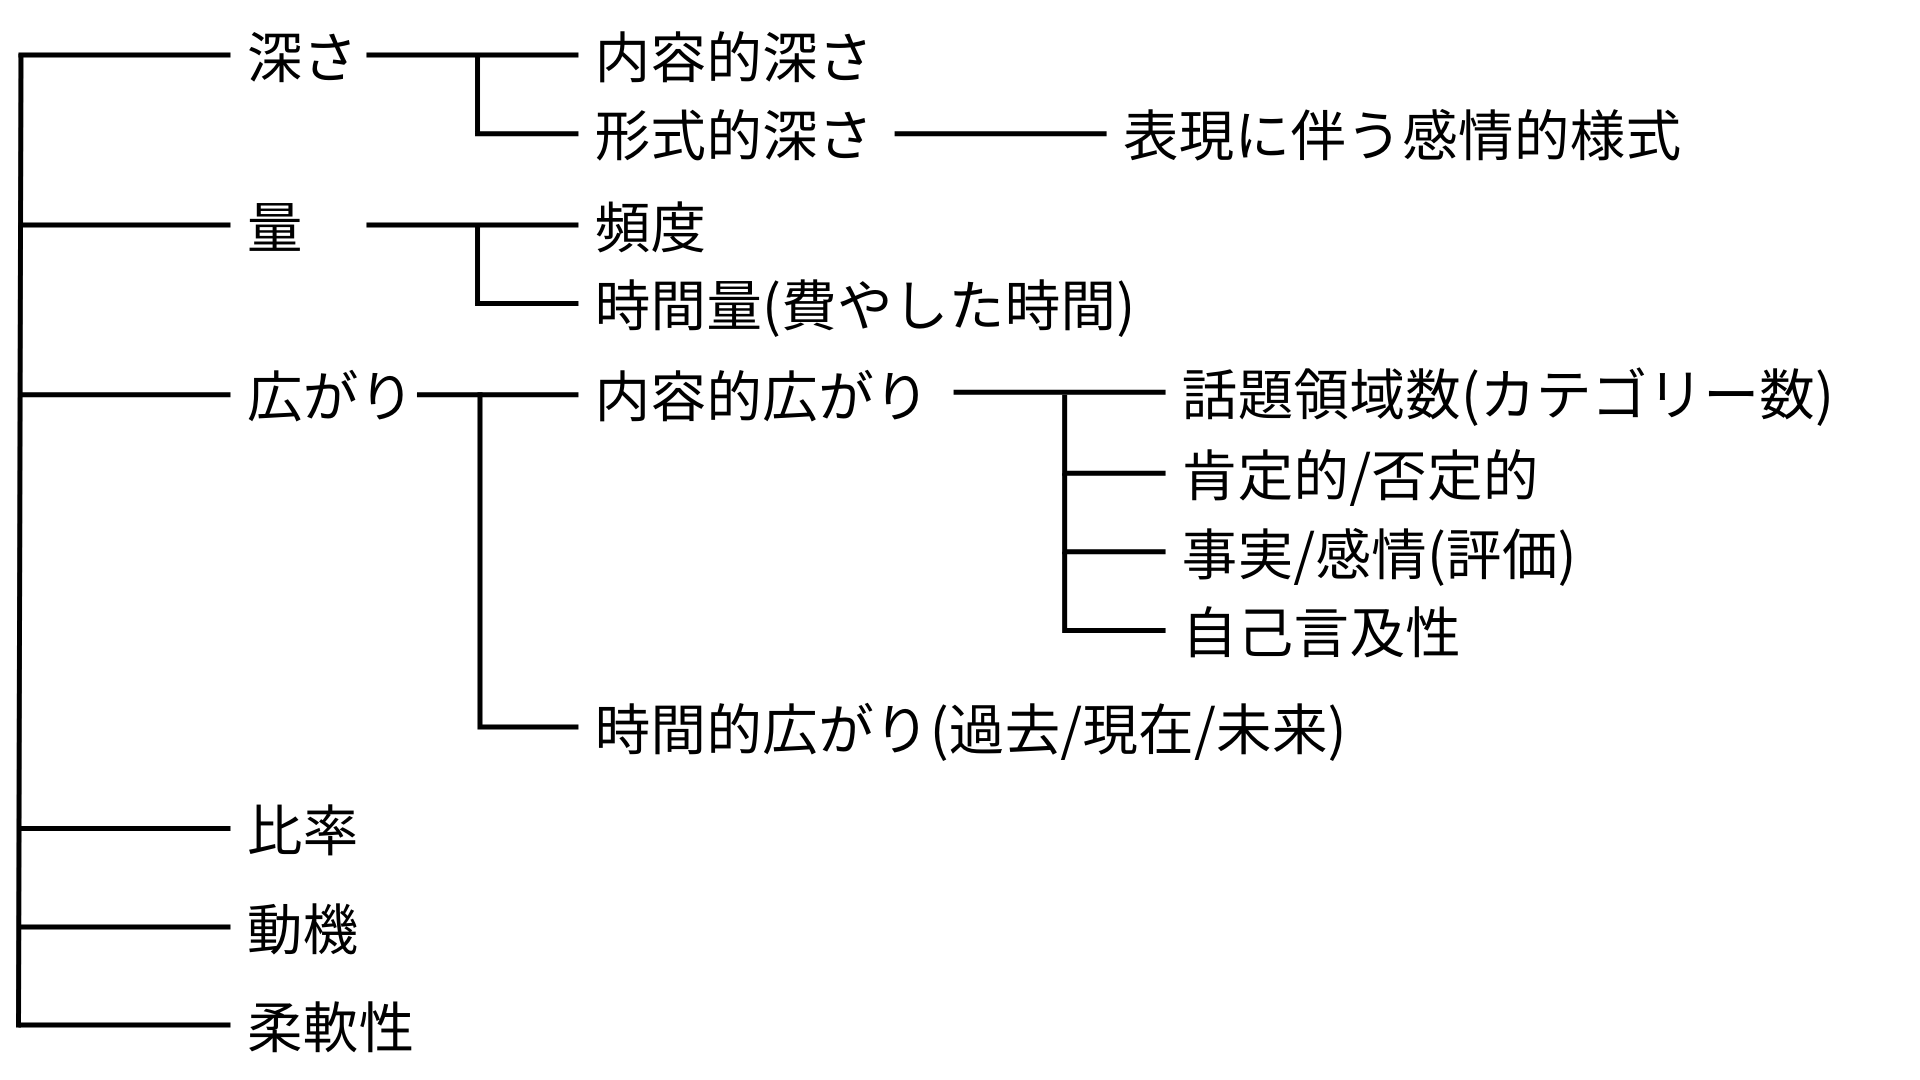
\includegraphics[width=0.75\linewidth]{image/自己開示の次元.png}
    \caption{自己開示の次元}
    \label{fig:自己開示の次元}
\end{figure}

% ＜各次元の説明（全て榎本を参考に）＞
深さの次元は，内容的深さと形式的深さに分類される．内容的深さは開示される情報の本質的な深さを表し，表層的な事実から内面的な感情まで段階的に変化する．形式的深さは表現に伴う感情的様式を示し，感情表現の強さや直接性の程度を反映する．榎本は，この深さの次元が親密な関係性の発展において特に重要な役割を果たすことを指摘している．
量の次元は，自己開示の頻度と費やした時間量で測定される．
広がりの次元は，内容的広がりと時間的広がりから構成される．内容的広がりには話題領域数，肯定性/否定性，事実/感情，自己言及性といった次元が含まれ，自己開示の多様性を表す．時間的広がりは過去・現在・未来にわたる開示の範囲を示し，時間軸における開示内容の分布を反映する．
比率の次元は全体的なコミュニケーションにおける自己開示の割合を表し，関係性の質を反映する指標となる．
動機の次元は，自己開示を行う理由や目的を示し，関係性の発展や維持における意図的な側面を反映する．
柔軟性の次元は状況や相手に応じて自己開示の程度を調整する能力を表し，社会的スキルの一側面として捉えられる．

% その中で，深さに着目する理由を述べる．
Collinsら\cite{collins_1994}のメタ分析によると．自己開示の量よりも深さが好意形成に大きな効果をもたらすことが示されている．また社会的浸透理論という理論では．関係性は自己開示の深さと広さの段階的な増加を通して発展することが提案されている．これらの知見に基づき，本研究では，親密化の過程における影響が大きいとされる深さに着目する．次項では，この自己開示の深さについて社会的浸透理論を元に詳しく論じる．



\subsection{自己開示の深さ}\label{自己開示の深さ}

自己開示における深さとは，開示される個人的な情報の度合いを指す．Derlega\cite{derlega_1993_self_disclosure}によれば，表面的な事実（趣味や職業など）から，内面的な感情（家族の問題や人生の目標に関する感情など）まで，様々な深さの段階が存在する．

自己開示の深さについて，Altman・Taylor（1973）の見解を榎本は以下のように整理している：
\begin{enumerate}
    \item 特定の状況下の個々の行動の開示より，性格特性のようなより普遍的な傾向の開示のほうが深い
    \item 独自な内容の開示ほど深い
    \item 行動や実際の出来事よりも，動機・感情・空想のような目に見えない側面の開示ほど深い
    \item 自分の弱点にふれる内容の開示ほど深い
    \item 社会的に望ましくない側面の開示ほど深い
    \item 強い感情を伴う開示ほど深い
\end{enumerate}

このような深さの概念を体系的に説明する理論として，社会的浸透理論（Social Penetration Theory）がある．

\subsection*{社会的浸透理論}
社会的浸透理論では，2者間の相互作用が表面的なレベルから親密なレベルへと進展し，人間関係が親密化していく過程を社会的浸透（Social Penetration）という概念で説明している．この理論では，人間関係における自己開示の深まりを玉ねぎの層に喩え，表面的な層から徐々により深い層へと進展していく段階的なプロセスをモデル化している．図\ref{fig:onion-model}に自己開示の段階を表す玉ねぎモデルを示す．

\begin{figure}[H]
    \centering
    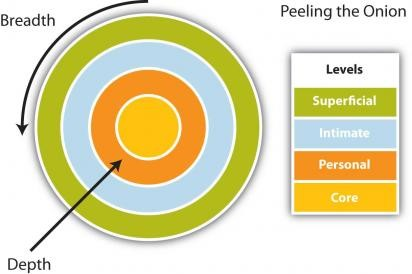
\includegraphics[width=0.75\linewidth]{image/onion-model.png}
    \caption{自己開示の段階を表す玉ねぎモデル}
    \label{fig:onion-model}
\end{figure}

Poseyら\cite{posey_2010}は内側の親密な層が明らかにされる前に，外層の部分が順番に露出し，経験され，剥がされなければならないと述べており，自己開示の深まりには段階的なプロセスが必要であることを指摘している．

また，社会的浸透理論において，自己開示の各層は以下のように整理されている．

\begin{enumerate}
    \item 表層：服装や音楽の好き嫌いなど，比較的浅い情報
    \item 中間層：政治的な見解，社会的な態度
    \item 内層：精神的な価値観，深い恐れ，希望，目標，空想，秘密
    \item 核：その人に関する最もプライベートな情報
\end{enumerate}

本項では，社会的浸透理論に基づき自己開示の深さについて論じた．自己開示は表層的な内容から徐々により深い内容へと段階的に進展していくプロセスを経ることを示し，玉ねぎモデルで4つの層に分けて整理した．自己開示の深さには，様々な状況要因が影響を与えることが知られている．次項では，自己開示の促進に関わる状況要因について説明する．



\subsection{自己開示に影響する状況要因}\label{状況要因}

自己開示は状況とも密接な関係がある．榎本は，自己開示に影響を与える状況要因として，相手の性別，人種，魅力度（外見など），両者の地位関係，部屋のつくりや装飾，視線，自意識の喚起度，生理的条件（飲酒等）など，多くの要因を指摘している．しかし，最大の要因は相手の自己開示の程度，すなわち自己開示の相互性であると述べており，この要因は個人差を打ち消してしまうほど強い影響力を持つことが，多くの研究により実証されている．


\subsection*{自己開示の相互性}\label{自己開示の相互性}

榎本は自己開示の相互性とは，相手の開示レベルに合わせて自分も開示しようとする傾向であると述べる．相手が浅い自己開示しかしない場合，こちらも浅い自己開示しか行わず，相手が深い自己開示をした場合には，こちらも深い自己開示をするというものである．深田\cite{深田_2000}は，自己開示は開示相手にとって報酬的な意味を持ち，お返しの自己開示を促進することにより，自己開示の相互性が次第に高まり，その結果2者関係が発展すると述べている．
榎本は，自己開示の相互性の時系列的変化についても言及している．表層的な自己開示の相互性については，関係の初期に最も頻繁に表れ，次第に減少していく．一方，深い自己開示の相互性は，関係の初期にはほとんど見られないがしだいに増してゆき，中盤でピークを迎えやがて減少していくという．

% 相互性の崩壊（対象でない関係段階）について
% ただし，この相互性は必ずしも成り立つわけではない．榎本によれば，初対面の関係や非常に親密な関係では，この相互性は崩壊する傾向にあるという．初対面の状況では，自己開示が一定のレベルを超えると，お互いの現在の関係から予期される水準を大きく上回り，開示者に対する不信感が生じる．一方，非常に親密な関係では，既に強固な信頼関係が成立しているため，必ずしも自己開示の返報を必要しないという．

% 総論
上記の通り自己開示の相互性の研究より，相手が自己開示をした際に，最も抵抗なく自己開示をすることができるということが示唆された．自己開示は単一方向的なものではなく，開示者と被開示者の間での相互作用だと考えられる．具体的には，Aの自己開示に対してBが受容をし，その後Bが同程度の自己開示を行うという循環的なプロセスが存在する．このプロセスにおいて，被開示者の受容が重要な役割を果たすことから，次節では自己開示の受容について詳しく検討する．
\section{自己開示の受容}\label{受容}

前節で述べたように，自己開示が開示者と被開示者の間での相互作用であり，特に自己開示の相互性のプロセスにおいて被開示者の受容が重要な役割を果たすと述べた．そこで本節では，自己開示の受容に焦点を当て，自己開示の促進と，人間関係の発展に果たす役割と影響について説明する．

% --------------------------------------------------------------------------------------------------------

\subsection{受容の定義}

被開示者の反応は，受容と拒絶の2つに分けられる．森脇\cite{森脇_2005}によると，被開示者の受容には「聴く際の真摯な姿勢」「アドバイス」「親身な行動」「共感」，拒絶には「否定・無視」「無関心」「聴く際の真剣味のなさ」「無反応」といった多様な反応が含まれる．これらを踏まえ，川西は，相手の自己開示に対する受容を「開示者に対する肯定的・共感的反応」，拒絶を「開示者に対する否定的・非共感的反応」と定義している．


\subsection{自己開示の促進に与える影響}\label{}

受容は自己開示の促進に重要な役割を果たすことが示されている．相川\cite{相川充_2010}によれば，相手の共感的な反応を通じて受容されていると感じることで，開示者はより内面的な自己開示へと動機づけられるという．この過程について，Weber\cite{weber_2004}の研究では2つの重要な知見が示されている．第一に，親密な相手から思いやりや共感を受けることで，相手に理解されているという感覚が高まることと，第二に，親密な相手からの思いやりや共感を受けることは，相手に対して意図的に自己開示を行おうとする傾向と関連があることが示されている．
% ただし，実際の自己開示の量や深さとの関連は見られなかったことから，思いやりや共感の表現は，自己開示の行動そのものよりも，開示しようとする意図に影響を与える可能性が示唆されている．

対照的に，自己開示に対する拒絶的な反応は，開示者に心理的な傷つきをもたらし，その後の自己開示を抑制する可能性がある．拒絶的な反応を経験した個人は，その後の人間関係において防衛的になり，深い自己開示を避ける傾向があることが指摘されている．

このように，被開示者から受容されたという感覚は，さらなる自己開示を促進すると考えられる．また，受容的反応は自己開示の促進だけでなく，関係の親密化においても重要な役割を果たすことが明らかになっている．次項では，受容が関係の親密化に与える影響について説明する．



\subsection{関係の親密化に与える影響}\label{}

前項で述べたように，受容は自己開示を促進するだけでなく，関係の親密化においても重要な役割を果たすことが明らかになっている．榎本は，自己開示に対する受容が開示者の自尊心を高め，2者間の人間関係が親密化することを指摘している．

この関係性について，Reis\cite{reis_2017}は理解（understanding）という概念から詳細な説明を行っている．理解とは相手の経験や特性についての知識や認識を持つことであり，理解されていると感じることは関係性の質を高めることが示されている．さらに，Weberの研究によれば，思いやりや共感の表現は，お互いの信頼関係を深める要因となることが示されている．

相手からの思いやりや共感を受けることで相手に理解されているという感覚が高まり，それが結果として関係性の質の向上につながると考えられる．これらの知見は，自己開示に対する受容的な反応が，単に自己開示を促進するだけでなく，関係の親密化に重要な役割を果たしていることを示している．


\subsection{自己開示に対する受容の課題}\label{受容の課題}
% ここまでは受容の重要性を述べた → その難しさ → それを解決する必要あり(?)
これまで述べてきたように，自己開示の受容は人間関係の親密化において重要な役割を果たす．しかし，自己開示に対する適切な受容は必ずしも容易ではない．特に深い自己開示を受けた際，被開示者は適切な反応を示すことに困難を感じることがある．
表層的な自己開示に対しては比較的容易に受容できるが，深い自己開示に対しては，より慎重で共感的な反応が必要となる．

% 受容側に着目した研究少ない．やる必要あるって話
川西が，従来の研究では被開示者の受容が前提とされる場合の効果に関するものがほとんどであると指摘しているように，既存研究では，開示者側に着目した研究が多く，被開示者の受容に着目したものは比較的少ない．しかし，自己開示した際，相手に必ずしも受け入れられるとは限らない．特に，深い自己開示は過去のトラウマや失敗など，否定的側面を含むことが多い．開示内容が否定的である場合，批判や誤解を招く可能性や無関心な態度を取られる可能性が十分にある．

\section{音楽嗜好を通じた自己開示}\label{音楽}
前節までで述べたように，自己開示は人間関係の親密化に重要な役割を果たすものの，現代の若者は深い自己開示を避ける傾向にある．また，深い自己開示に対しては，より慎重で共感的な反応が必要となる．この課題に対して，本研究では音楽嗜好を通じた自己開示に着目する．音楽嗜好は以下に挙げる4つの特徴を持つことから，自己開示を深めていく場合に適していると考えられる．


\subsubsection{パーソナリティとの関係}
Rentfrowら\cite{rentfrow_2003}\cite{rentfrow_2006}\cite{rentfrow_2007}の研究により，音楽嗜好とパーソナリティの間に有意な相関があることを実証的に示されている．具体的には，個人の音楽嗜好が，その人の性格特性，価値観，および認知的特徴を反映する傾向があることが明らかにされている．
このような音楽嗜好とパーソナリティの密接な関係性は，音楽を通じた自己開示が単なる趣味の共有以上の意味を持つことを示唆している．すなわち，音楽嗜好について語ることは，個人の内面的な特性を自然な形で表現する手段となる．


\subsubsection{普遍性}
音楽の普遍性は，対人コミュニケーションにおいて重要な意味を持つ．音楽は多くの人々が日常的に接している文化的要素であり，たとえ特定のアーティストや楽曲に対する知識の差があったとしても，共通の話題として取り上げやすいためである．つまり，音楽嗜好は会話のきっかけとして機能しやすく，自己開示を自然に促進する要素となる．


\subsubsection{楽曲に紐づく経験や感情}
音楽は，個人の経験や感情と密接に結びつく特性を持っている．この特性は，自己開示のプロセスにおいて重要な役割を果たす．具体的には，音楽に関する自己開示は，ジャンルや曲名といった表層的な情報の共有から始まり，特定の楽曲に対する個人的な思い入れや経験の共有へと，段階的に深化させることが可能である．例えば，特定の楽曲は，恋愛経験や人生の転機といった重要な個人的経験と結びついていることが多い．また，精神的な困難に直面した際の心理的支えとして機能することもある．


\subsubsection{音楽活動による絆の形成}
音楽活動による社会的な結びつきの形成について，Tarrら\cite{tarr_2014}は，社会的動機づけや快感，報酬に関わる神経系である内因性オピオイド系（EOS）と自己-他者の融合という2つのメカニズムに着目している．音楽の受動的な聴取でもEOSが活性化され，社会的な結びつきの形成が促進されることを示唆している．具体的には．音楽聴取がストレス軽減や気分の改善などの効果をもたらし，これらが人々の結びつきを促進する基盤として機能することが指摘されている．

\vskip\baselineskip

% 音楽嗜好を通じた自己開示がいいんすよ の話
これらの特徴から，現代の若者は音楽嗜好の共有をきっかけとして，その音楽にまつわる経験や個人的な価値観を話すことで，自然な流れで自己開示を行うことができる．このような段階的な相互開示のプロセスは，より深い相互理解と親密な関係性の構築へとつながると期待される．
\section{研究目的}

% ＜改めて背景を洗う + 若い世代である必要性＞
ここまでに述べたように，自己開示は人間関係の親密化において重要な役割を果たす．特に，段階的な自己開示のプロセスとそれに対する適切な受容は，関係性の親密化に不可欠な要素である．しかし，現代では否定や拒絶への不安から深い自己開示を避ける傾向にあり，人間関係の希薄化につながっている．
% ＜音楽という新しいアプローチ＞
この課題に対し，1.4節で述べたように，音楽嗜好の共有は有効なアプローチとなる可能性がある．音楽は個人の価値観や感情を反映する要素であり，その共有をきっかけとして音楽にまつわる経験や個人的な価値観を語り合うことで，自然な形での自己開示が期待できる．

% ＜目的＞
以上より，本研究では，音楽嗜好の共有を通じた自己開示を促進することで，関係の親密化を目指す．

% 2章
\chapter{音楽嗜好の共有による自己開示}\label{世界観}
前章では，自己開示が人間関係の親密化において重要な役割を果たすことを述べ，特に社会的浸透理論に基づく段階的な自己開示の重要性を指摘した．その上で，音楽嗜好の共有を通じた自己開示が，若者の人間関係の親密化を促進する可能性があることを示した．

本章では，音楽嗜好の共有を通じた自己開示を行う具体的な環境について述べ，社会的浸透理論に基づいた段階的な自己開示を促進するための要件を提案する．


\section{音楽嗜好の共有が適している環境}\label{音楽嗜好の共有が適している環境}
% 〇〇ではこういうのが問題で～
音楽嗜好の共有を通じた自己開示には，音楽ストリーミングサービスでのプレイリストの共有，SNSでの音楽体験の発信，あるいは日常会話での好みの表明など，様々な形態が存在する．しかし，これらの方法では好みの表明が一方向的になりやすく，相互の深い理解や受容を促進する機会として十分に機能しない．

% こういう条件が必要で～
榎本が指摘するように，自己開示は状況と密接な関係があり，環境要因が大きく影響する．深田は，特に相手からの受容が自己開示を促進する重要な要因であることを示している．これらの知見に基づけば，効果的な自己開示の実現には，自己開示の相互性と受容を考慮した適切な環境が必要となる．そのため，音楽嗜好の共有を通じた自己開示には以下に挙げる3つの条件を満たす環境が望ましい．


\subsubsection{音楽の実体験の共有}
音楽嗜好の共有を通じた自己開示の場においては，単なる好みの表明だけでなく，実際の音楽を共に聴く，歌うといった形で体験できることが重要である．Tarrの研究によれば，音楽の共同体験は社会的絆の形成を促進し，他者との心理的な結びつきを強める効果がある．また，榎本が指摘するように，自己開示は言語的なものに限らず，非言語的な表現も含む多様な形態を持つ．音楽体験を共有することは，感情や印象をリアルタイムで共有することを可能にし，自己開示と自己開示に対する受容を促すことができる．


\subsubsection{明示的な相互性の確保}
\ref{状況要因}項でも述べたように，自己開示の状況要因で最も影響の強いとされるのは自己開示の相互性である．そのため，片方の一方的な開示に偏ってしまわないよう，音楽を聴く側と開示（表現）する側の役割が明確に分かれ，それらを交互に行う構造が必要である．


\subsubsection{対面での交流}
Weberの研究によれば，思いやりや共感の表現は相手に理解されているという感覚を高め，信頼関係を深める．対面での交流は，相手の反応や表情から受容を直接的に確認することを可能にし，それが次の自己開示を促進する重要な要因となる．また，Reisが指摘するように，対面でのコミュニケーションは相互理解の深化において重要な役割を果たす．

\vskip\baselineskip

% それを満たすのはカラオケで～
以上の条件を総合的に満たす環境として，本研究ではカラオケに着目する．カラオケは，音楽を通じた自己開示や自己表現が自然に行われる場\cite{烏賀陽弘道_2005}であるように，選曲や歌唱を通じた音楽の実体験を共有できる場と言える．さらに「歌う」「聴く」という明確な「開示者」と「被開示者」としての役割が存在することにより相互作用が生まれやすい．これらの特徴は，前述した条件を効果的に満たしており，音楽の共有を通じた自己開示をする環境として適しているといえる．
\section{自己開示の場としてのカラオケ}\label{自己開示の場としてのカラオケ}
カラオケは，音楽を介した相互作用が生まれる社会的な場である．本節では，カラオケにおける自己開示と受容の定義を明確にし，その特徴について論じる．

\subsection{カラオケにおける自己開示と受容}
\subsection*{カラオケにおける自己開示の定義}

自己開示とは，\ref{自己開示の定義}節でも述べたように，言語的なコミュニケーションに限らず，非言語的な表現も一形態である．また，受容についても非言語的・言語的の両面から評価可能な形で定義づける必要がある．

単に曲名を相手に伝えるだけでは，自己開示にならない．そこで，曲を実際に流し，歌唱をする，またそれに伴いなぜそれが好きであるか，なぜそれを選曲したかといった動機を相手に伝える行為こそが，カラオケにおける自己開示になると考える．

そこで，本研究における自己開示とは，音楽選択による自己表現と，その選択に関する言語的説明の2つの要素とする．音楽選択による自己表現とは，個人の好みや価値観が反映された楽曲を選択し他者と共有する行為を指す．選択に関する言語的説明とは，選曲理由や楽曲にまつわる個人的経験，感情などの言語的な共有を指す．


\subsection*{カラオケにおける受容の定義}
本研究における受容とは，①相手の選択した音楽を傾聴する非言語的受容と，②音楽や説明に対する共感や理解を示す言語的受容の2つの要素から構成される．これらの要素は，相手の自己開示に対する肯定的な反応として機能する．


\subsection{カラオケにおける自己開示の特徴}

カラオケにおける自己開示の特徴として，実体験を伴う開示が挙げられる．通常の会話では音楽の好みを口頭で開示することに留まり，曲名や好みの表明のみでは相手に音楽の本質的な魅力を伝えることは難しい．一方でカラオケでは，実際の楽曲が流れ，その曲調やメロディー，リズムといった音楽的特徴を直接体験として共有できる．さらに，歌唱を通じて自身がその楽曲のどの要素に魅力を感じているのかを，より具体的かつ直接的に表現することが可能となる．
また，カラオケにおける自己開示は，好みの曲の共有から感情の開示まで，段階的な開示が存在すると考えられる．好みのアーティストの楽曲を選択することから始まり，その選曲理由や曲への思い入れが語られ，さらに歌唱を重ねる中で思い出や個人的な感情が共有される．このように，カラオケは音楽の選曲と歌唱を通じて，徐々に内面を開示していくためのきっかけとして機能すると考えられる．

さらに重要な特徴として，明確な役割分担による相互性の確保がある．数家\cite{数家鉄治_2008}が指摘するように，カラオケは共同行為に必要な自己と他者の相互依存性をより緊密にできる場である．「歌を歌う」「相手の歌を聴く」という明確な役割が交互に繰り返される構造は，自己開示の相互性を自然な形で実現する．これにより通常の会話場面では，実現が困難である明示的な相互の自己開示や，自己開示のバランスの制限をすることが可能となる．

\vskip\baselineskip

これらの特徴から，カラオケが音楽嗜好の共有を通じた自己開示の環境・状況として有効であると考える．
\section{カラオケにおける自己開示の深さ}\label{カラオケにおける自己開示の深さ}
本節では，カラオケにおける自己開示の深さについて整理する． 

\subsection{既存の自己開示尺度}
これまでに開発された自己開示を測定できる尺度としては，榎本の「自己開示質問紙」\cite{榎本_1997_自己開示の心理学的研究}や，丹羽・丸野の「自己開示の深さを測定する尺度」\cite{自己開示尺度}が挙げられる．しかし，これらの心理尺度は，自己開示の項目や話題内容ごとに深さが定義されているのみで，音楽嗜好の共有について自己開示の深さを定義しているものではない．また，従来の研究では「音楽の好み」を1つの自己開示の項目として扱うのみで，その内部構造や深さについては既存研究では行われていない．

カラオケにおける自己開示は，曲に対する思い入れの深さ，その曲を開示するときに相手が知っているかどうかといった認知度，上手に歌えるかといった不安感などの様々な要素が影響し，一元的な尺度として示せるものではない．次項ではその構成要素について整理する．



\subsection{自己開示を構成する3軸}\label{3軸}
カラオケにおける音楽嗜好の共有を通じた自己開示を，\ref{自己開示の深さ}項で述べた榎本の整理した自己開示の深さと，伊藤\cite{カラオケにおける自動楽曲推薦}による「あなたはカラオケで選曲をする際，どんなことを考慮して選びますか？」というアンケート調査の結果より，以下の3つの軸で整理を行った．

\subsection*{1. 思い入れ}
思い入れは楽曲に対する個人的な愛着や経験の深さを表す主観的指標である．榎本が指摘するように，内面的な感情や動機の開示は自己開示の深さを特徴づける重要な要素である．思い入れの強い楽曲の選択は，その人固有の価値観や感情の表出を伴うため，より深い自己開示となる．

\subsection*{2. 歌うことの自信}
歌うことの自信は楽曲を歌唱する際の技術的な自信度を表す主観的指標である．アンケート調査において「歌いやすい，または自分の得意な曲」は，重要な選曲基準として挙げられたように，音域やリズムの難易度に対する自己評価の高いものが選ばれやすい．特に自身の歌唱能力における弱点の開示は，榎本の指摘する「弱点や欠点の開示」という深い自己開示の要素と合致する．

\subsection*{3. 人気度}
人気は楽曲の社会的認知度を表す客観的指標である．アンケート調査において「みんなが知っているかどうか」が選曲基準であるように，楽曲の認知の度合いは自己開示のしやすさを決めるうえで重要な要素である．例えば，非常にマイナーな曲を開示することは，相手に否定されるかもしれない，知らなかったら楽しめないかもしれないという否定的側面を伴うため，自己開示の深さを示す指標としてふさわしいと考えられる．

なお，テンポや歌詞の特徴といった要素は，個人の好みの差が大きく一律の指標として扱うことが困難であるため，本研究では除外する．


\subsection{自己開示を促す手法} % 段階的に自己開示するのがええんやで

% ① 玉ねぎの内側にたどり着くためには，外側から攻める必要がある
社会的浸透理論をレビューしているCarpenter\cite{carpenter_2015_SPT_Review}は，「玉ねぎモデルは，人々が対人的な相互作用を通じて他者の個人的情報の層を剥がしていき，核心に到達するというプロセスとして社会的浸透を説明する有用な比喩」と述べている．すなわち，個人の内面に関する思い入れや経験を引き出すには，その外側である一般的な音楽の好みを共有することから始める必要がある．
% ②いきなり深い自己開示をしても受容できない
\ref{受容の課題}項で述べたように，深い自己開示をいきなり行った場合，相手はそれを十分に受容することができない．カラオケにおいても，思い入れの強い曲や知名度の低い曲をいきなり選曲することは，相手の受容を得られにくい．そのため，多くの人は相手が知っている曲を選曲するなど，表面的な好みの共有に留まってしまう傾向がある．

そのため，カラオケにおける音楽嗜好の共有を通じた自己開示は，好きなアーティストや，普段歌う曲といった一般的な嗜好の共有から始まり，特定の楽曲への思い入れ，そして人生において重要な意味を持つ楽曲の共有へと，徐々に深めていくことが重要であると考えられる．このように音楽を介することで，自然な形での深い自己開示が可能となる．

しかし，このような段階的な自己開示を行う場合には，何らかの方法で自己開示を促す必要がある．次節では，カラオケ環境において段階的な自己開示を促進するための方法について検討する．
\section{関連研究}\label{関連研究}
\begin{comment}
・自己開示をシステムが促すことで親密度が向上するんだよーっていうKDDIの研究をかく
・カラオケでの楽曲推薦とかも必要そうなら挙げる
・カラオケにはシステムがあるから，介入させるのが自然だよね（既存のDAMやJOYSOUNDでrecommendされてることを記す）

→ システムを使うことが有効そう だと示唆する
\end{comment}

\subsection{自己開示の促進支援に関する研究}
池田ら\cite{自己開示の促しによるコミュニケーション支援システム}の研究は，自己開示を促進するコミュニケーション支援システムの有効性を示した重要な知見を提供している．池田らは婚活パーティーを想定し，初対面の2人の参加者間でタブレット端末に話題を表示するシステムを開発した．話題には「趣味」や「休日の過ごし方」といった自己開示項目を用い，(1)自己開示の深さを考慮して段階的に話題を提示する手法，(2)ランダムに話題を提示する手法，(3)システムを用いない条件の3つの方法で12分間の会話実験を行った．192名の参加者による大規模な実験の結果，システムによる自己開示の促進が，参加者間の親密度向上に有意な効果をもたらすことを実証した．また，段階的な提示手法では，提示された話題への興味や言及のしやすさ，システムの継続利用意向といった評価指標において，ランダム提示手法より高い評価を得ることが確認された．ただし，システムへの過度な依存や自然なコミュニケーションの阻害といった課題も指摘されており，ユーザの自由度を保ちながら必要な時にのみ支援を提供することの重要性が示唆されている．

\subsection{カラオケ環境における支援システム}
カラオケ環境は，システムによる介入が自然に受け入れられる特徴を持つ．選曲の際にタブレット端末を使用することが一般的であり，システムからの情報提示に対する抵抗感が低いと考えられる．実際に，田中ら\cite{tanaka_2020}によって開発されたレコメンドシステムがDAM\cite{DAM}のカラオケシステム「LIVE DAM Ai」に導入されているように，楽曲推薦による支援が実用化されている．このような特性は，自己開示を支援するシステムを導入する上で大きな利点となり得る．

\vskip.5\baselineskip

本研究では，これらの知見を踏まえ，カラオケ環境の特性を活かしながら，自然なコミュニケーションを阻害しない形での自己開示支援システムの設計を目指す．
\section{研究課題と仮説}\label{研究課題と仮説}

先行研究から，本研究では音楽嗜好の共有を通じた自己開示の場としてカラオケ環境を利用する．特に，自己開示の深さを考慮して，段階的に自己開示を促すシステムの導入により，コミュニケーションを阻害することなく効果的な自己開示が促進される可能性がある．この知見に基づき，以下の研究課題と，その課題を明らかにするための仮説を設定する．

\subsubsection{課題:カラオケ空間における音楽嗜好の段階的な自己開示が受容性に及ぼす影響}

WeberやReisらの研究では，相手の経験や感情を理解し受け入れる受容性が，良好な対人関係の構築に不可欠であることが示唆されているが，音楽嗜好の共有を通じた自己開示が受容に与える影響については十分な検討がされていない．そこで本研究では，カラオケ空間における段階的な自己開示が他者受容性に及ぼす影響を実証的に検証する．

\subsubsection{仮説1:低いレベルから高いレベルへと段階的に自己開示を行うことで，深いレベルの自己開示に対する受容度が高くなる}

仮説1は，社会的浸透理論に基づいており，対人関係の発展過程において自己開示が段階的に深まることを前提としている．突発的な深い自己開示は相手が受容できない可能性があるが，浅い自己開示から始めることにより，被開示者は開示者の個人的な経験や感情をより自然に受容できると考えられる．

\subsubsection{仮説2:音楽への認知度が低い，または興味度が低い場合でも，自己開示の受容度は大きく低下しない}

音楽嗜好の共有を通じた自己開示において，被開示者が必ずしも同じ楽曲への認知や興味を持っているとは限らない．しかし，段階的な自己開示手法を用いることで，音楽そのものへの興味の有無に関わらず，開示者の経験や感情を理解し受容できると考えられる．

\subsubsection{仮説3:セッションを終えた2者は，段階的に自己開示を促していない方に比べて相手に対する受容性が向上する}

適切な段階を経た自己開示は，開示者と被開示者の双方に安心感をもたらし，相手の経験や感情に対する理解と受容を深める．これにより，セッション後の2者間における相互の受容性が，段階的な支援がない場合と比較して向上すると考えられる．

\vskip\baselineskip

これらの仮説を検証するためには，段階的な手法の効果を明確に評価できる環境から始めることが重要である．カラオケ環境では，歌唱による本人の緊張感や，歌唱の技術レベルといった個人特性が大きく影響する．また，歌唱そのものの楽しさや，共同で場を作り上げることによる自然な親密度の向上など，多くの要因が複雑に絡み合っている．これらの要因は自己開示の促進効果を正確に測定することを困難にする可能性がある．そこで本研究ではまず，カラオケの環境に近しい状態で歌唱という要素を除いた「音楽共有セッション」を行うこととする．音楽共有セッションにおいて自己開示を段階的に促進する楽曲推薦システムと，段階的な促進を行わないシステムを用いた比較実験を行う．これにより，音楽を介したコミュニケーションにおける自己開示と受容性の基礎的な知見を明らかにした上で，将来的に歌唱を伴うカラオケ環境特有の要因を考慮した検証へと発展させることを目指す．
% 3章
\chapter{評価実験}
本章では，段階的に自己開示を促すことによる受容性の変化を検証するため，評価実験を行う．実験に用いる自己開示を促す楽曲推薦システムの設計・実装について述べ，実際に楽曲推薦システムを使用し，どのように評価を行うかについて述べる．

% 本章では，カラオケにおける自己開示のモデルを3軸で整理する．そして，この3軸に基づいた自己開示レベルの定義と分類方法について述べる．最後に，これらのモデルを実装した実験支援システムの詳細について説明する．

% -----------------------------------------------------------------------------------------
\section{実験設計}

本節では，実験目的，実験条件，実験手順について述べる．

\subsection{実験目的}
本実験は，段階的な自己開示支援が受容性の向上に与える効果を検証することを目的とする．提案手法が自己開示の深化と受容性の向上に寄与するかを明らかにするため，システムによる段階的支援の有無による比較実験を実施する．


\subsection{実験条件}

\subsubsection{実験環境}

実験はカラオケ空間をもした閉鎖的な空間で実施した．対面でのカジュアルな会話を促進するため，2つの座椅子を適度な距離を保って対面に配置し，Bluetoothスピーカーを通じて音楽を再生する．カラオケ店舗の雰囲気を模倣するため，YouTube\cite{youtube}で配信されているDAMチャンネル\cite{damchannel}の動画コンテンツを小音量で再生し，完全な無音空間を避けるようにした．また，実験室の壁面にプロジェクターでDAMチャンネルの映像を投影し，視覚的な要素も考慮した．照明は会話に支障をきたさない程度の明るさに調整することで，リラックスした雰囲気の実現を図った．

\begin{figure}[H]
    \centering
    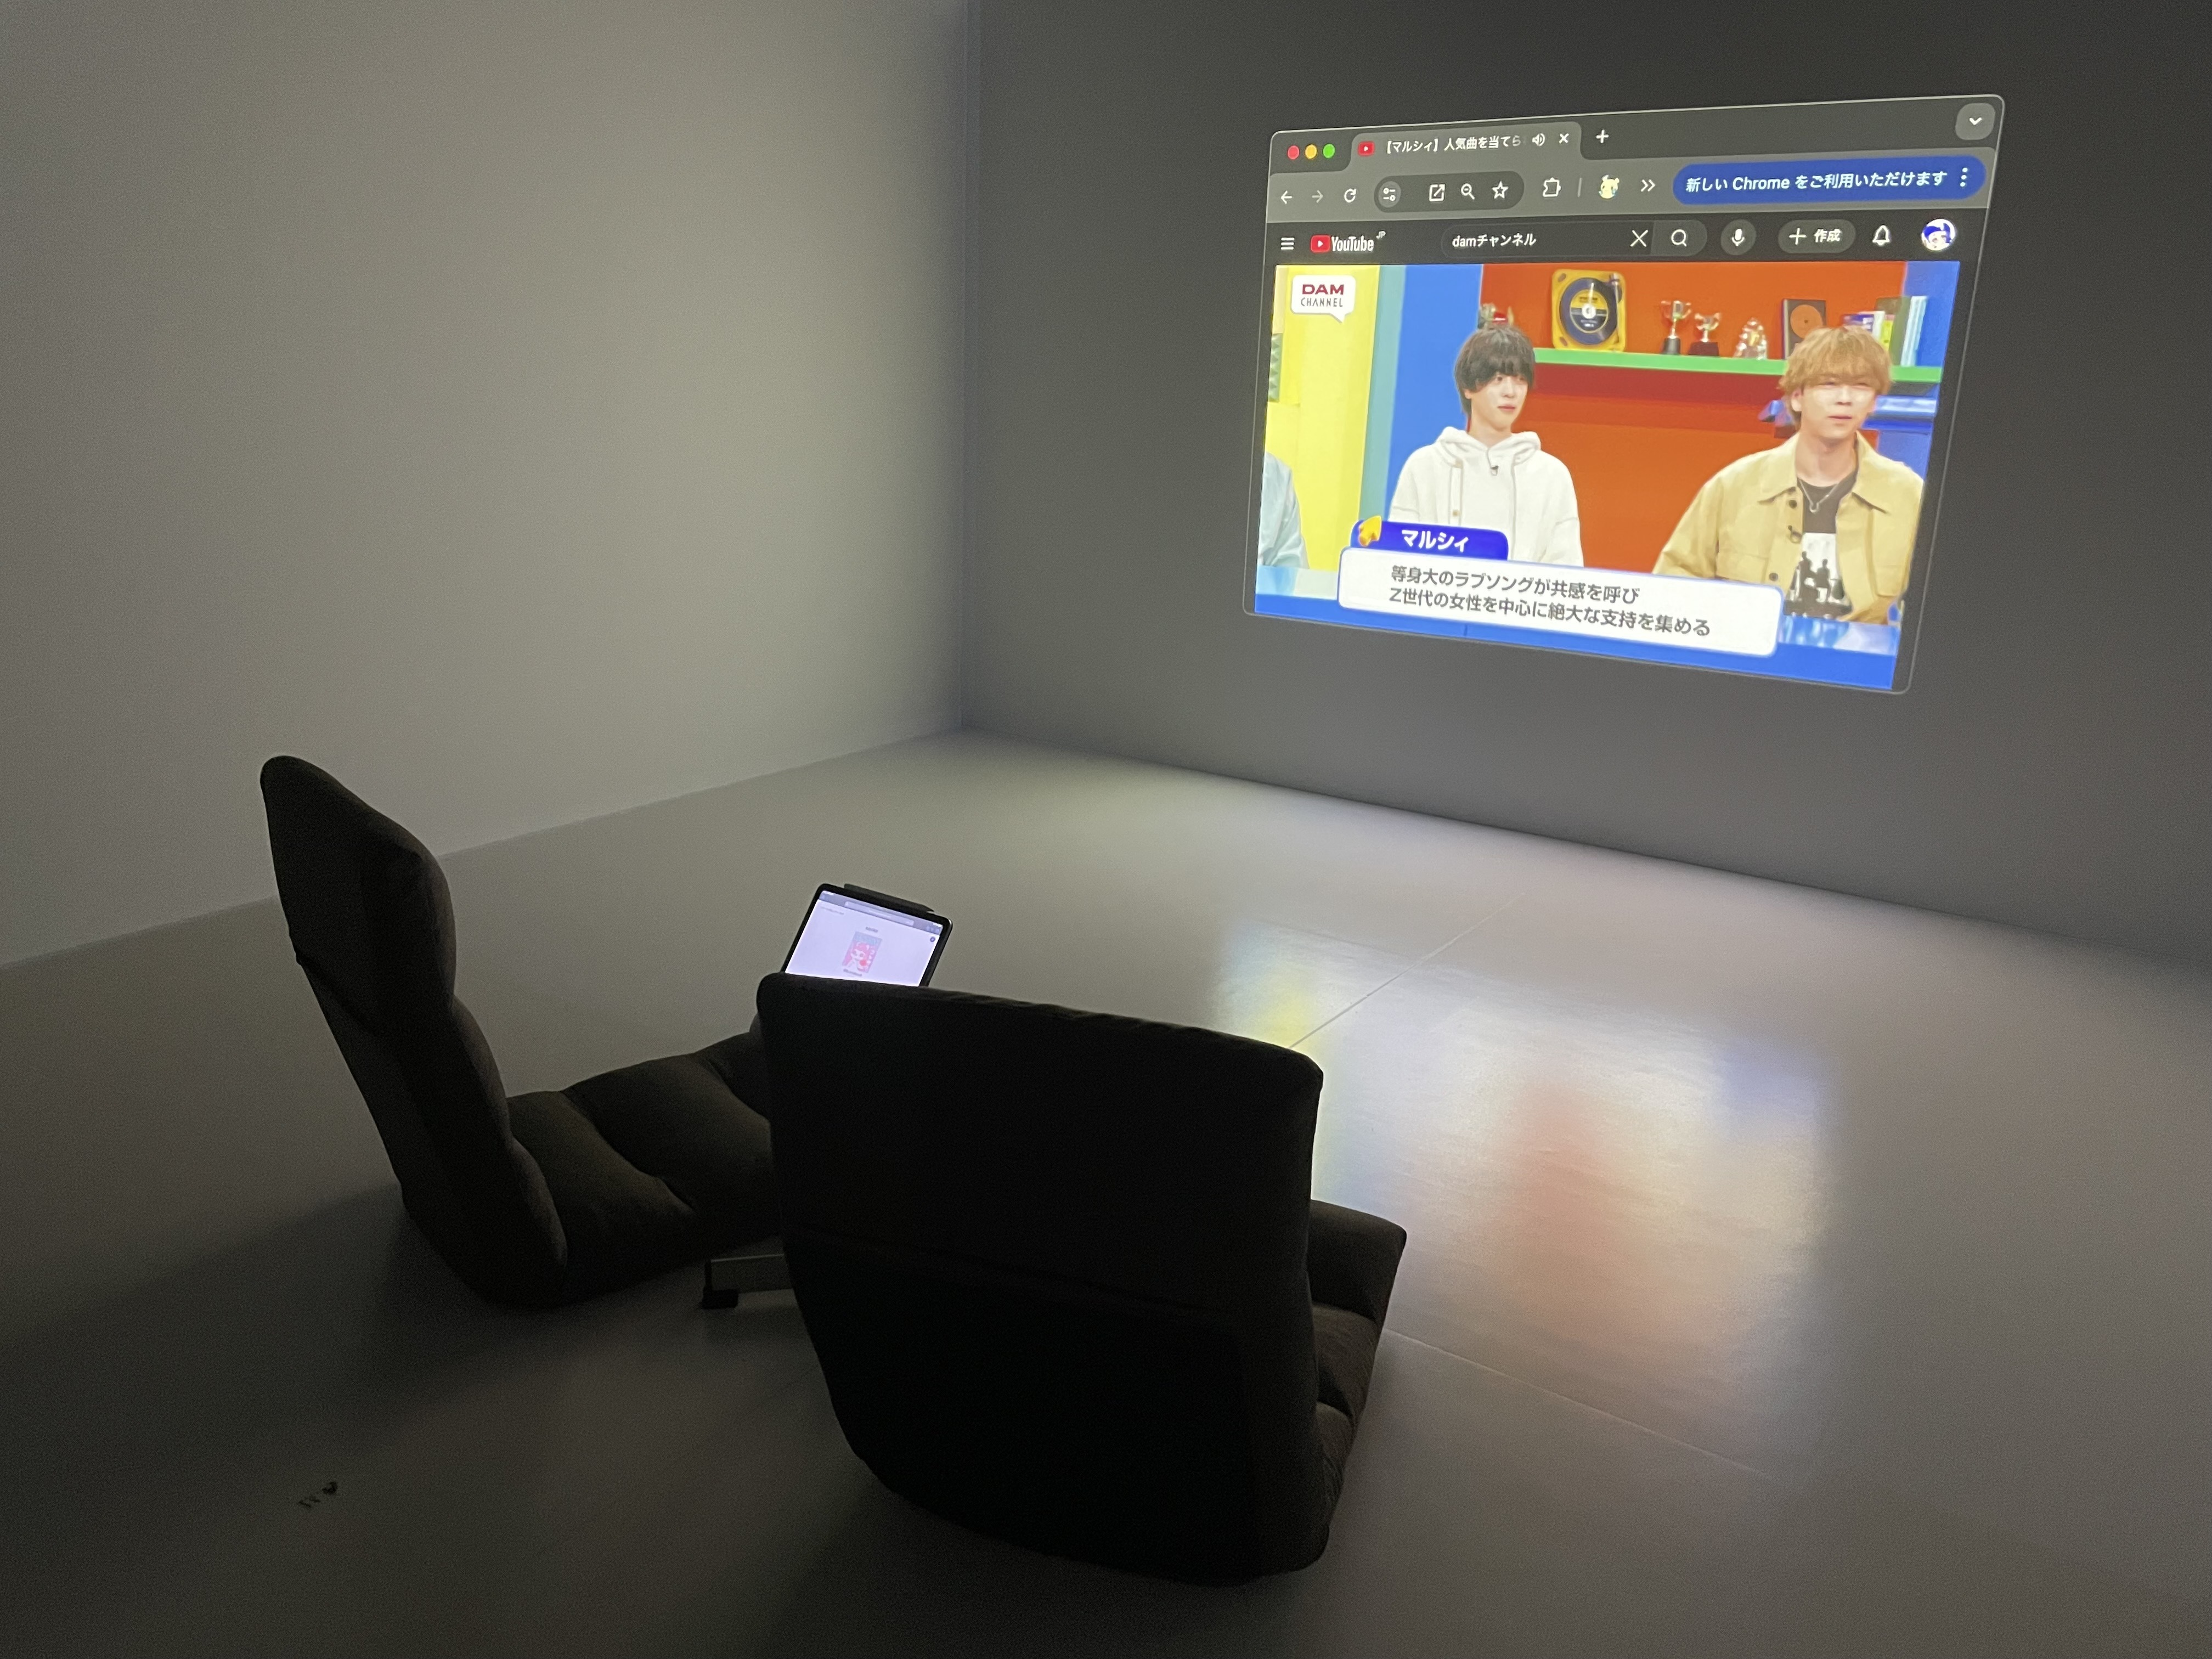
\includegraphics[width=0.75\linewidth]{image/実験環境.jpg}
    \caption{音楽共有セッションに用いる環境}
    \label{pic:実験環境}
\end{figure}


\subsubsection{実験参加者}
被験者は，年齢差がない学生・社会人の20名（18-24歳の男性8名，女性12名）を対象とし，10ペアで実験を行った．2群比較実験であるため，男女の比率が公平になるよう無作為に2群に割り当てた．

関係性は友人関係とした．友人関係とは，日常的な会話や活動を共にする程度でかつ，同じ空間で過ごしていても心理的負担を感じない関係性であり，自分の内面に関する深刻な悩み事を相談するほどの親密さには至っていない程度を対象とした．これは，初対面である場合は自己開示が重く感じられ，逆に親友レベルの関係性である場合はすでに深い自己開示を行えているため，友人という関係が最も適切であるとされている．


\subsection{実験手順}\label{実験手順}

音楽における自己開示の段階をレベル分けするため，選曲理由や楽曲にまつわる思い出の開示レベルを定義する．その後，このレベルに基づいて段階的に自己開示を促すシステムを実装する．

実験は事前準備と本実験の2段階で構成される．
事前準備では，被験者に50曲程度の「お気に入りの曲」プレイリストを作成してもらい，各楽曲に対する思い入れの強さを評価する．

本実験の音楽共有セッションでは，システムによる段階的な楽曲推薦を行う群（推薦あり群）と，支援を行わない群（推薦なし群）の2群で比較を行う．セッションは全8フェーズで構成され，各フェーズでは楽曲選択（推薦あり群はシステムが提示する候補から，推薦なし群は自身の作成したプレイリストの全楽曲から選択），楽曲再生，対話という流れで進行する．各フェーズ終了後，被験者は自己開示の度合いや楽曲体験の受容性に関する評価を行う．これらのデータを解析することで，段階的な自己開示が，相手の自己開示に対する受容性を向上させるかを検証する．

次節では，本実験で使用するシステムの設計・実装について詳しく説明する．
\section{自己開示を促す楽曲推薦システム}
本節では，システムの基本設計について述べる．

\begin{comment}
\subsection{要件}
選曲を通じた自己開示を促すには，システムに以下のような要件が必要である．

\subsection*{要件1. 個人の楽曲に対する自己開示レベルの定量化}
システムが自己開示を促進するうえでは，定量化する必要がある．

\subsection*{要件2. 段階的な自己開示の制御}
要件1で定量化した自己開示レベルについて，レベルの低い楽曲から高い楽曲へと段階的に開示を促す必要がある．

\subsection*{要件3. ユーザーの選曲過程や，受容度の変化を記録する}
要件2の段階的にシステムが提示した曲と，ユーザーの選択した曲の変化，すなわち要件1の自己開示レベルの変化を時系列的に記録できるシステムである必要がある．

\vskip\baselineskip

これらの要件を～．
\end{comment}

\subsection{3軸の分類基準}

本項では，\ref{3軸}項で整理した自己開示の3軸についての取得方法，定量化方法を検討する．「思い入れ」と「歌うことの自信」は，個人の主観であり，客観的指標として取得することが不可能である．そのため，主観指標として曲に対して表\ref{tab:evaluation_criteria}に示すように4段階で被験者に評価をさせることとした．

\begin{table}[htbp]
\centering
\caption{楽曲の評価基準}
\label{tab:evaluation_criteria}
\begin{tabular}{|c|c|c|}
\hline
評価値 & 思い入れ & 歌うことの自信 \\
\hline
1 & ほとんど思い入れがない & ほとんど自信がない \\
2 & あまり思い入れがない & あまり自信がない \\
3 & やや思い入れがある & やや自信がある \\
4 & とても強い思い入れがある & とても自信がある \\
\hline
\end{tabular}
\end{table}

楽曲の人気度については，個々人間で知っている/知らない曲を完全に網羅することは難しく，人により曲の認知度は違って感じられるため，主観指標を使うことは難しい．そのため，Spotify Web API\cite{SpotifyWebAPI}から取得できるpopularityという客観的な数値（0-100）を使用する．これら3つの指標に基づき，各楽曲の自己開示レベルを定量的に評価する．

次項では，各軸の数値から自己開示レベルを決定する方法について述べる．


\subsection{自己開示レベルの区分}

\ref{3軸}項での3軸に基づき，カラオケにおける自己開示を4つのレベルに分類する．既存の研究ではこのような自己開示の段階を定義した手法は存在しない．そのため，今回は各軸の値を活かすため，2分法を用いて表\ref{tab:自己開示レベルの分類}のように分類を行うこととした．

思い入れと歌うことの自信は，表\ref{tab:evaluation_criteria}の4段階評価から，1-2の値を低い，3-4を高いとする．人気度については，Spotify APIから取得した1-100の値を，50を閾値として高低の2値に変換する．なお，思い入れが低く（1-2），歌唱への自信も低く（1-2），人気度も低い（50未満）楽曲については，開示者の感情表現も乏しく，被開示者からの受容も得られにくいことから適切に機能しないと判断し，分類から除外する．
% この分類では，思い入れを主軸とし，歌唱への自信と人気度を補助的な要素として扱う．

\begin{table}[H]
\centering
\caption{自己開示レベルの分類}
\begin{tabular}{|c|c|c|c|}
\hline
自己開示レベル & 思い入れ & 歌える自信 &  人気度  \\
\hline
1 & ない & ある & 高い \\
\hline
1 & ない & ない & 高い \\
\hline
2 & ない & ある & 低い \\
\hline
2 & ある & ある & 高い \\
\hline
3 & ある & ない & 高い \\
\hline
3 & ある & ある & 低い \\
\hline
4 & ある & ない & 低い \\
\hline
- & ない & ない & 低い \\
\hline
\end{tabular}
\label{tab:自己開示レベルの分類}
\end{table}


\subsection{実装}
提案したシステム設計に基づき，Webアプリケーションとして実装を行った．本項では，使用した開発環境，事前準備と本実験のデータフローについて説明する．

\vskip.5\baselineskip

システムの実装には，表\ref{tab:libraries}に示すライブラリとフレームワークを使用した．アプリケーションのベースとしてNode.js 20.17.0を採用し，フロントエンド・バックエンドの統合フレームワークとしてNext.js\cite{NextJS}を使用した．
データベースにはSupabase\cite{Supabase}を採用し，データベース管理を行った．また，楽曲情報の取得にはSpotify Web APIを利用し，next-authとiron-sessionを用いてAPI認証を実装した．
本アプリケーションは実験被験者が実際に使用することを想定し，安定した運用環境としてVercel\cite{Vercel}を使用した．


\begin{table}[H]
\caption{システム作成に使用したライブラリ・バージョン}
\label{tab:libraries}
\begin{center}
\begin{tabular}{|l|c||l|c|} \hline
\multicolumn{4}{|c|}{Node.js 20.17.0} \\ \hline
ライブラリ & バージョン & ライブラリ & バージョン \\ \hline
@mui/material & 6.3.1 & @supabase/supabase-js & 2.47.10 \\
axios & 1.7.9 & iron-session & 8.0.4 \\
next & 15.1.3 & next-auth & 4.24.11 \\
react & 19.0.0 & tailwindcss & 3.4.1 \\
typescript & 5.7.2 & & \\ \hline
\end{tabular}
\end{center}
\end{table}

\ref{実験手順}項の実験手順を満たすような事前準備のデータフローを図\ref{fig:事前準備のデータフロー}に，本実験の音楽共有セッションでのデータフローを図\ref{fig:音楽共有セッションのデータフロー}に示す．

\begin{figure}[H]
    \centering
    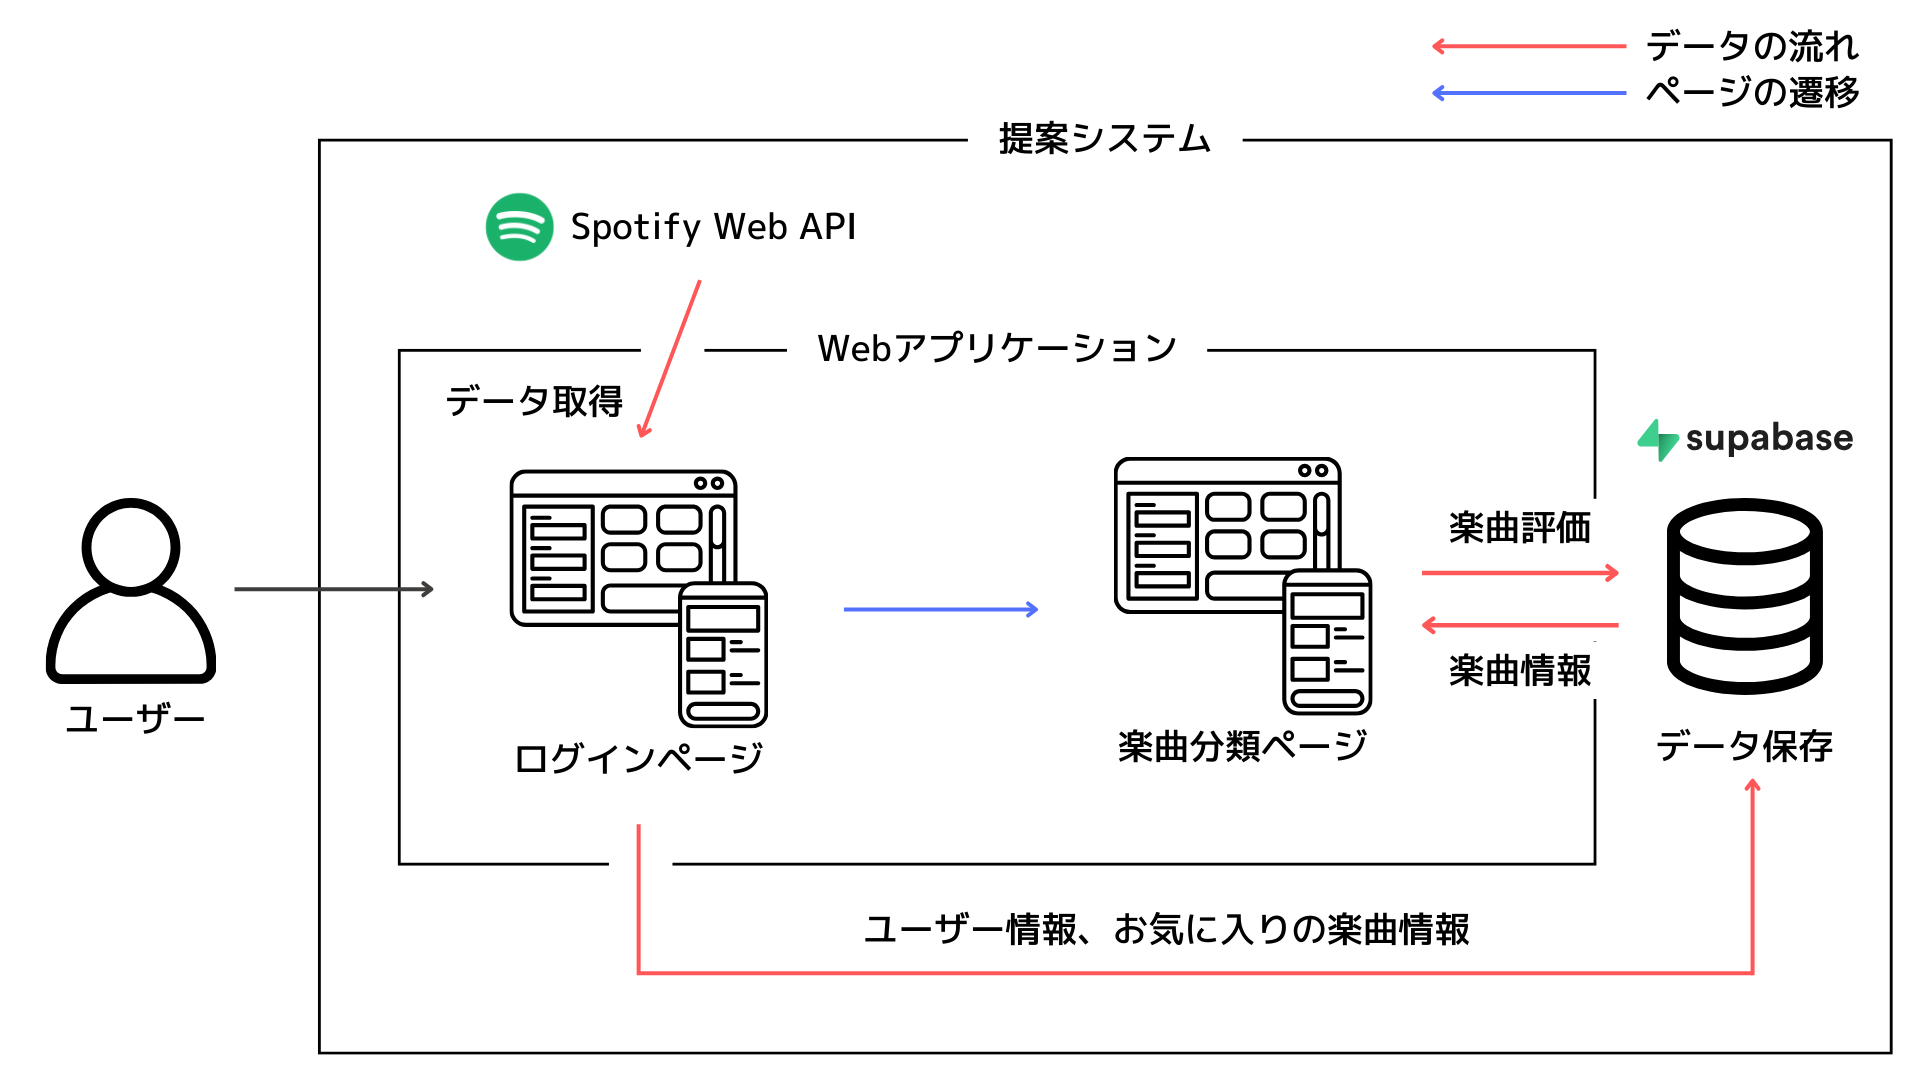
\includegraphics[width=1\linewidth]{image/data-flow-chart1.png}
    \caption{事前準備のデータフロー}
    \label{fig:事前準備のデータフロー}
\end{figure}

\begin{figure}[H]
    \centering
    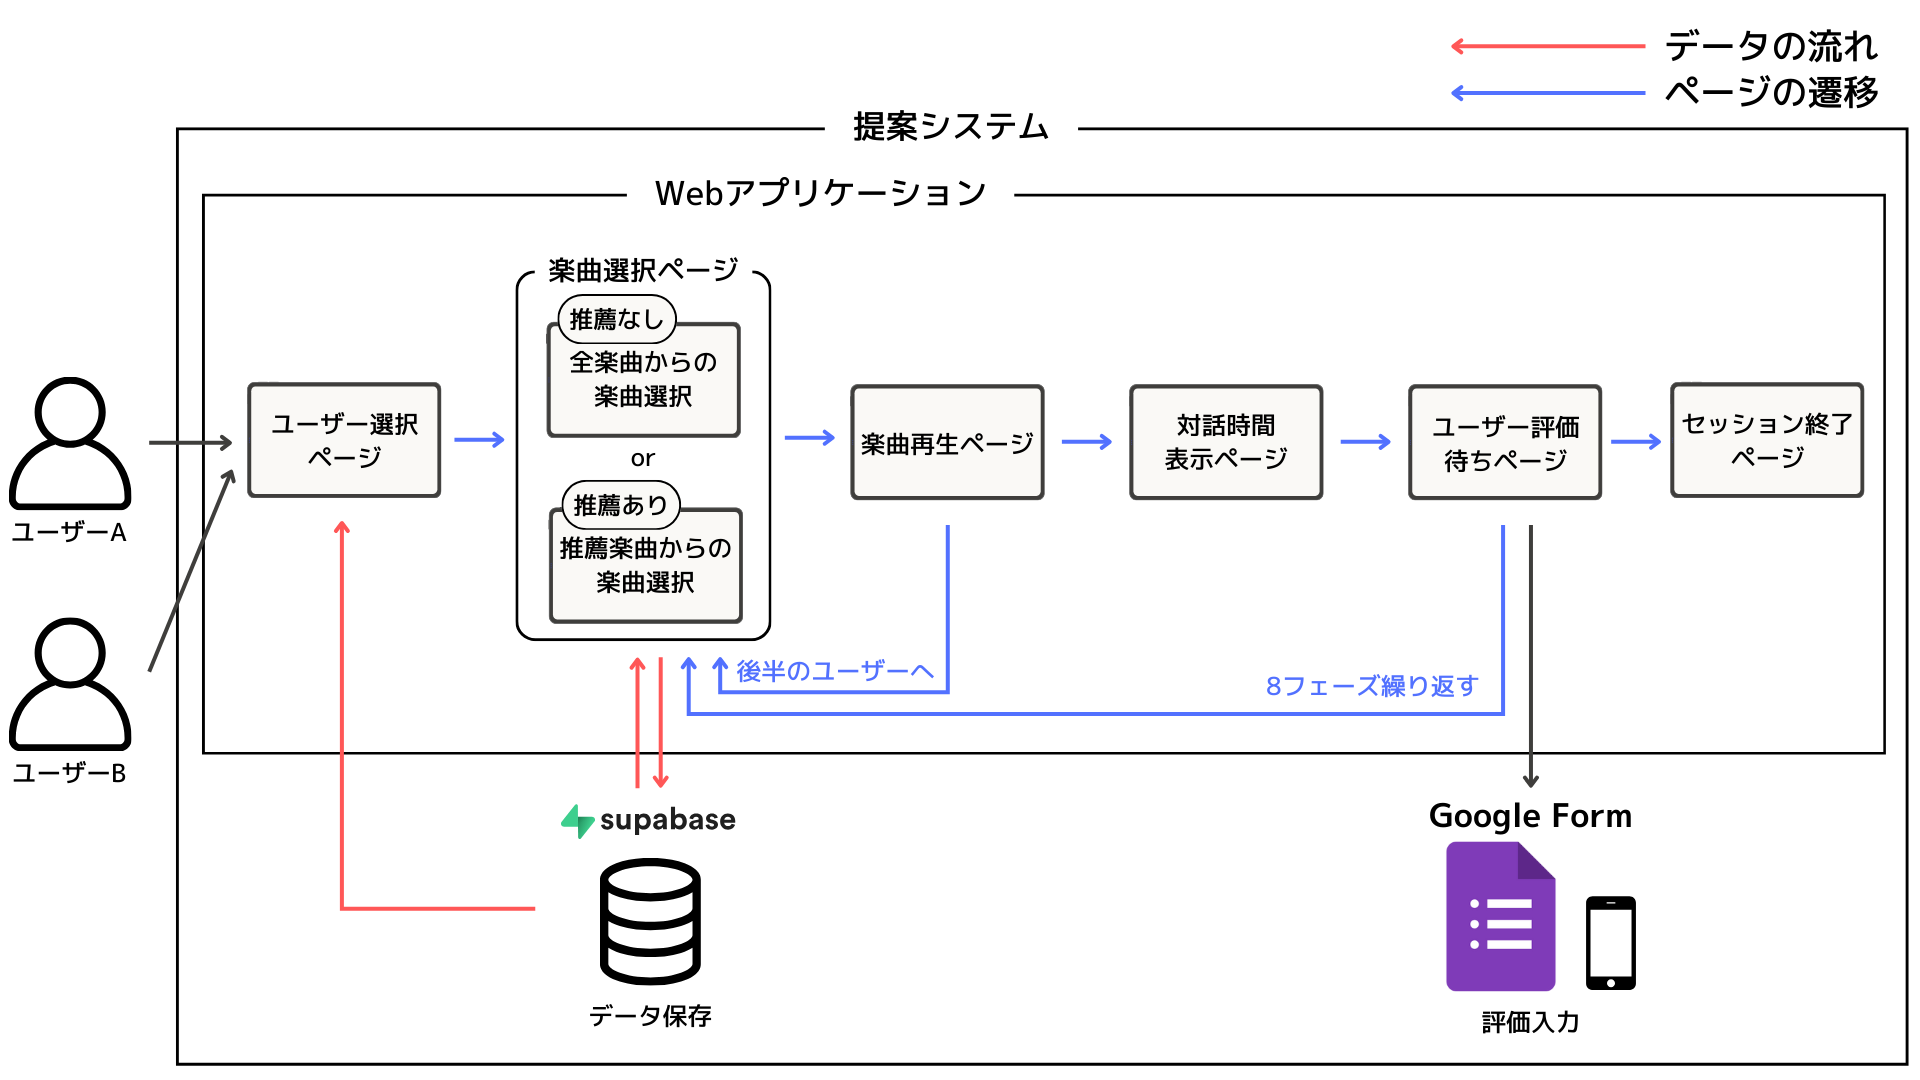
\includegraphics[width=1\linewidth]{image/data-flow-chart2.png}
    \caption{音楽共有セッションのデータフロー}
    \label{fig:音楽共有セッションのデータフロー}
\end{figure}

\section{実験方法}
実験は事前準備と本実験の2段階で構成される．
本実験では，システムによる段階的な楽曲推薦を行う群（推薦あり群）と，支援を行わない群（推薦なし群）の2群で比較を行う．

\subsection{事前準備}

事前準備では，被験者に実験用のSpotifyアカウントを作成してもらい，50曲程度の「お気に入りの曲」プレイリストを作成する．その後，Webアプリケーションを用いて，図\ref{fig:song_classification}に示した楽曲分類画面で，各楽曲に対する思い入れの強さと歌唱への自信を4段階で評価する．ユーザーの作業の負担を考慮し，楽曲分類の際には途中で保存ができる機能を実装した．

また，図\ref{fig:classified_songs}に分類済みの楽曲一覧を確認できる画面を示す．この画面では，分類が完了した楽曲の一覧を表示する．被験者は，自身が分類した楽曲を確認することができる．また，再度の分類もできるようにした．

\begin{figure}[H]
   \centering
   \begin{minipage}[b]{0.45\linewidth}
       \centering
       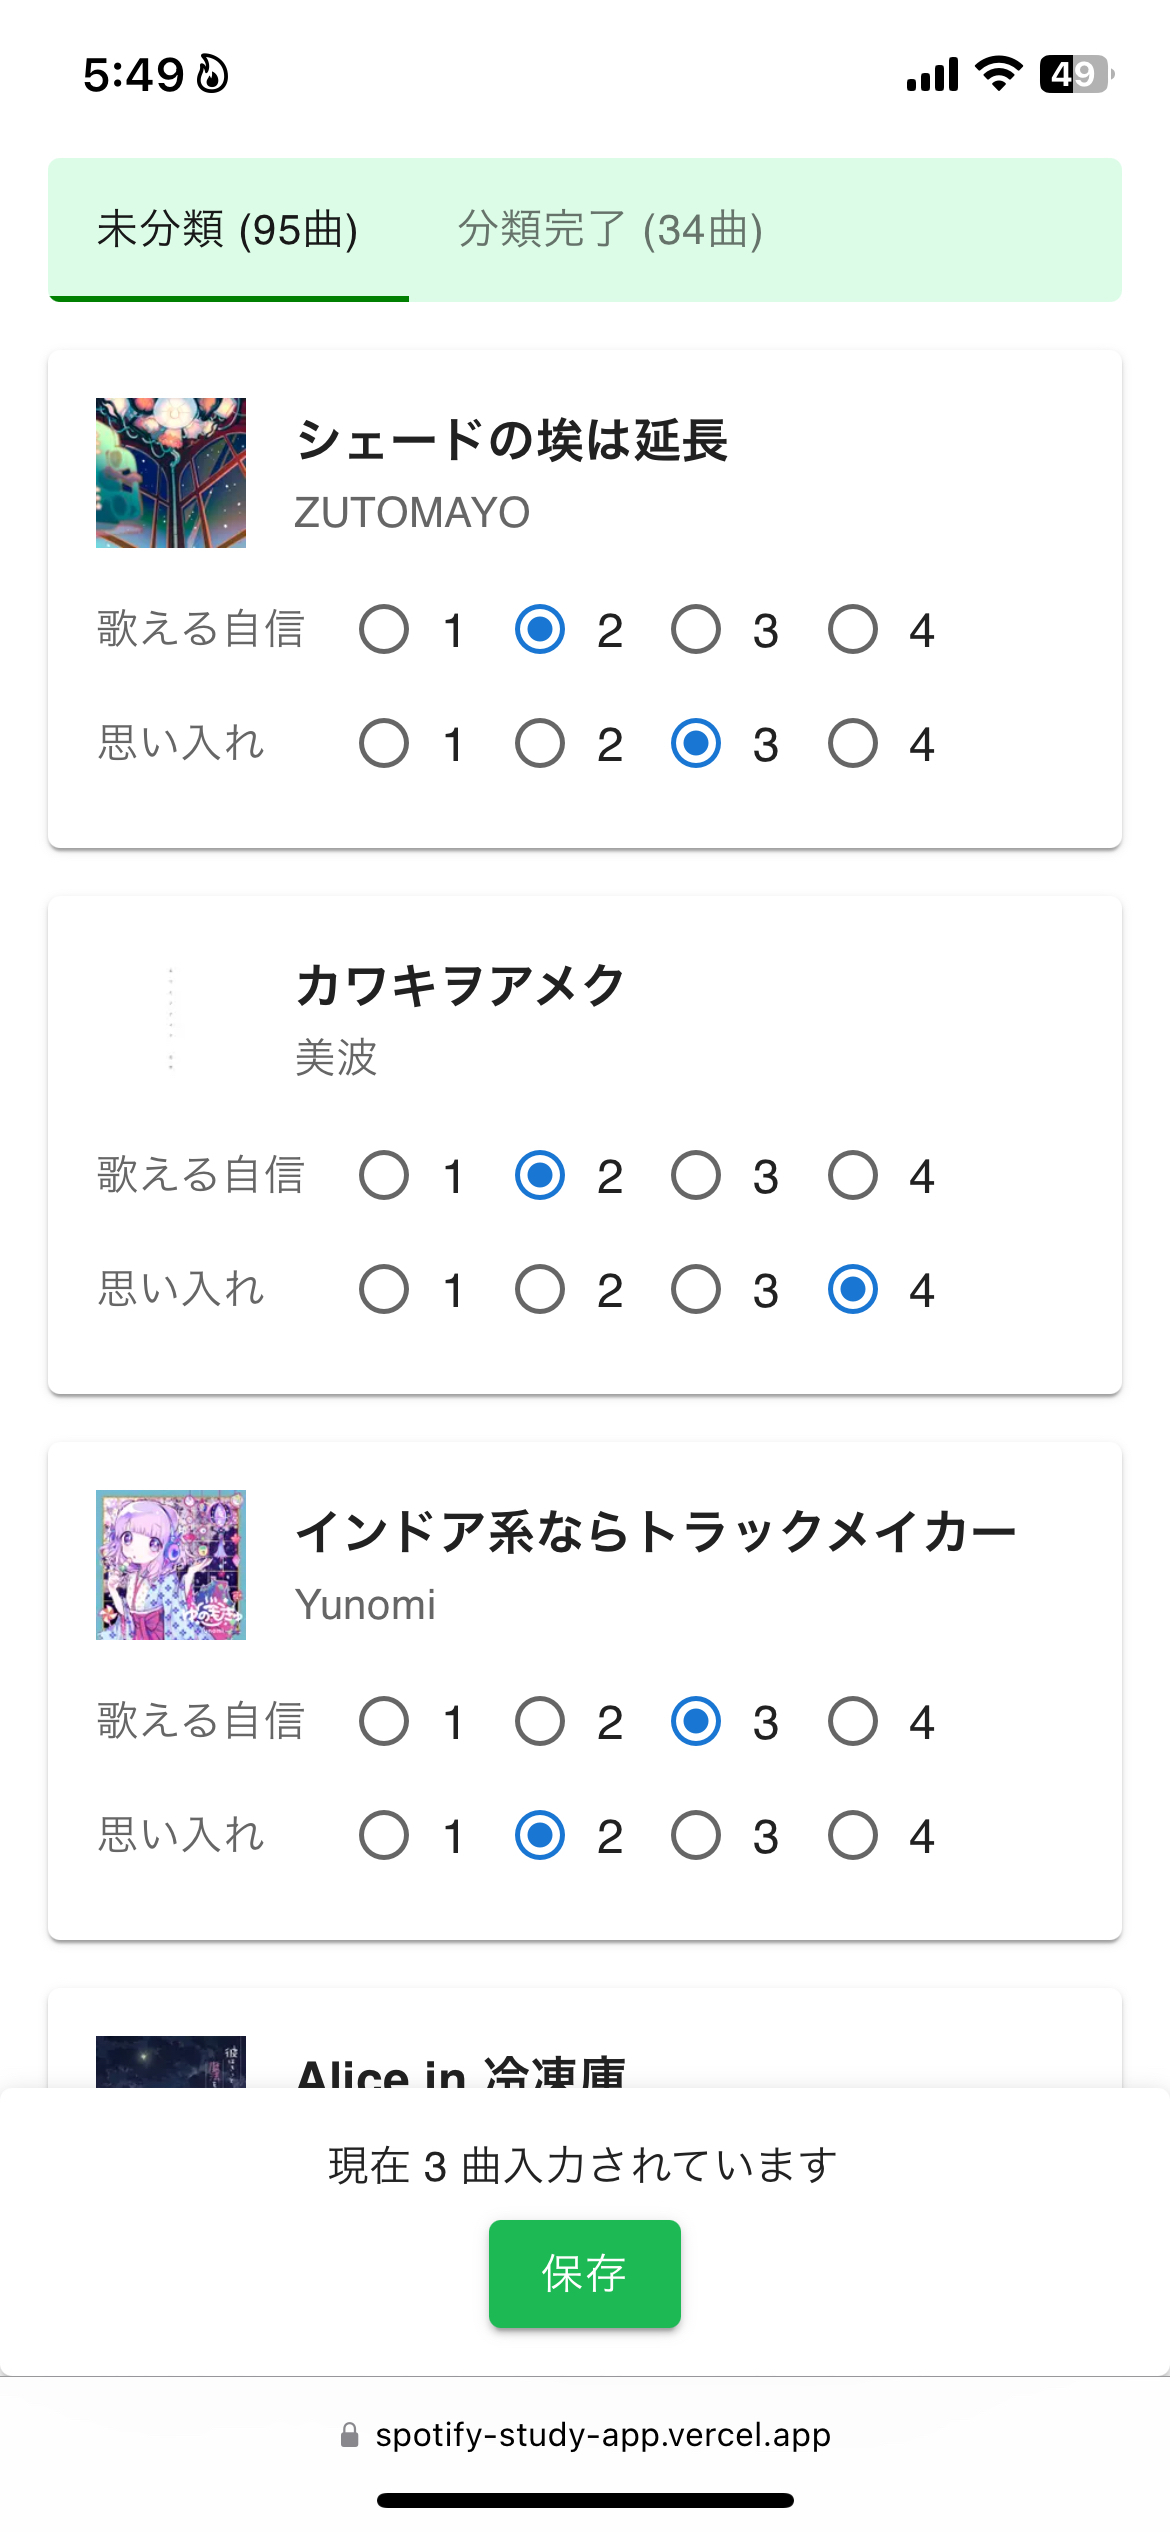
\includegraphics[width=0.9\linewidth]{image/ss_未分類.png}
       \caption{楽曲分類画面}
       \label{fig:song_classification}
   \end{minipage}
   \hfill
   \begin{minipage}[b]{0.45\linewidth}
       \centering
       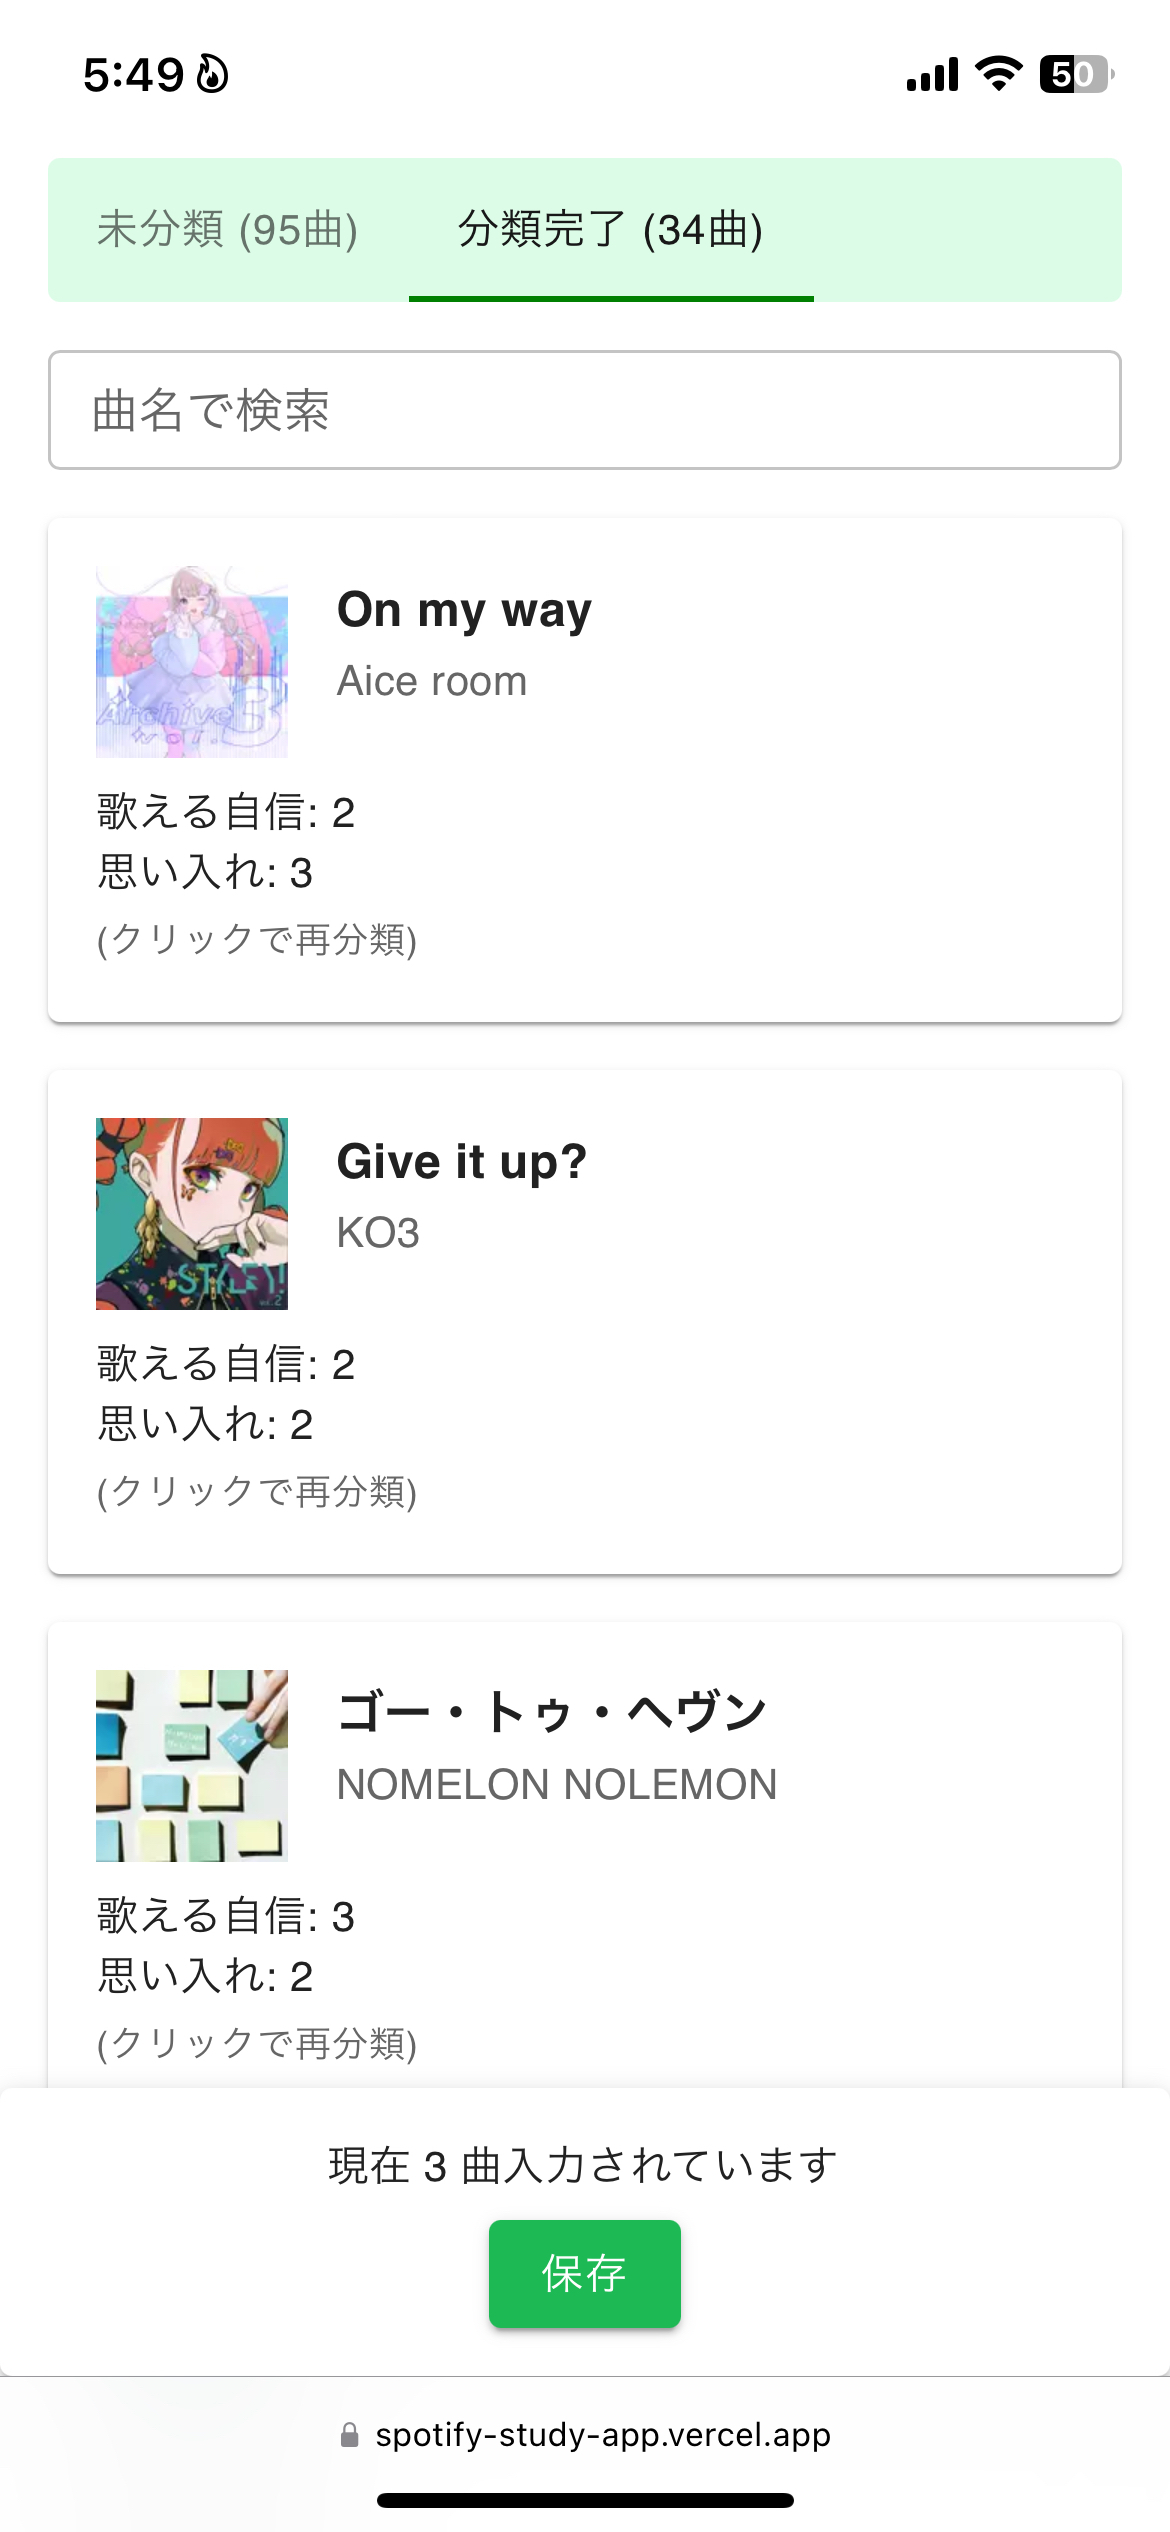
\includegraphics[width=0.9\linewidth]{image/ss_分類済み.png}
       \caption{分類済み楽曲一覧画面}
       \label{fig:classified_songs}
   \end{minipage}
\end{figure}


\subsection{本実験}

各被験者ペアを，本学の実験環境に案内し，互いに横並びになる形で座椅子に着席させる（図\ref{pic:実験環境}参照）．被験者に対して実験手順と注意点について説明し，音楽共有セッションを開始するよう指示をする．音楽共有セッションについては，以下の説明を行う．

\vskip.5\baselineskip

\textbf{推薦なし群:}
このセッションでは，あなたの音楽の好みについて相手と共有していただきます．
好きな曲をリストから選んで，選んだ曲を一緒に聴いたあと，その曲についてお話しください．曲にまつわる思い出や感想など，自由に会話を楽しんでください．

\vskip.5\baselineskip

\textbf{推薦あり群:}
このセッションでは，音楽を通じたコミュニケーションを体験していただきます．
システムが，あなたの音楽の興味や好みに基づいた曲の候補を提示します．
提示された候補の中から，共有したい曲を選んでください．
選んだ曲を一緒に聴いたあと，その曲についてお話しください．曲にまつわる思い出や感想など，自由に会話を楽しんでください．

\vskip.5\baselineskip

音楽共有セッションは全8フェーズで構成される．各フェーズは2ターン制を採用しており，以下の流れで進行する：

\begin{itemize}
    \item 第1ターン：被験者Aが開示者となり，被験者Bが被開示者となる
    \item 第2ターン：被験者Bが開示者となり，被験者Aが被開示者となる
\end{itemize}

つまり，1フェーズは「被験者A→被験者B」「被験者B→被験者A」という順序で2回の自己開示が行われる．

各ターンは，以下の3つのステップにより構成される．

\begin{enumerate}
    \item 楽曲選択フェーズ（30秒）
    \begin{itemize}
        \item 推薦なし群：事前に作成した個人のプレイリストから任意の1曲を選択する（図\ref{fig:free_selection}）
        \item 推薦あり群：システムが推薦する4曲の中から1曲を選択する（図\ref{fig:recommendation}）
    \end{itemize}
    
    \item 楽曲再生フェーズ（30秒）
    \begin{itemize}
        \item 選択楽曲を再生する．開示者が好きな場所から再生することができる
    \end{itemize}
    
    \item 対話フェーズ（60-90秒）
    \begin{itemize}
        \item 選曲理由や楽曲にまつわる思い出などを自由に共有し対話する
    \end{itemize}
    
\end{enumerate}

1フェーズが終わるごとに，GoogleForms\cite{googleforms}を利用して開示者と被開示者の双方が評価を行う．

\vskip.5\baselineskip

\begin{figure}[H]
    \centering
    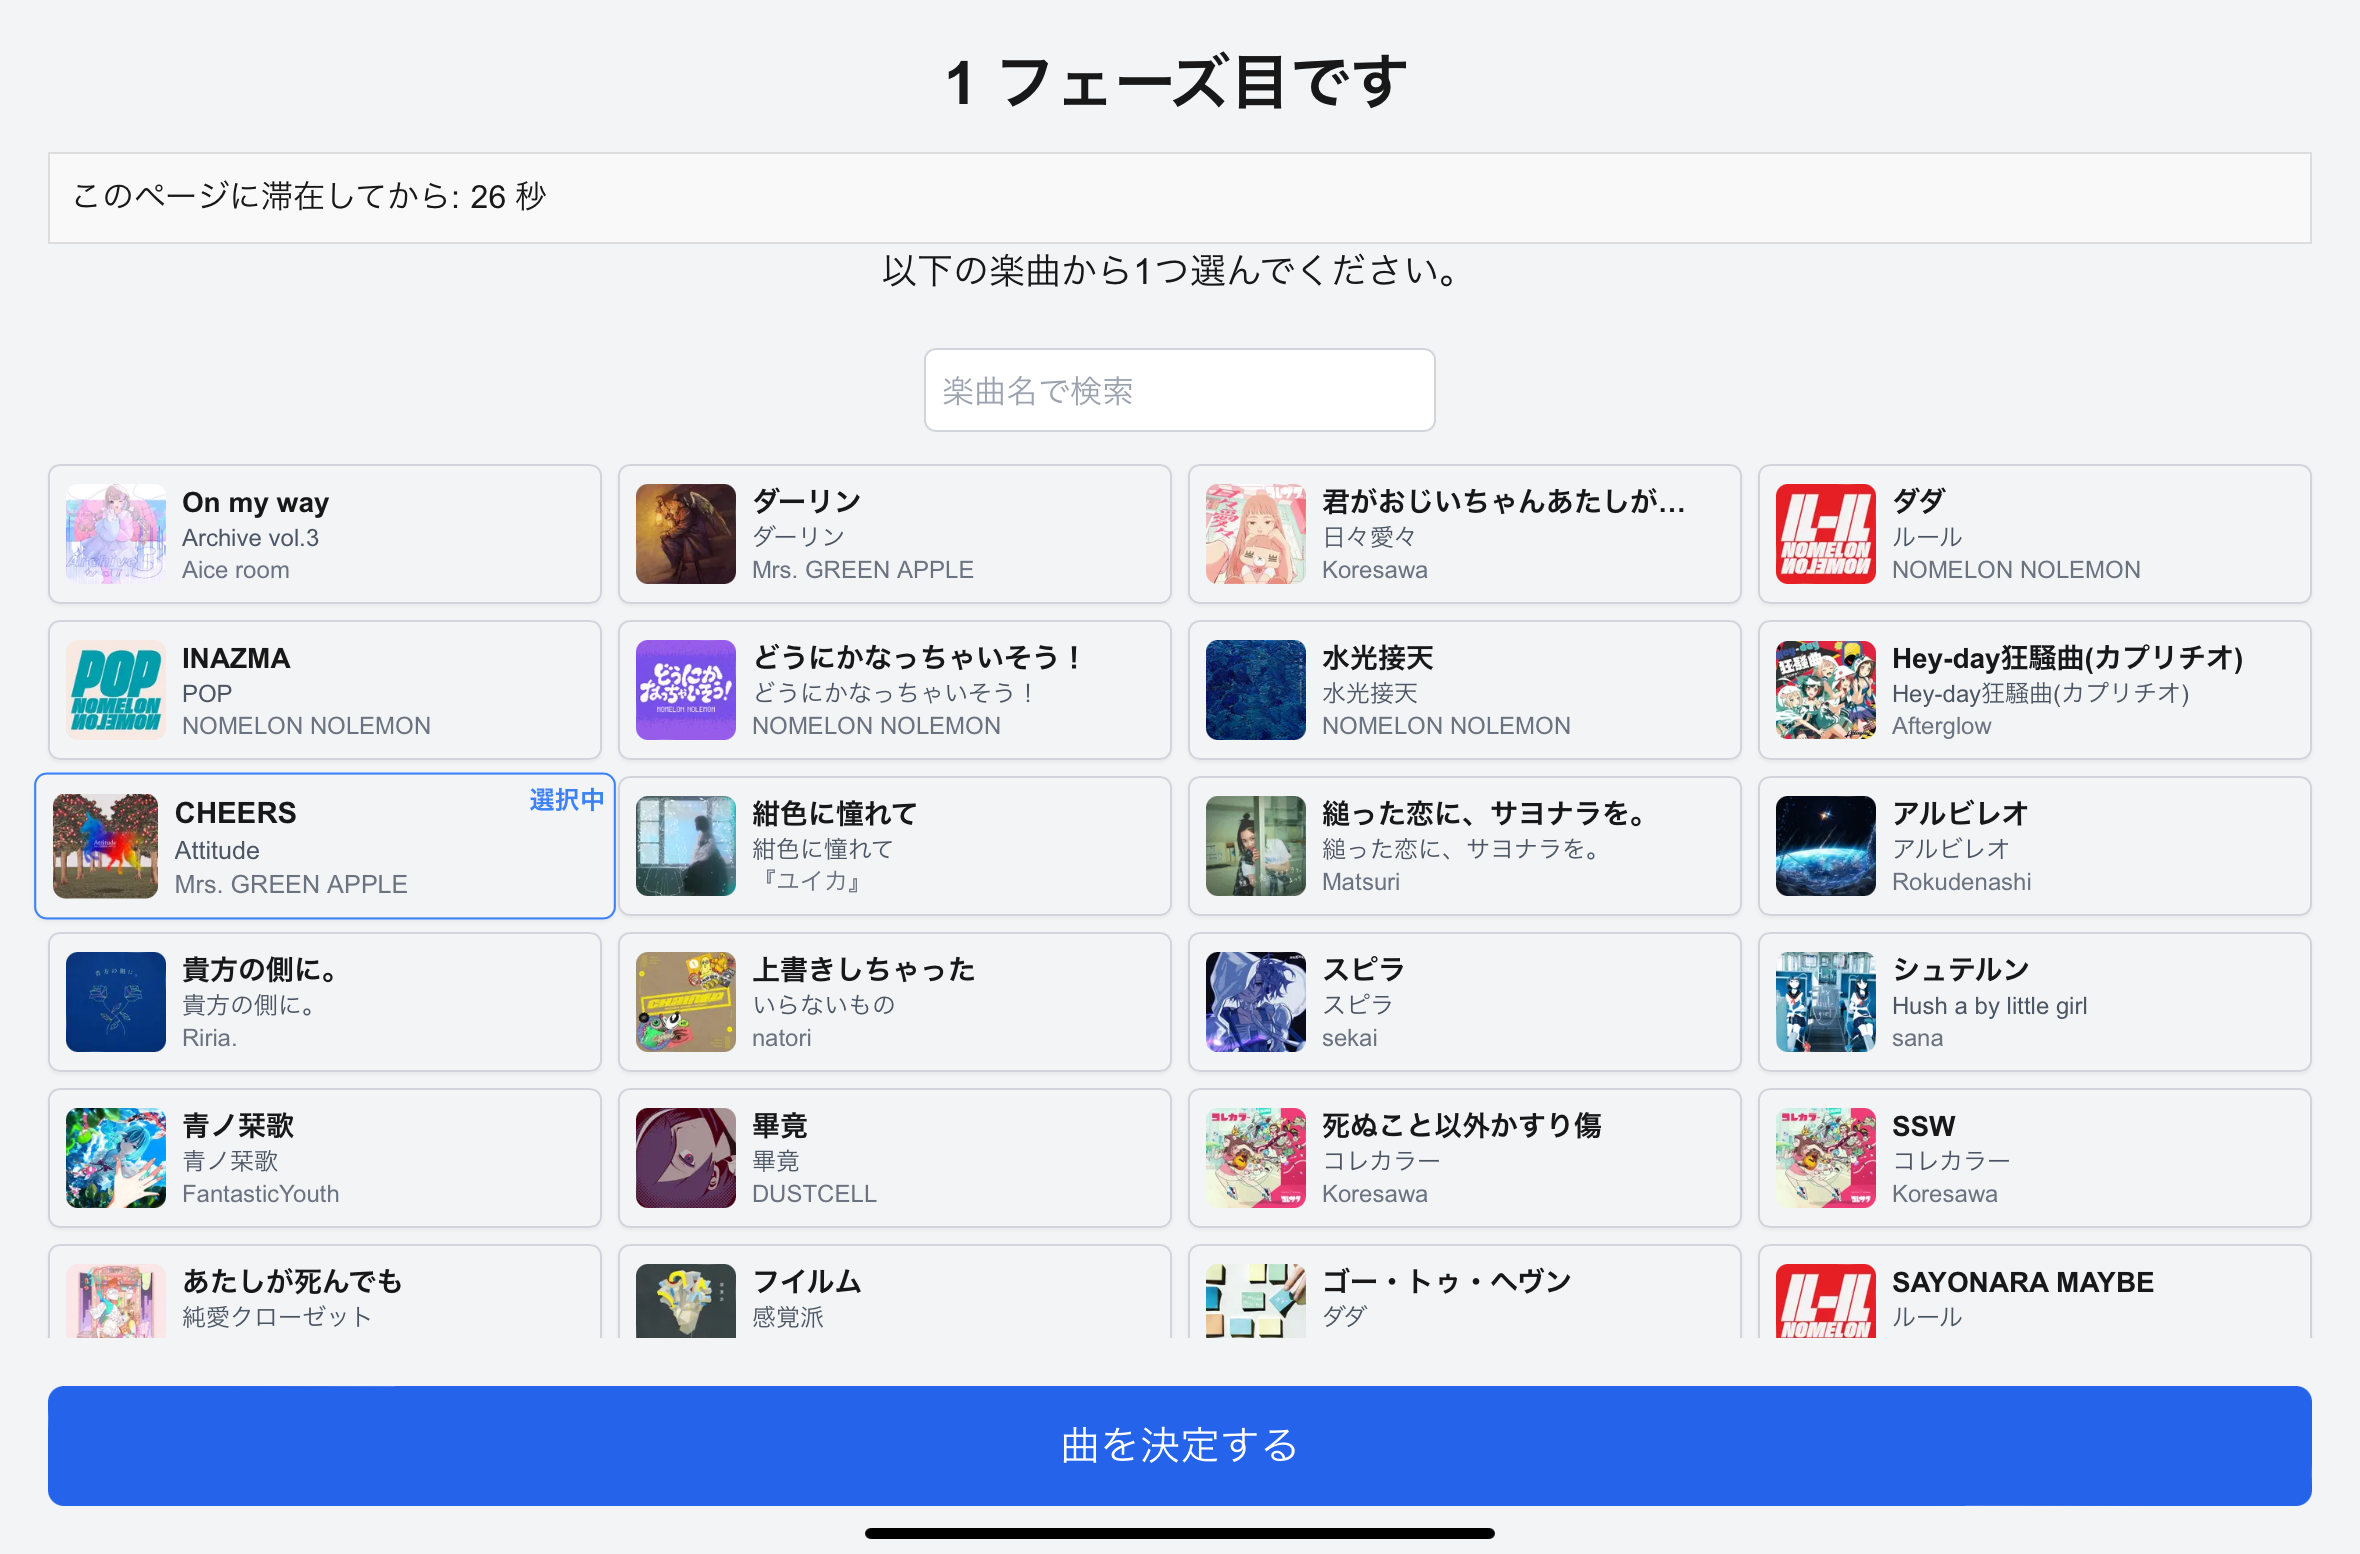
\includegraphics[width=0.9\linewidth]{image/ss_推薦なし_選曲.png}
    \caption{自由選択画面（推薦なし群）}
    \label{fig:free_selection}
\end{figure}

\begin{figure}[H]
    \centering
    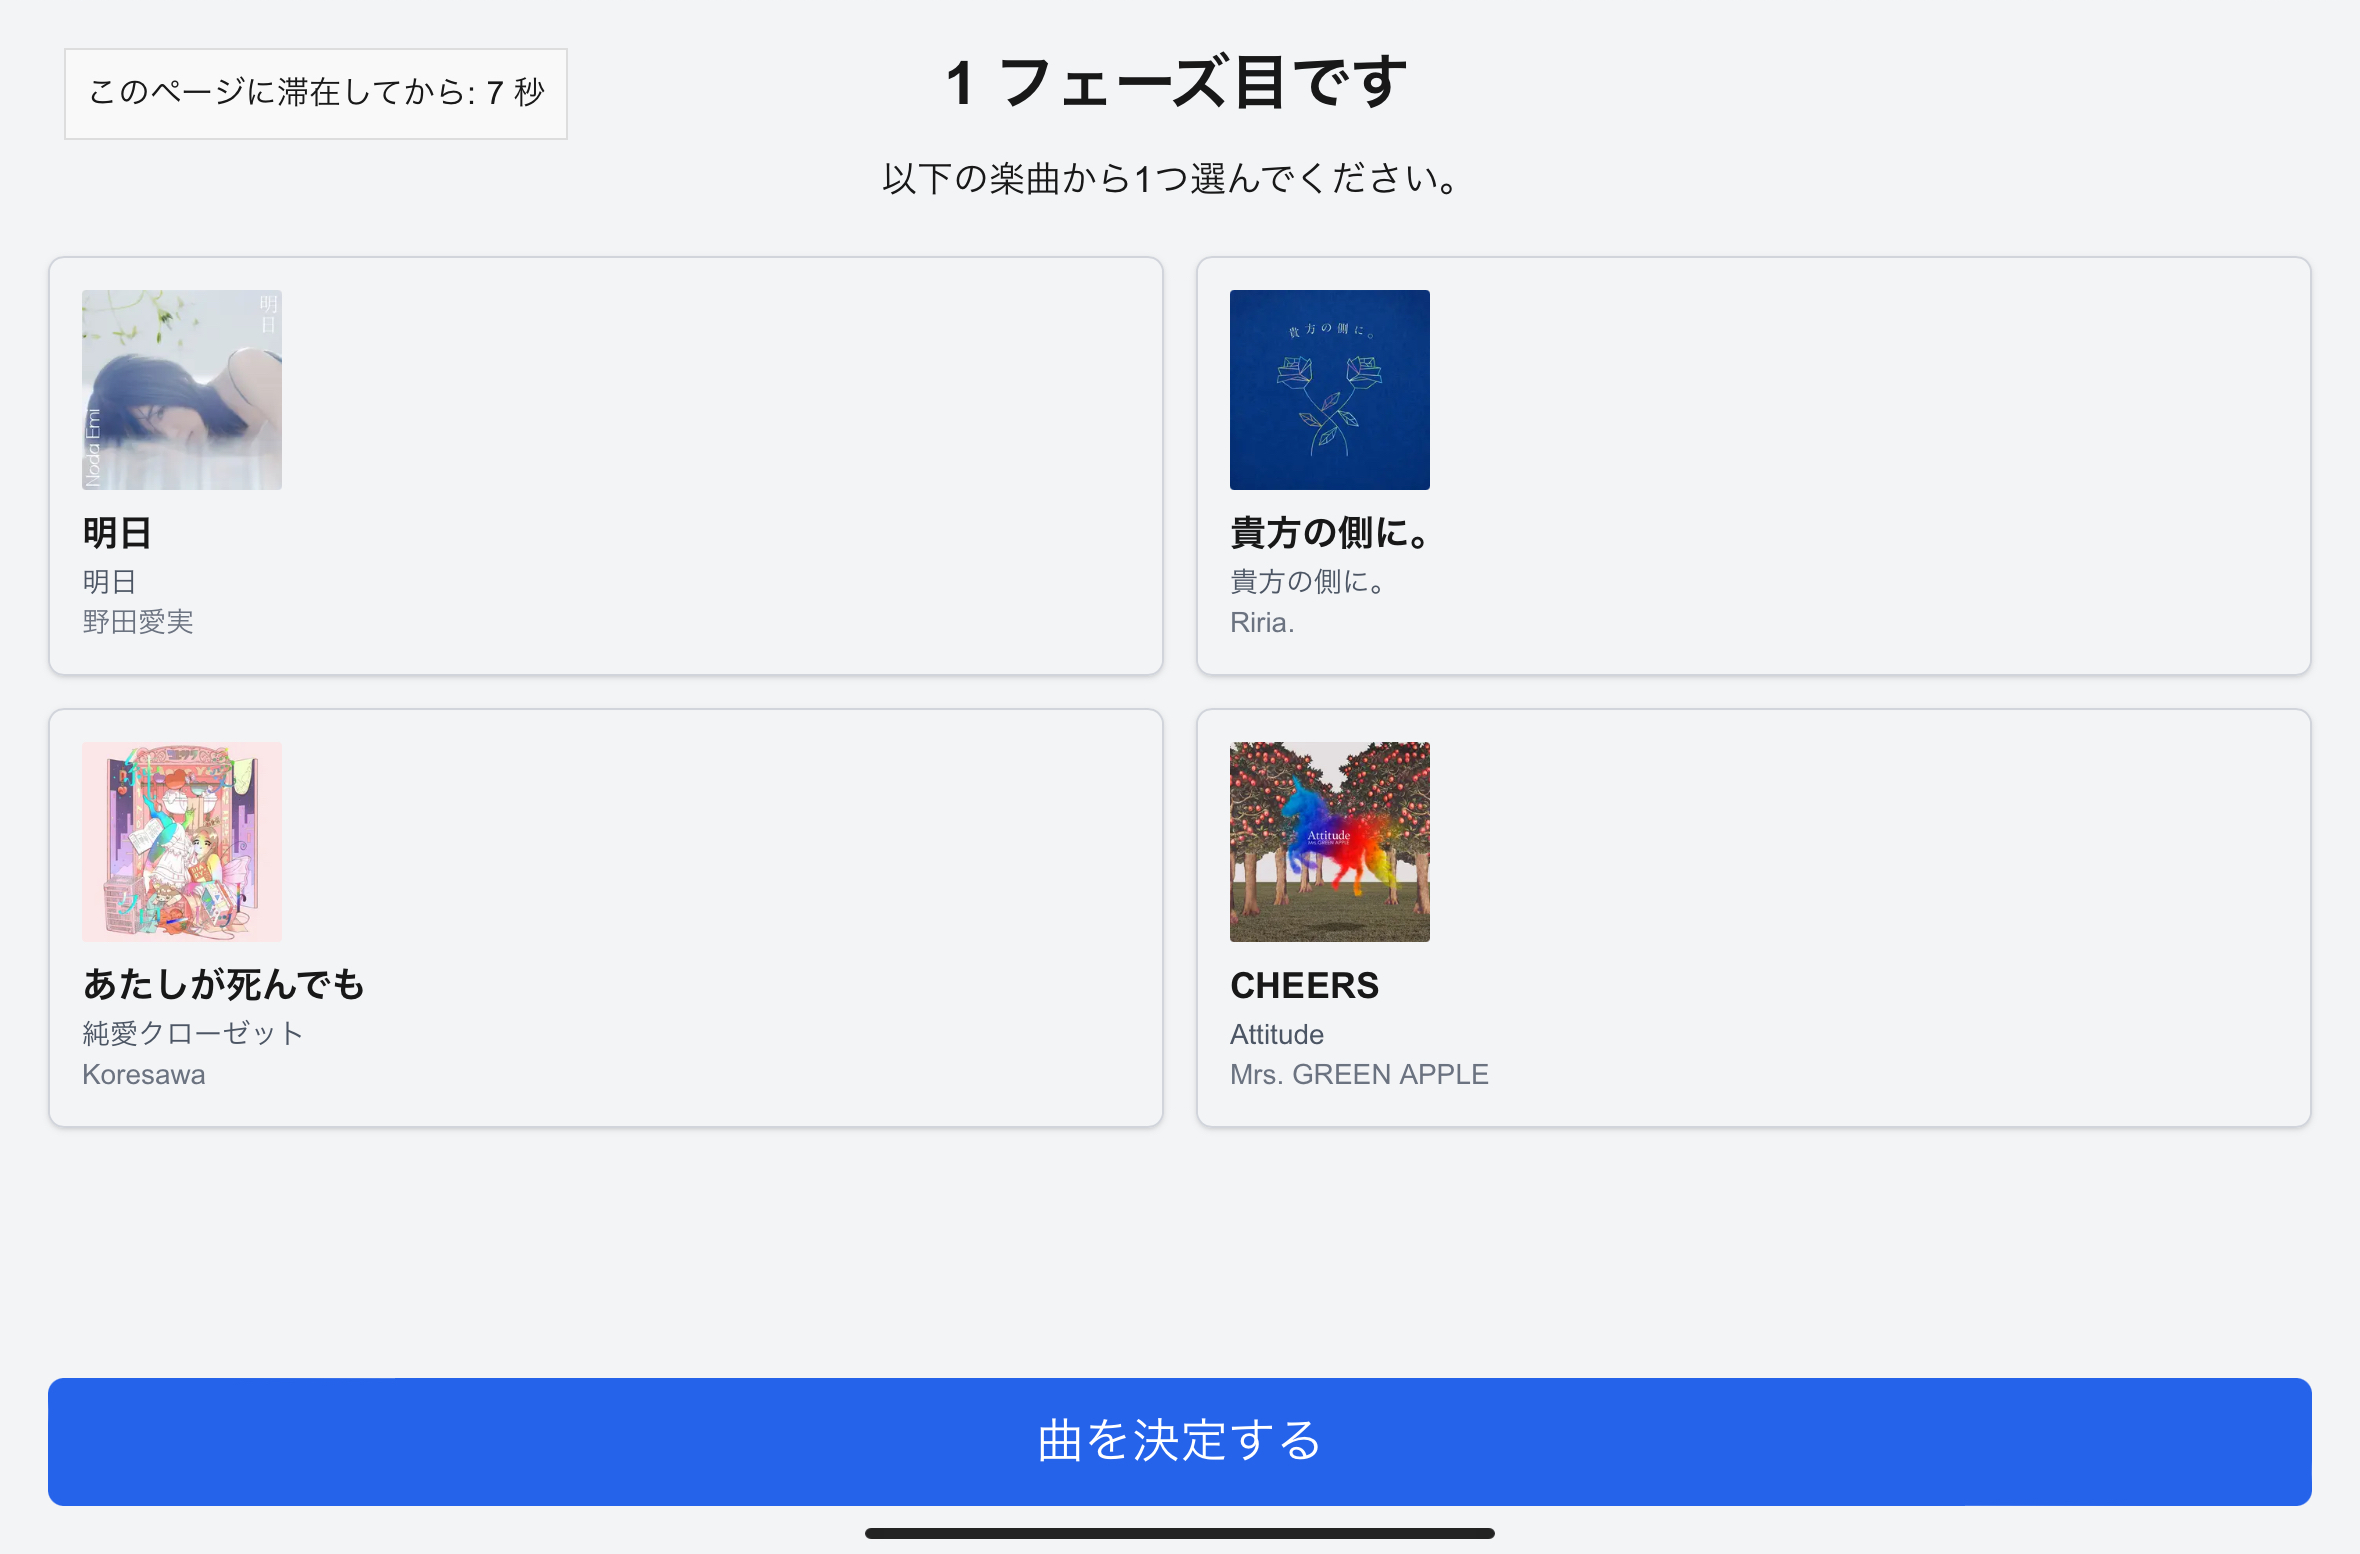
\includegraphics[width=0.9\linewidth]{image/ss_推薦あり_選曲.png}
    \caption{楽曲推薦画面（推薦あり群）}
    \label{fig:recommendation}
\end{figure}


% \subsection*{注意点}
% あとでくわしくかく

\section{評価方法}

\ref{研究課題と仮説}節で述べた仮説を検証するため，実験を実施するうえで以下の4つの指標について評価を実施する．

\vskip.5\baselineskip

\textbf{自己開示レベル:}自己開示のレベルの推移を明らかにするため，システムログより，各フェーズでの選曲履歴を取得する．
\vskip.5\baselineskip

\textbf{受容度:}仮説1, 2を検証するため，受容性の評価は，被開示者側と開示者側の両面から測定を行う．表\ref{実験中のアンケート項目}に，実験中のアンケート項目を示す．被開示者に対して，相手の自己開示をどの程度理解し，受け入れることができたかについて，表\ref{実験中のアンケート項目}のEQ1, EQ2を使用する．また，開示者側が知覚した相手からの受容についても取得することとして表\ref{実験中のアンケート項目}のEQ5, EQ6を使用する．これにより，段階的な自己開示が受容性に与える効果を，定量的に分析することができる．

また，実験終了後に相手の自己開示に対する印象や，理解が深まった点について表\ref{実験後のアンケート項目}のアンケートを行う．具体的には，相手に対する理解度，相手の音楽の好みに対する理解度，今後も相手と音楽を通じた会話をしたいと思うかを評価項目として設定する．
\vskip.5\baselineskip

\textbf{曲への興味:}仮説2を検証するため，被開示者に対し，選択された楽曲を知っていたかどうか（EQ3）と，相手の曲に興味を持てたかどうか（EQ4）という指標で相手の選曲に対しての評価を行う．これにより，音楽への興味度と受容性の関係性を分析する．
\vskip.5\baselineskip

\textbf{被験者の意見:}実験後のヒアリング項目を表\ref{実験後のヒアリング項目}に示す．選曲の意識，セッション全体の雰囲気，フェーズ前半と後半での違いなどについて，被験者からの主観的な評価を収集する．

\vskip\baselineskip

アンケートは，一部はい，いいえの2値や複数選択の回答があるが，明記していないものはすべて5段階評価（1:全くそう思わない ～ 5:とてもそう思う）を使用している．

\begin{table}[H]
  \caption{実験中のアンケート項目（EQ）}
  \label{実験中のアンケート項目}
  \centering
  \begin{tabular}{|l|p{0.85\textwidth}|}
    \hline
     & \textbf{質問内容} \\
    \hhline{|=|=|}
    EQ1 & 流した曲について楽しく話ができた \\
    \hline
    EQ2 & 相手に自分の思いが理解してもらえたと感じた \\
    \hline
    EQ3 & 相手の曲を知っていた（はい，いいえ） \\
    \hline
    EQ4 & 相手の曲に興味を持てた \\
    \hline
    EQ5 & 聴いた曲について相手と楽しく話ができた \\
    \hline
    EQ6 & 相手の曲に関する思いや経験が理解できた \\
    \hline
  \end{tabular}
\end{table}

\begin{table}[H]
  \caption{実験後のアンケート項目（PQ）}
  \label{実験後のアンケート項目}
  \centering
  \begin{tabular}{|l|p{0.85\textwidth}|}
    \hline
    \multicolumn{2}{|c|}{\textbf{音楽に関する基本情報}} \\
    \hhline{|=|=|}
    PQ1 & 普段聴いている音楽ジャンルの傾向（複数選択） \\
    \hline
    PQ2 & 相手が知らない曲を話すことに抵抗がある \\
    \hline
    PQ3 & 知らない曲でも楽しむことができる \\
    \hhline{|=|=|}
    \multicolumn{2}{|c|}{\textbf{自己開示と受容について}} \\
    \hhline{|=|=|}
    PQ4 & 自分の内面についてよく話すことができた \\
    \hline
    PQ5 & 相手のことをより深く理解することができた \\
    \hline
    PQ6 & 実験前より相手の音楽の好みについて理解できた \\
    \hline
    PQ7 & 今後も相手と音楽を通じた会話をしてみたい \\
    \hline
  \end{tabular}
\end{table}

\begin{table}[H]
  \caption{実験後のヒアリング項目（HQ）}
  \label{実験後のヒアリング項目}
  \centering
  \begin{tabular}{|l|p{0.85\textwidth}|}
    \hline
     & \textbf{質問内容} \\
    \hhline{|=|=|}
    HQ1 & セッション全体を通して，楽しむことができましたか．また，何が楽しかったですか \\
    \hline
    HQ2 & どのような基準で楽曲を選択しましたか \\
    \hline
    HQ3 & フェーズが進むにつれて，楽曲選択の意識に変化はありましたか \\
    \hline
    HQ4 & 音楽を共有しながら会話をすることについて，どのように感じましたか \\
    \hline
    HQ5 & 特に会話のしやすさを感じたフェーズ，または会話のしづらさを感じたフェーズはありましたか．その理由もお聞かせください \\
    \hline
    HQ6 & 前半（1-4回目）と後半（5-8回目）で，相手との会話に変化を感じましたか \\
    \hline
    HQ7 & システムからの推薦された曲について，話しやすかったですか \\
       &（推薦あり群のみ）\\
    \hline
  \end{tabular}
\end{table}

% 4章
\chapter{実験結果}

本章では，\ref{研究課題と仮説}節で設定した3つの仮説に基づき，3章で説明した実験から得られたデータの分析結果および考察について述べる．








% ------------------------------------------

\section{段階的な自己開示による受容性の向上可能性}

\ref{研究課題と仮説}節では「カラオケ空間における音楽嗜好の段階的な自己開示が的受容性に及ぼす影響」を研究課題として設定した．本節ではその研究課題に伴う3つの仮説について，結果を述べる．


\subsection{仮説1の結果}\label{仮説1の結果}

\ref{研究課題と仮説}節で述べた仮説1「低いレベルから高いレベルへと段階的に自己開示を行うことで，深いレベルの自己開示に対する受容度が高くなる」について検証を行うため，システムによる選曲履歴データと実験中のアンケート結果を分析した．選曲履歴からの自己開示レベルの推移を図\ref{fig:自己開示レベルの推移}に示す．段階的な自己開示を促進した推薦あり群は設計通りの段階的な上昇（フェーズ1の約1.0から最終フェーズの約3.5まで）を示した．一方，推薦なし群は比較的一定のレベル（約2.5）を維持していた．この結果は，システムの介入が意図した通りに機能したことを示している．

\begin{figure}[H]
    \centering
    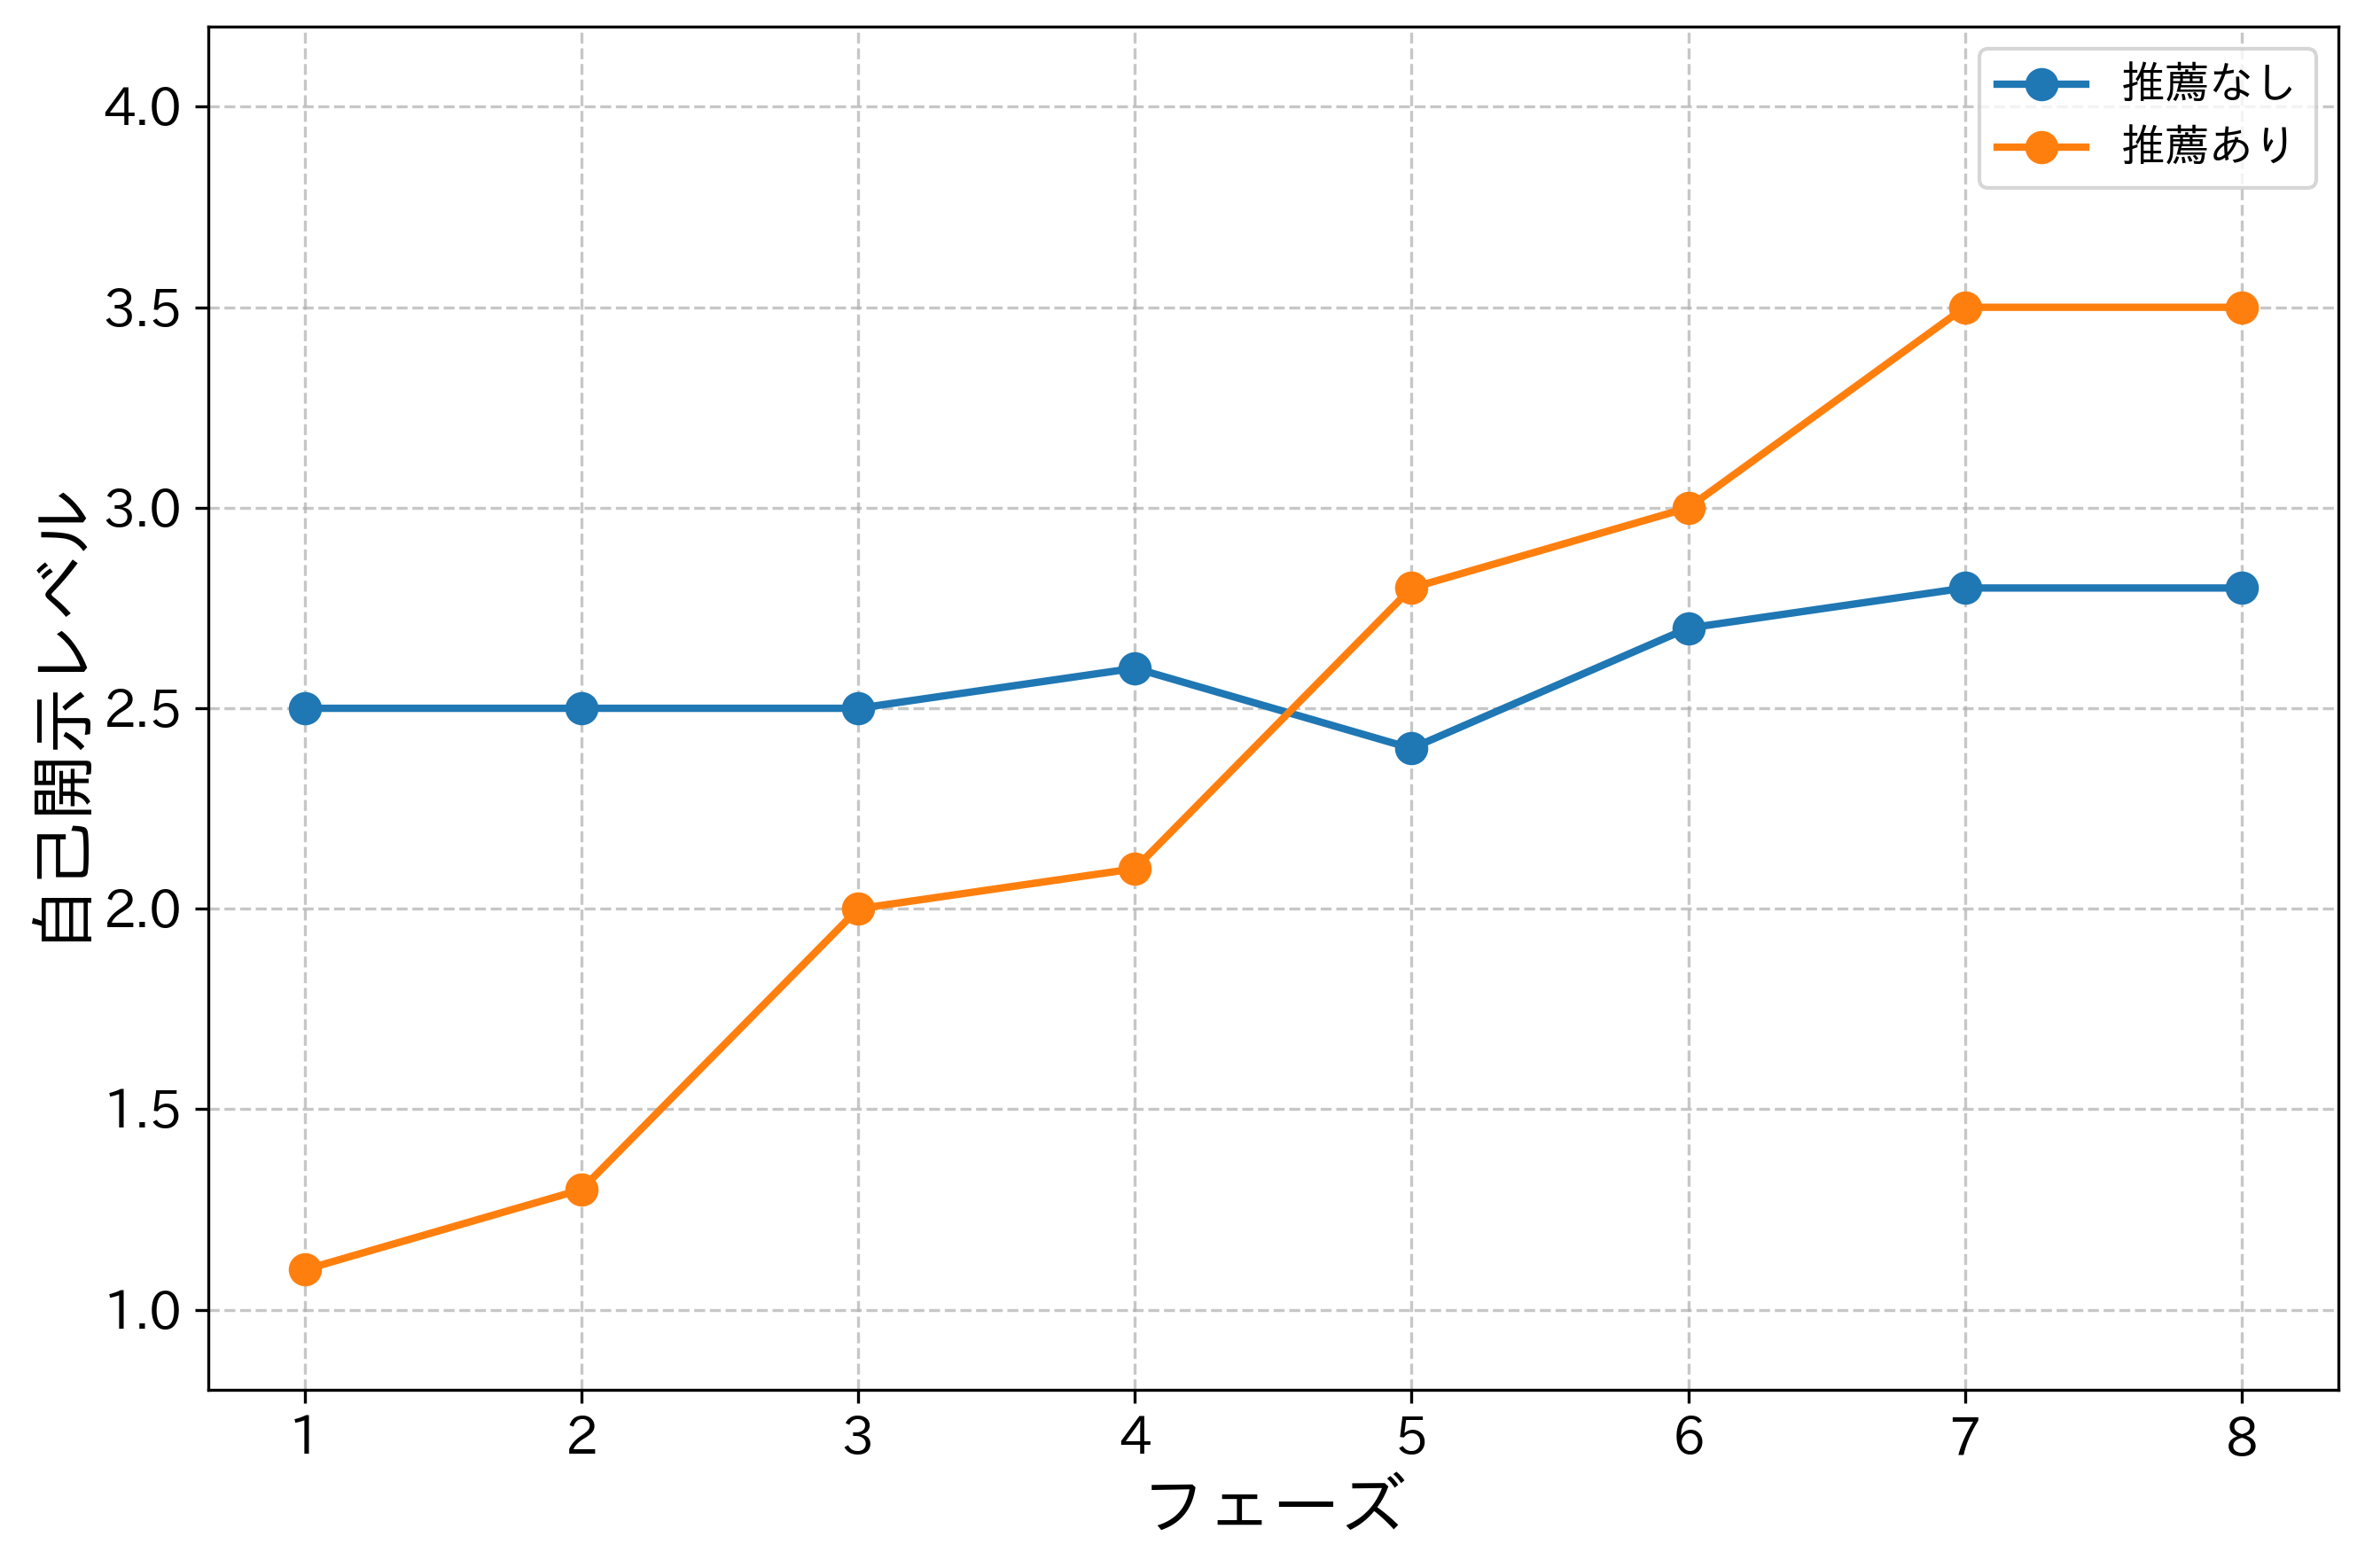
\includegraphics[width=0.9\linewidth]{image/自己開示レベル推移.png}
    \caption{自己開示レベルの推移}
    \label{fig:自己開示レベルの推移}
\end{figure}

実験中のアンケート結果の時系列変化を図\ref{fig:Q5}, 図\ref{fig:Q6}に示す．EQ5（聴いた曲について楽しく話ができた）に関しては，フェーズ5, 6で一時的にスコア4を下回る傾向が見られたものの，最終フェーズ（7, 8）ではレベル3, 4の深い自己開示が行われた状況下でも高い受容度を示した．EQ6（思いや経験が理解できた）の結果からも，推薦あり群は推薦なし群と顕著な差異を示すことなく，特にフェーズ1〜4と7〜8において近似した値を示した．これは，段階的に自己開示を促し深いレベルに到達した場合でも，推薦をしていない群の自己開示と同等の受容度を維持できることを示唆している．具体例として，ユーザーJやKは自己開示レベル4まで到達しながらも，実験開始時からの高い受容度を維持し続けた．

推薦あり群が後半フェーズ（5〜8）で深い自己開示を促されているにも関わらず，推薦なし群と同等の高い受容度を維持していることが確認された．

\begin{figure}[H]
    \centering
    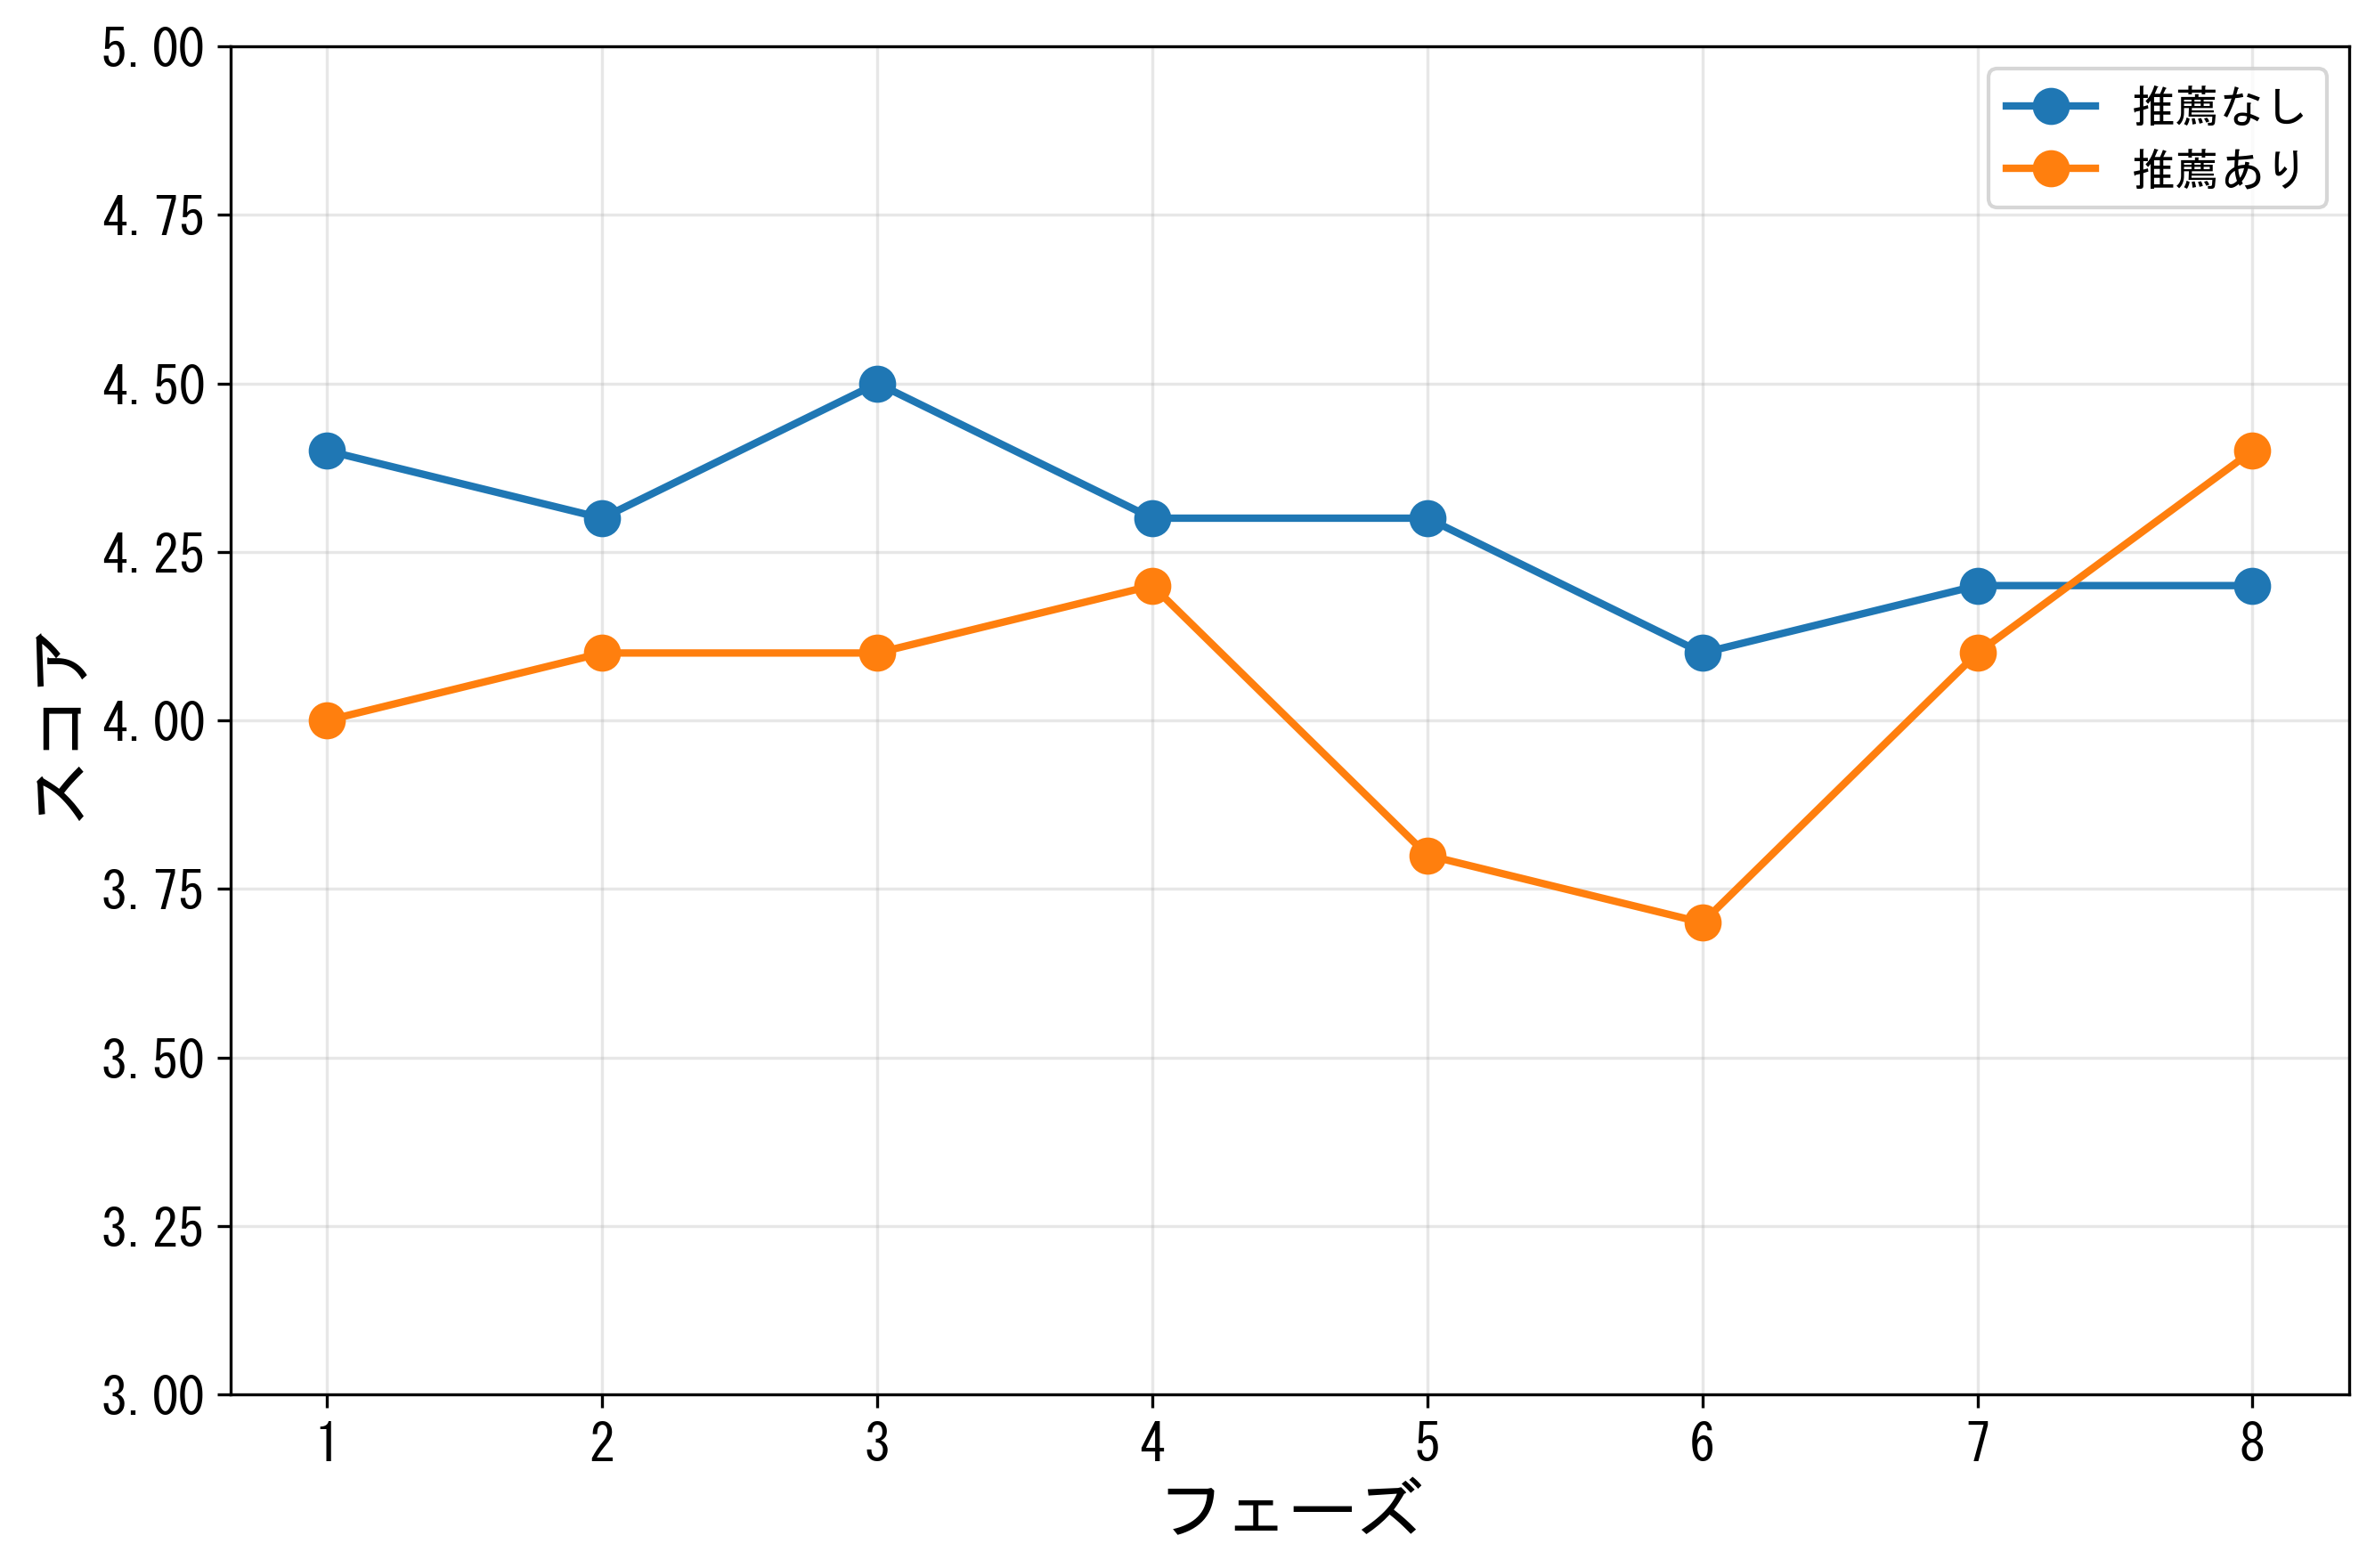
\includegraphics[width=0.9\linewidth]{image/Q5の平均推移.png}
    \caption{EQ5: 聴いた曲について楽しく話ができた}
    \label{fig:Q5}
\end{figure}

\begin{figure}[H]
    \centering
    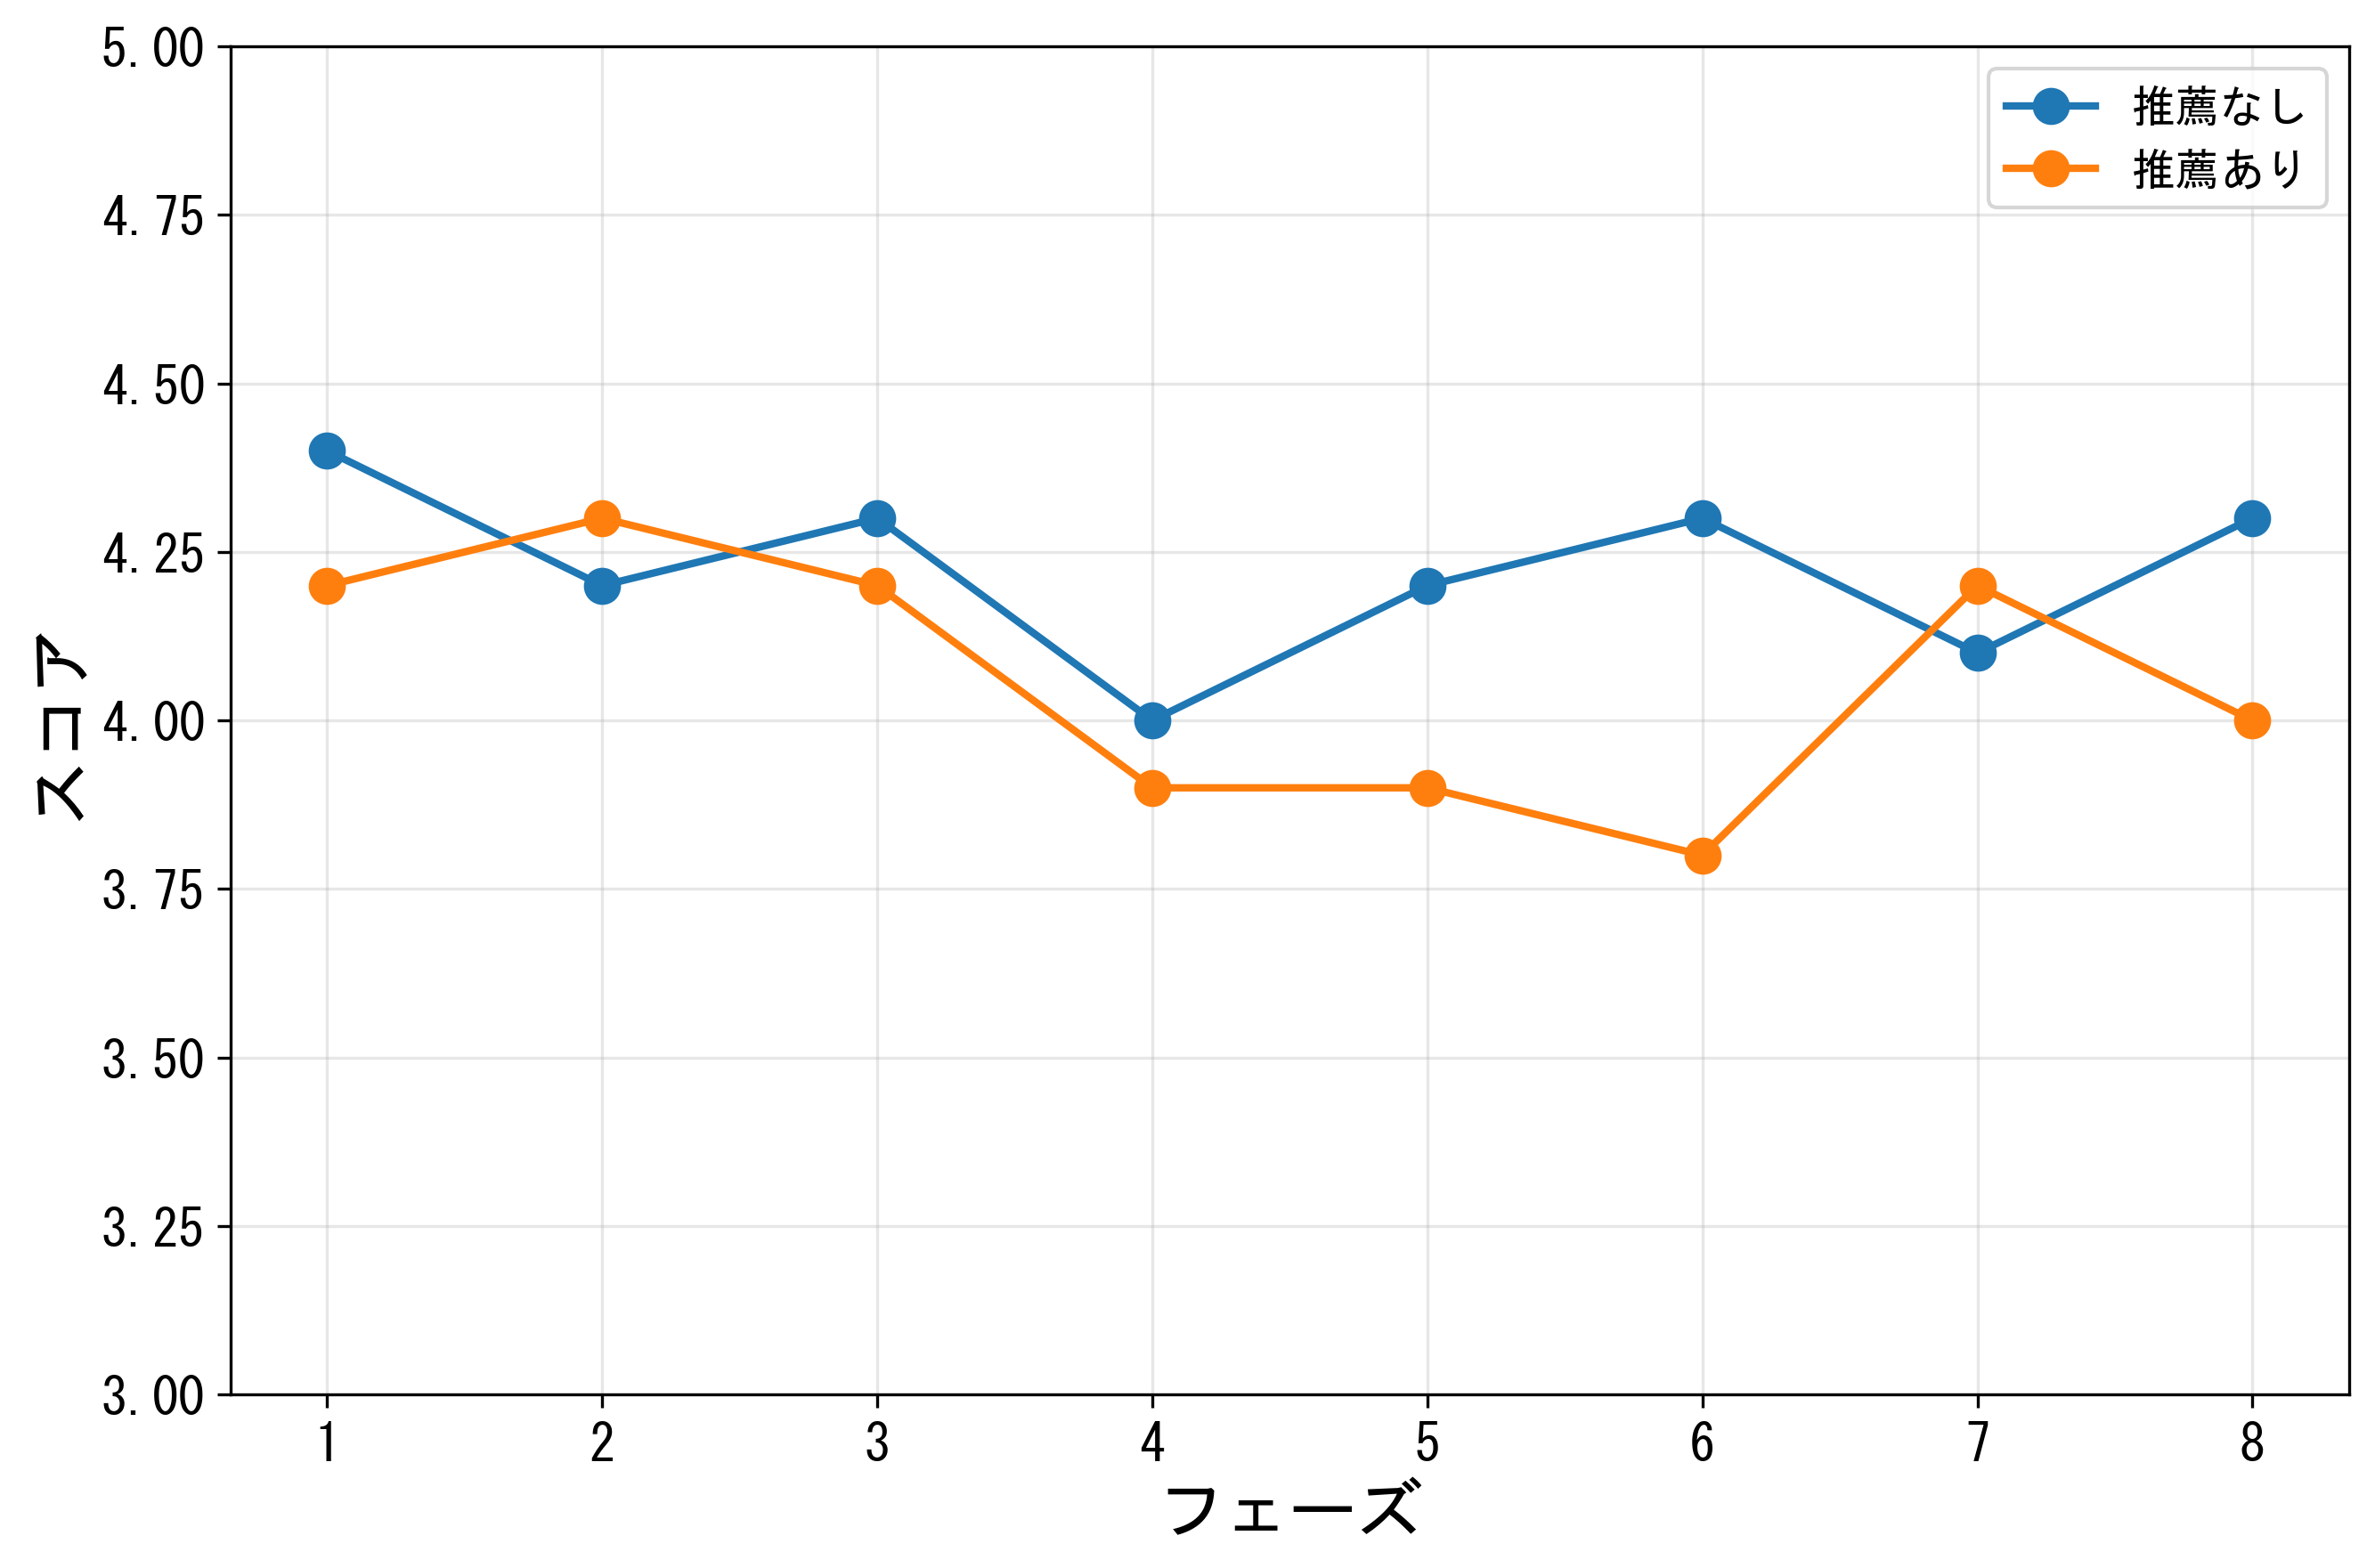
\includegraphics[width=0.9\linewidth]{image/Q6の平均推移.png}
    \caption{Q6: 相手の曲に関する思いや経験が理解できた}
    \label{fig:Q6}
\end{figure}

フェーズを独立変数，各評価項目のスコアを従属変数として単回帰分析を行った結果を表\ref{回帰係数}に示す．いずれの項目においても統計的有意差（p < 0.05）は認められなかったものの，群間で異なる傾向が観察された．推薦あり群ではEQ1（流した曲について楽しく話ができた），EQ2（自分の思いが理解してもらえた）において前半から後半にかけて正の回帰係数を示し，特にEQ5（聴いた曲について楽しく話ができた）の会話の楽しさにおいて向上傾向（β = 0.014）が確認された．これは段階的な自己開示が会話の質的向上と自己開示の受容認知の促進に寄与した可能性を示唆している．対照的に，推薦なし群ではすべての項目で負の回帰係数を示した．初期の受容度は維持されたものの自己開示のレベルが一定に留まったため，会話が表面的なものに留まり，既知の情報で会話が盛り上がってしまったことが原因であると考えられる．ただし，これらの傾向は統計的な裏付けを得るには至らず，より大規模なサンプルでの検証が必要である．

\begin{table}[H]
\caption{群ごとの自己開示の効果分析結果}
\label{回帰係数}
\begin{center}
\begin{tabular}{llcc}
\hline
立場 & 評価項目 & 群 & 回帰係数 β (p値) \\
\hline
\multirow{4}{*}{開示者} & \multirow{2}{*}{EQ1:会話の楽しさ} 
  & 推薦なし & -0.025 (0.488) \\
  & & 推薦あり & 0.080 (0.119) \\
\cline{2-4}
  & \multirow{2}{*}{EQ2:理解された実感} 
  & 推薦なし & -0.037 (0.440) \\
  & & 推薦あり & 0.051 (0.316) \\
\hline
\multirow{4}{*}{被開示者} & \multirow{2}{*}{EQ5:会話の楽しさ} 
  & 推薦なし & -0.037 (0.305) \\
  & & 推薦あり & 0.014 (0.761) \\
\cline{2-4}
  & \multirow{2}{*}{EQ6:相手への理解} 
  & 推薦なし & -0.012 (0.740) \\
  & & 推薦あり & -0.037 (0.493) \\
\hline
\end{tabular}
\end{center}
\end{table}

表\ref{table:群別の自己開示レベルごとの曲数と人数}に，各群における自己開示レベル別の集計結果を示す．この表は，各自己開示レベルについて，選曲された総数（曲数）と，そのレベルの曲を少なくとも1回選曲したユーザーの人数を示している．例えば，推薦なし群ではレベル3の曲が全体で45曲選曲され，9人のユーザーがレベル3の曲を1曲以上選んでいたことを表している．

本仮説の検証における問題として，レベル4の自己開示の出現頻度の低さが挙げられる．推薦なし群において観察されたレベル4の自己開示は全体でわずか6回に留まり，その結果，いきなり深い自己開示をしたときとの比較などを行うことができなかった．しかしながら，この現象自体が，友人関係においても最も深い自己開示が自然には起こりづらいという既存の知見を指示するものとして捉えられる．

\begin{table}[H]
  \centering
  \caption{群別の自己開示レベルごとの曲数と人数}
  \label{群別の自己開示レベルごとの曲数と人数}
  \begin{tabular}{llcccc}
    \hline
    群 & 種別 & レベル1 & レベル2 & レベル3 & レベル4 \\
    \hline
    \multirow{2}{*}{推薦なし} & 曲数[曲] & 9 & 20 & 45 & 6 \\
    & 人数[人] & 3 & 9 & 9 & 4 \\
    \hline
    \multirow{2}{*}{推薦あり} & 曲数[曲] & 17 & 23 & 30 & 10 \\
    & 人数[人] & 9 & 10 & 10 & 6 \\
    \hline
  \end{tabular}
  \label{table:群別の自己開示レベルごとの曲数と人数}
\end{table}



\subsection{仮説2の結果}\label{仮説2の結果}

\ref{研究課題と仮説}節で述べたように，仮説2は「音楽への認知度が低い，または興味度が低い場合でも，自己開示の受容度は大きく低下しない」である．
これを検証するため，EQ3（曲を知っているか）とEQ4（曲に興味を持てたか）の回答値の違いが，受容度（EQ5, EQ6）にどの程度影響を与えるか分析を行った．具体的には，EQ3（曲を知っているか）については知っている場合（1）の受容度（EQ5, EQ6）から知らない場合（0）の受容度（EQ5, EQ6）を引いた値を，EQ4（曲に興味を持てたか）については高い興味度（4-5）の受容度（EQ5, EQ6）から低い興味度（1-3）の受容度（EQ5, EQ6）を引いた値を，各ユーザーごとに算出した．表\ref{tab:differences}に各質問項目における差分の平均値と標準偏差を示す．

\begin{table}[H]
  \centering
  \begin{tabular}{ccc}
    \hline
    項目 & 平均 & 標準偏差 \\
    \hline
    各ユーザーごとのEQ3の値によるEQ5の差分 & 0.24 & 0.64 \\
    各ユーザーごとのEQ3の値によるEQ6の差分 & 0.00 & 0.72 \\
    各ユーザーごとのEQ4の値によるEQ5の差分 & 0.51 & 0.88 \\
    各ユーザーごとのEQ4の値によるEQ6の差分 & 0.23 & 0.61 \\
    \hline
  \end{tabular}
  \caption{各質問項目における差分の平均値と標準偏差}
  \label{tab:differences}
\end{table}

図\ref{EQ3比較差分のやつ}に示すように，認知度（EQ3）の影響については19名のユーザーデータを分析することができた．一方，図\ref{EQ4比較差分のやつ}に示すように，興味度（EQ4）については，興味度のスコアが1～3と，4～5が混在するユーザーは10名のみであった．

\begin{figure}[H]
    \centering
    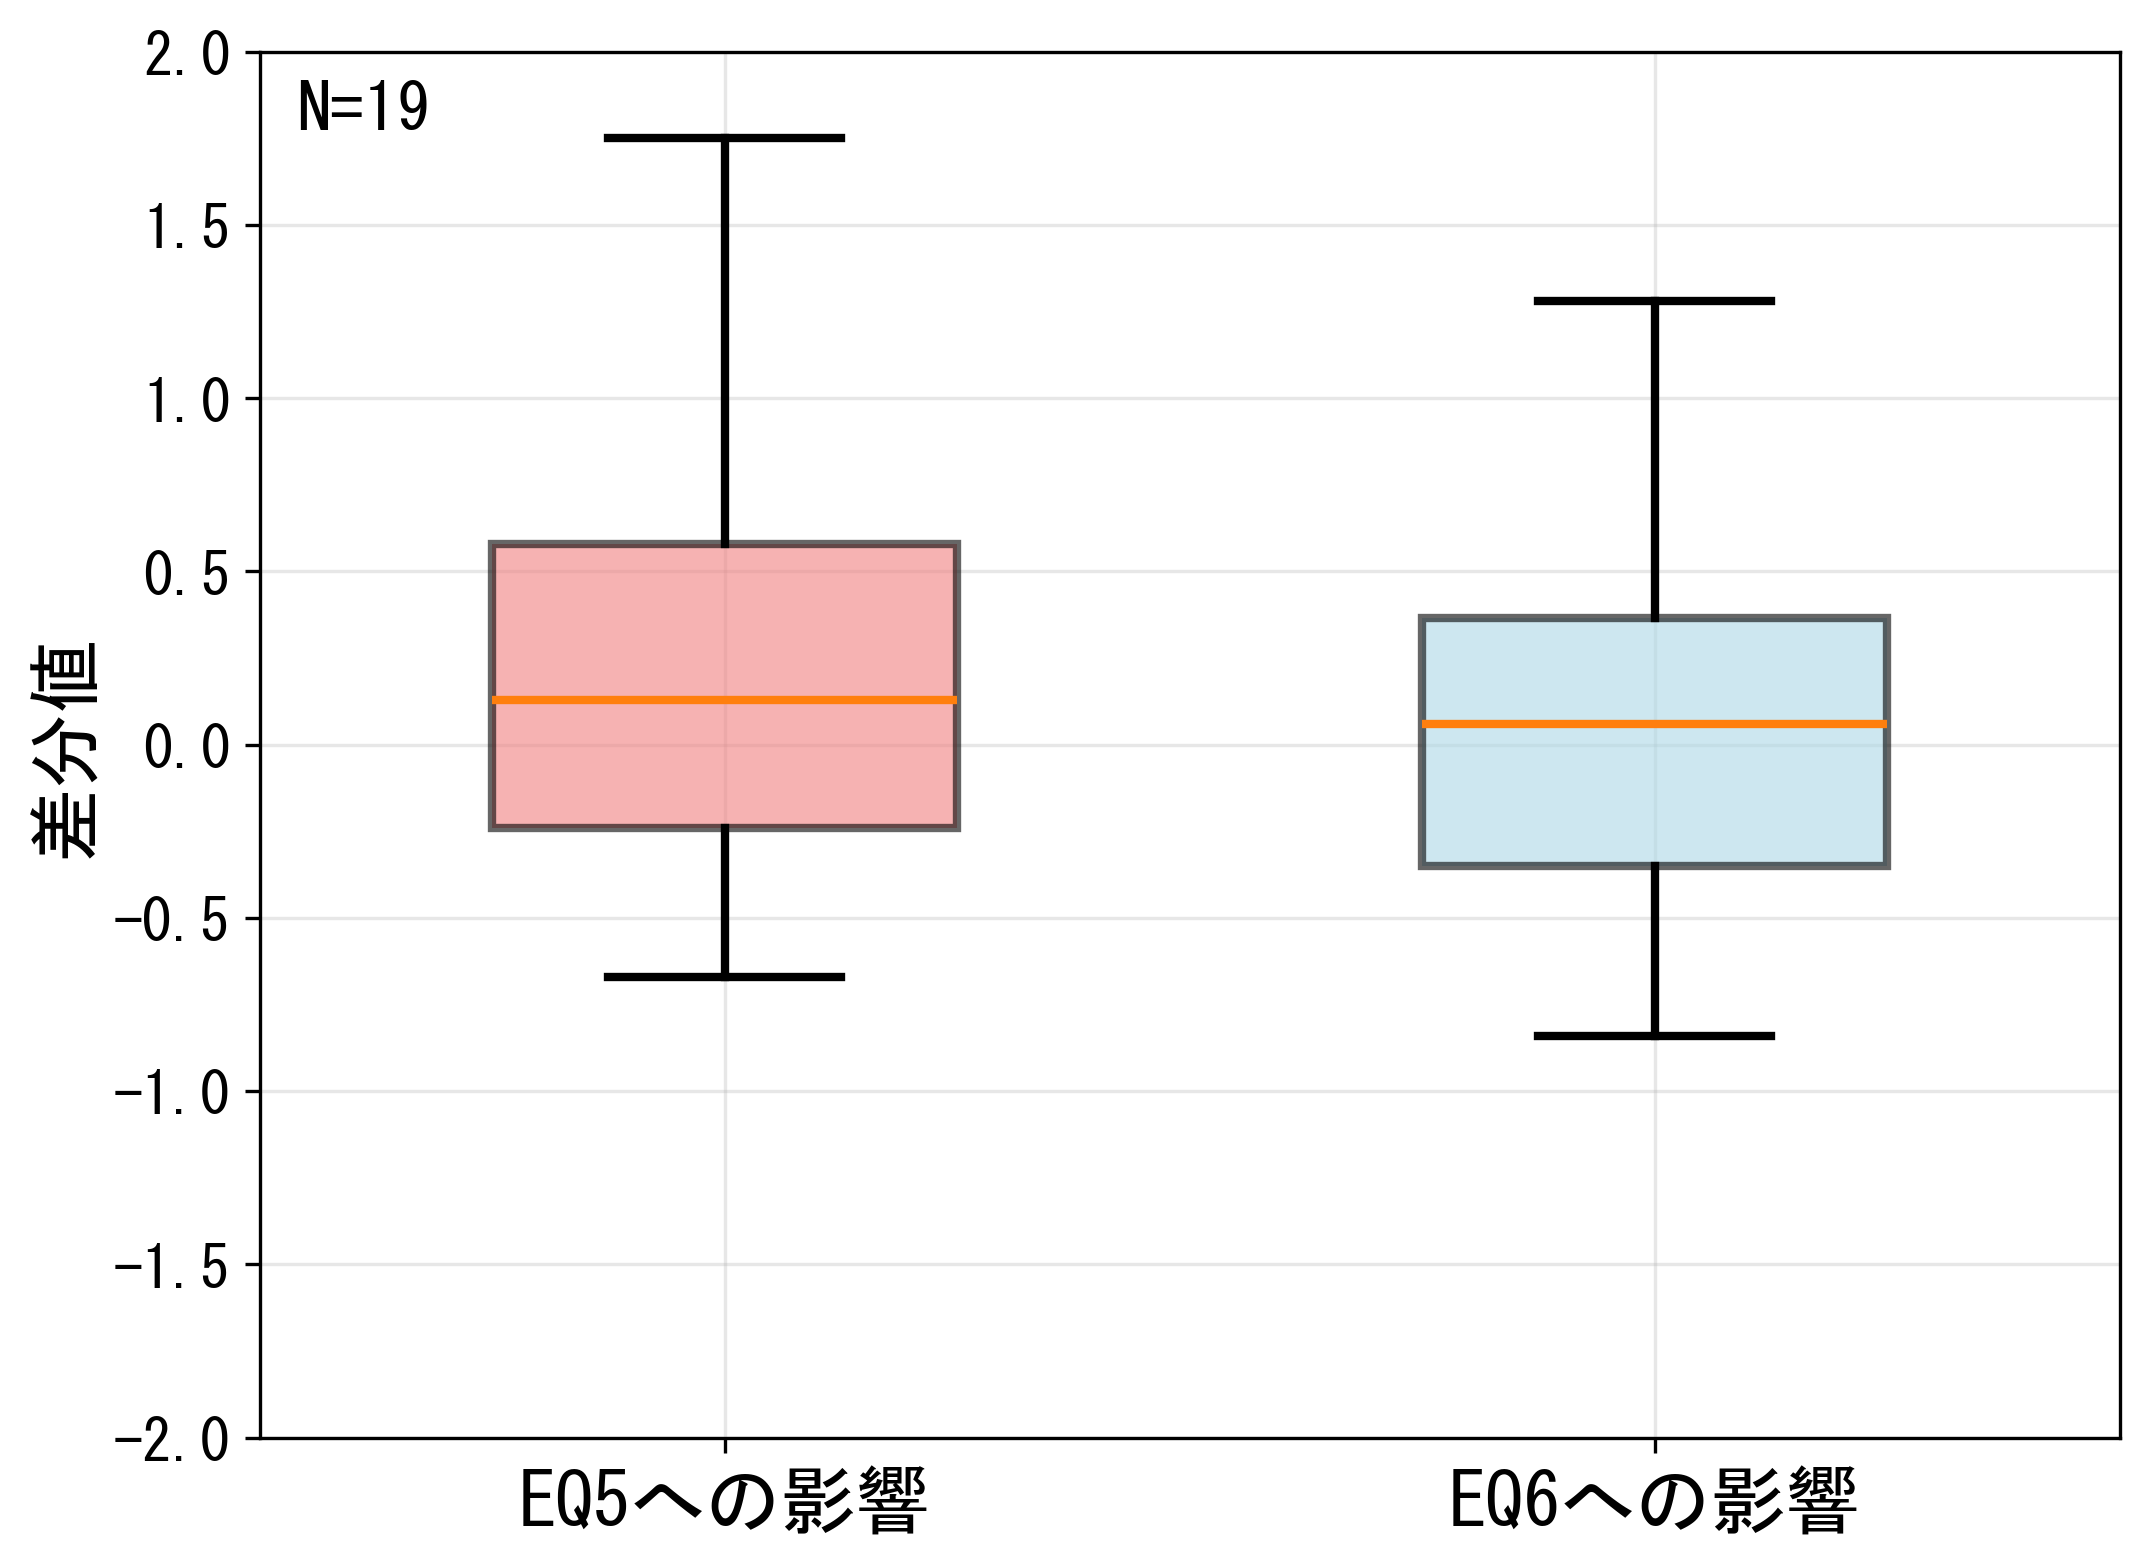
\includegraphics[width=0.75\linewidth]{image/EQ3比較差分のやつ.png}
    \caption{曲の認知度（EQ3）による受容度の差異}
    \label{EQ3比較差分のやつ}
\end{figure}

\begin{figure}[H]
    \centering
    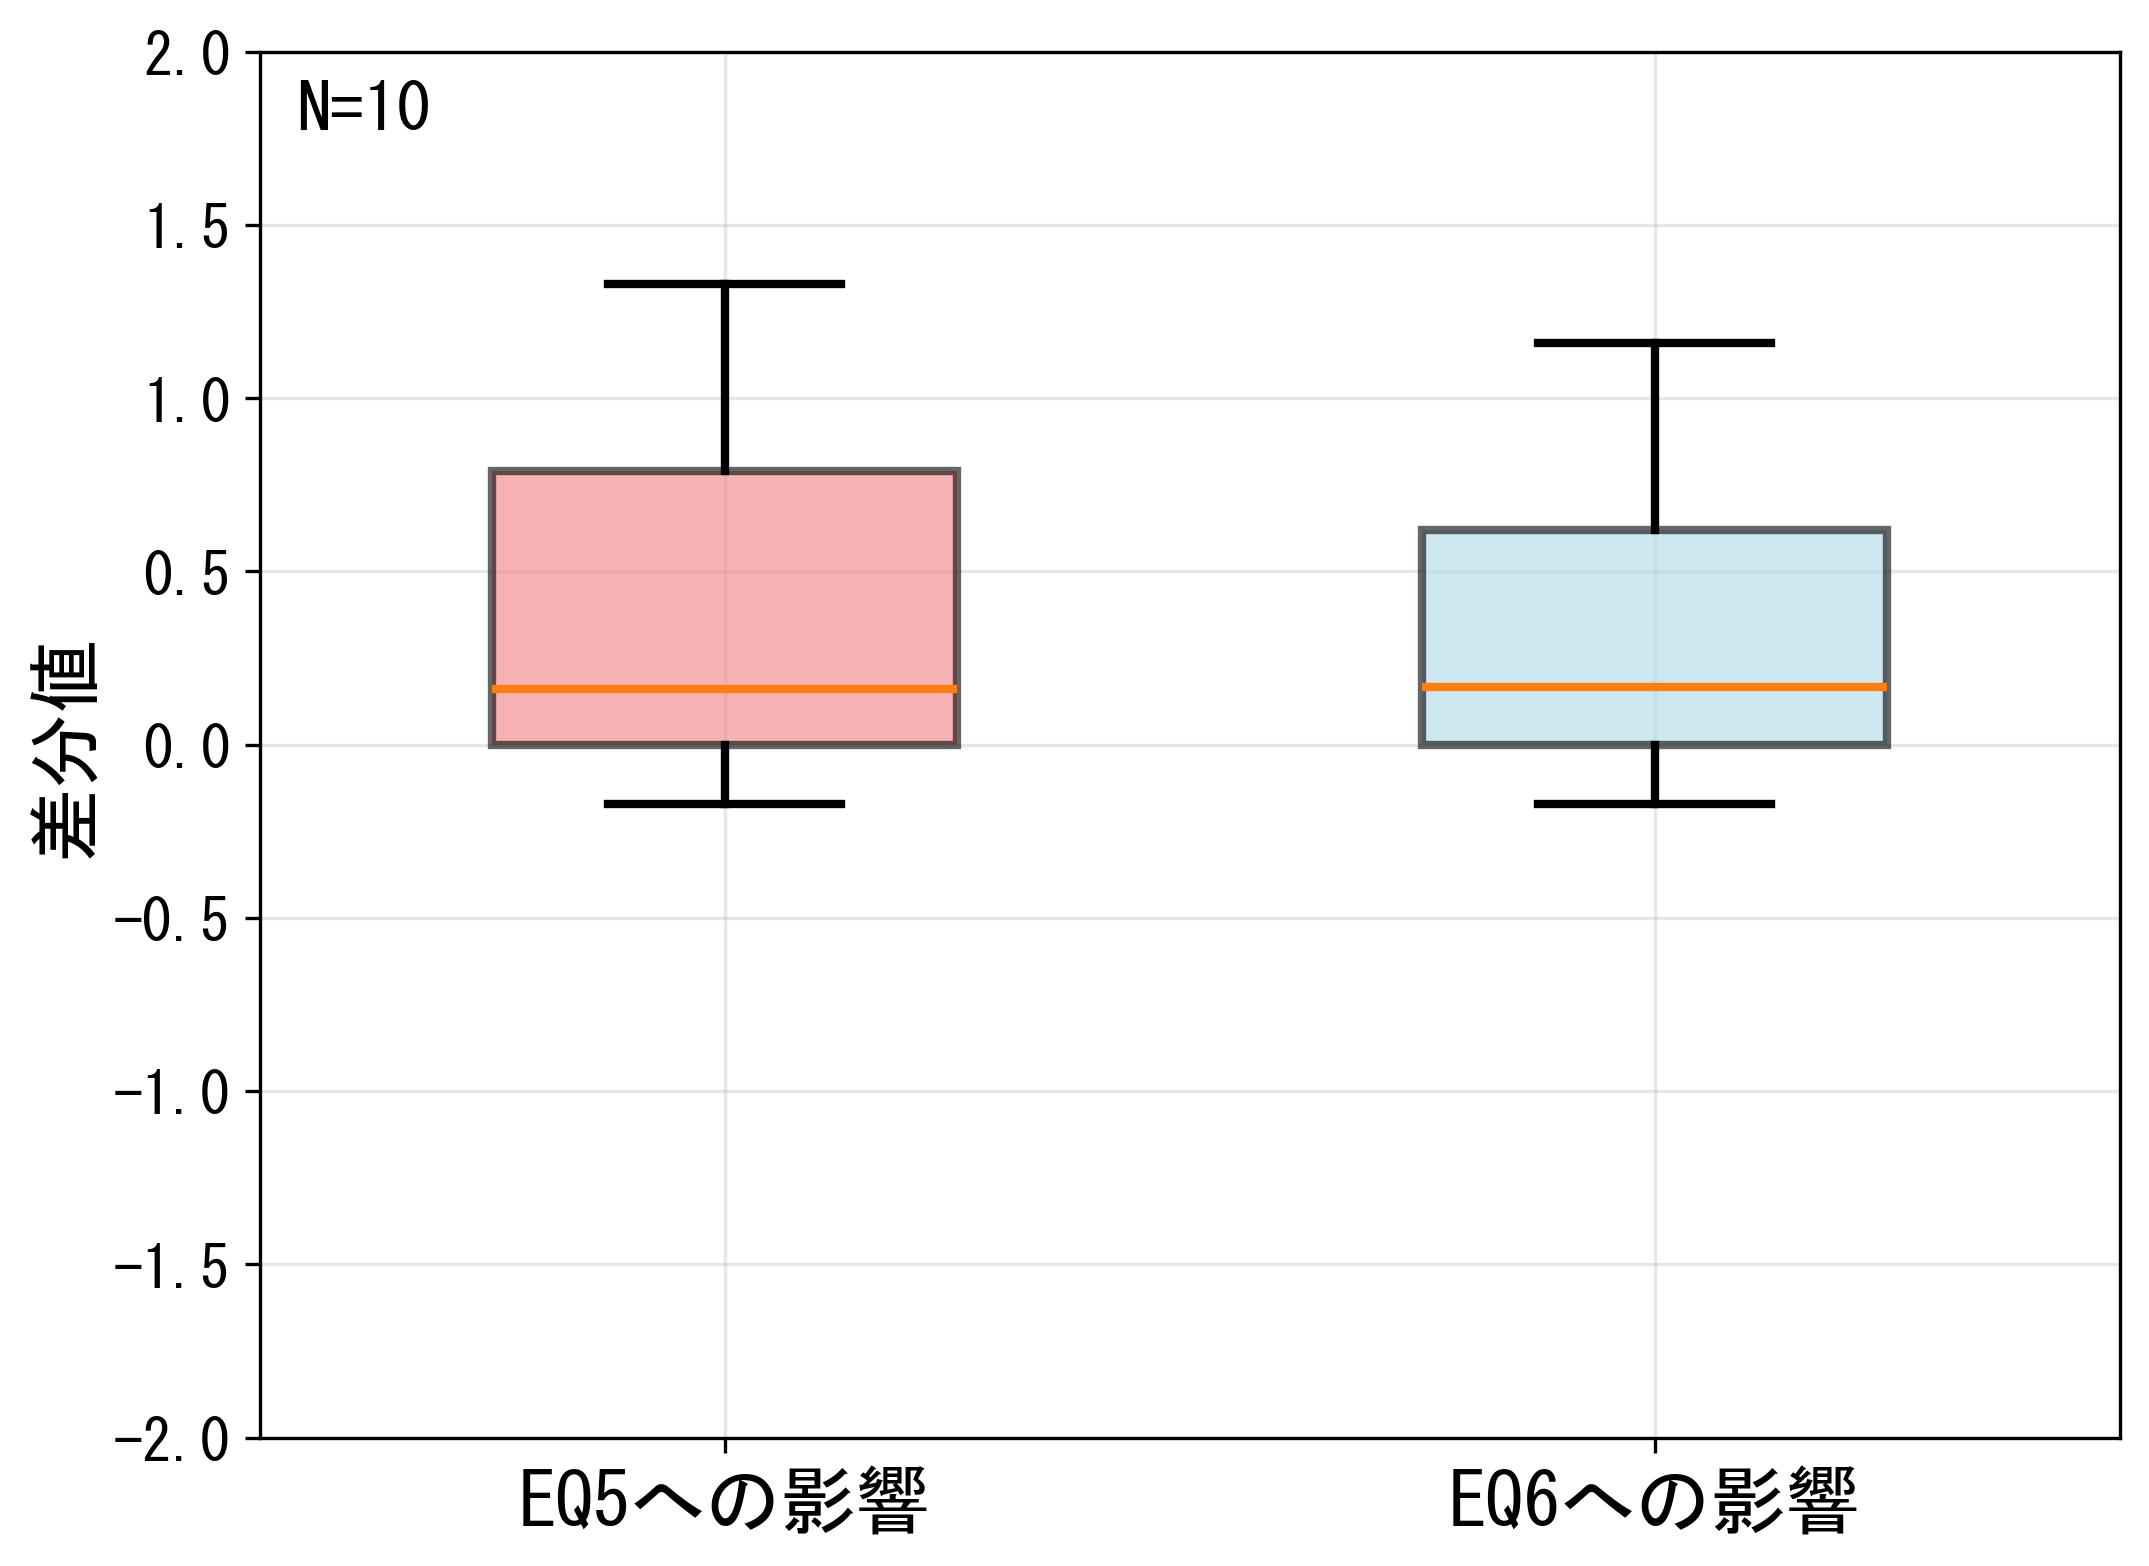
\includegraphics[width=0.75\linewidth]{image/EQ4比較差分のやつ.png}
    \caption{曲の興味度（EQ4）による受容度の差異}
    \label{EQ4比較差分のやつ}
\end{figure}

認知度（EQ3）の影響について，表\ref{tab:differences}に示すように，EQ5（聴いた曲について楽しく話ができた）とEQ6（思いや経験が理解できた）への差分平均値はそれぞれ0.24（標準偏差0.64）と0.00（標準偏差0.72）となった．図\ref{EQ3比較差分のやつ}から分かるように，EQ5（聴いた曲について楽しく話ができた）への影響はプラスの傾向を示すものの，データの分布は比較的狭い範囲に収まっている．EQ6（思いや経験が理解できた）への影響はさらに顕著で，中央値がほぼ0に近く，データのばらつきも小さいことから，曲の認知度が相手の思いや経験の理解にほとんど影響を与えていないことを示している．

次に，興味度（EQ4）の影響については，10名のデータを分析した結果，EQ5（聴いた曲について楽しく話ができた）とEQ6（思いや経験が理解できた）への差分平均値がそれぞれ0.51（標準偏差0.88）と0.23（標準偏差0.61）となった．図\ref{EQ4比較差分のやつ}から分かるように，両方の指標において極端な負の値は見られず，中央値も近い値を示している．
% 特にEQ5への影響については，データの大部分が正の値を示しており，興味度が高い場合の方が受容度が高い傾向があることが示唆された．
ただし，EQ5（聴いた曲について楽しく話ができた）については標準偏差が大きいことから，データのばらつきが大きく，この傾向は個人差が大きいことが確認された．つまり，興味度の高低が受容度に与える影響は一概に判断できないと考えられる．

興味度と認知度の両方において，値にばらつきは見られるものの四分位範囲は比較的小さく，極端な正負の値も少ないことから，多くのユーザーで安定した結果が得られたと言える．つまり，相手の曲を知らない，あるいは強い興味を持っていない場合であったとしても，自己開示に対する受容度は大きく低下しないことが示された．このことは，音楽への興味度や知識が自己開示の受容に与える影響が限定的であることを示唆している．以上の分析結果から，仮説2「被開示者の音楽への興味度に関わらず，高い受容度を示す」については支持されたと考えられる．



\subsection{仮説3の結果}\label{仮説3の結果}

\ref{研究課題と仮説}節で述べた仮説3「セッションを終えた2者は，段階的に自己開示を促していない方に比べて相手に対する受容性が向上する」について検証を行った．
実験後のアンケートを平均値にした図\ref{fig:事後アンケート}では，全項目について推薦あり群より推薦なし群の方が満足度が高く，特にPQ6（実験前より相手の音楽の好みについて理解できた）は推薦なし群の方が1ポイントほど高いことが分かる．これは，セッション内での自己開示レベルの高い曲への受容性は向上していたものの，序盤は自己開示レベルの低い曲しか選曲できなかったことから，全体を通して深い自己開示があまりできず，相互理解の促進に繋がらなかったのではないかと考えられる．

推薦なし群と推薦あり群の間で評価値の分布に有意な差があるかを検討するために，Mann-WhitneyのU検定を行った．すると，PQ6の項目においてのみ有意な差（U = 83.000, p = 0.006, r = .609）が見られた．
しかし，PQ5（U = 53.500, p = 0.805, r = .055）およびPQ7（U = 61.500, p = 0.335, r = .216）では有意な差は見られなかった．両項目において，両群ともに高い評価値（4ポイント以上）を示しており，これは推薦システムの有無に関わらず，音楽を介した対話が相互理解と音楽を通じたコミュニケーションの意欲を促進する可能性を示唆している．

\begin{figure}[H]
    \centering
    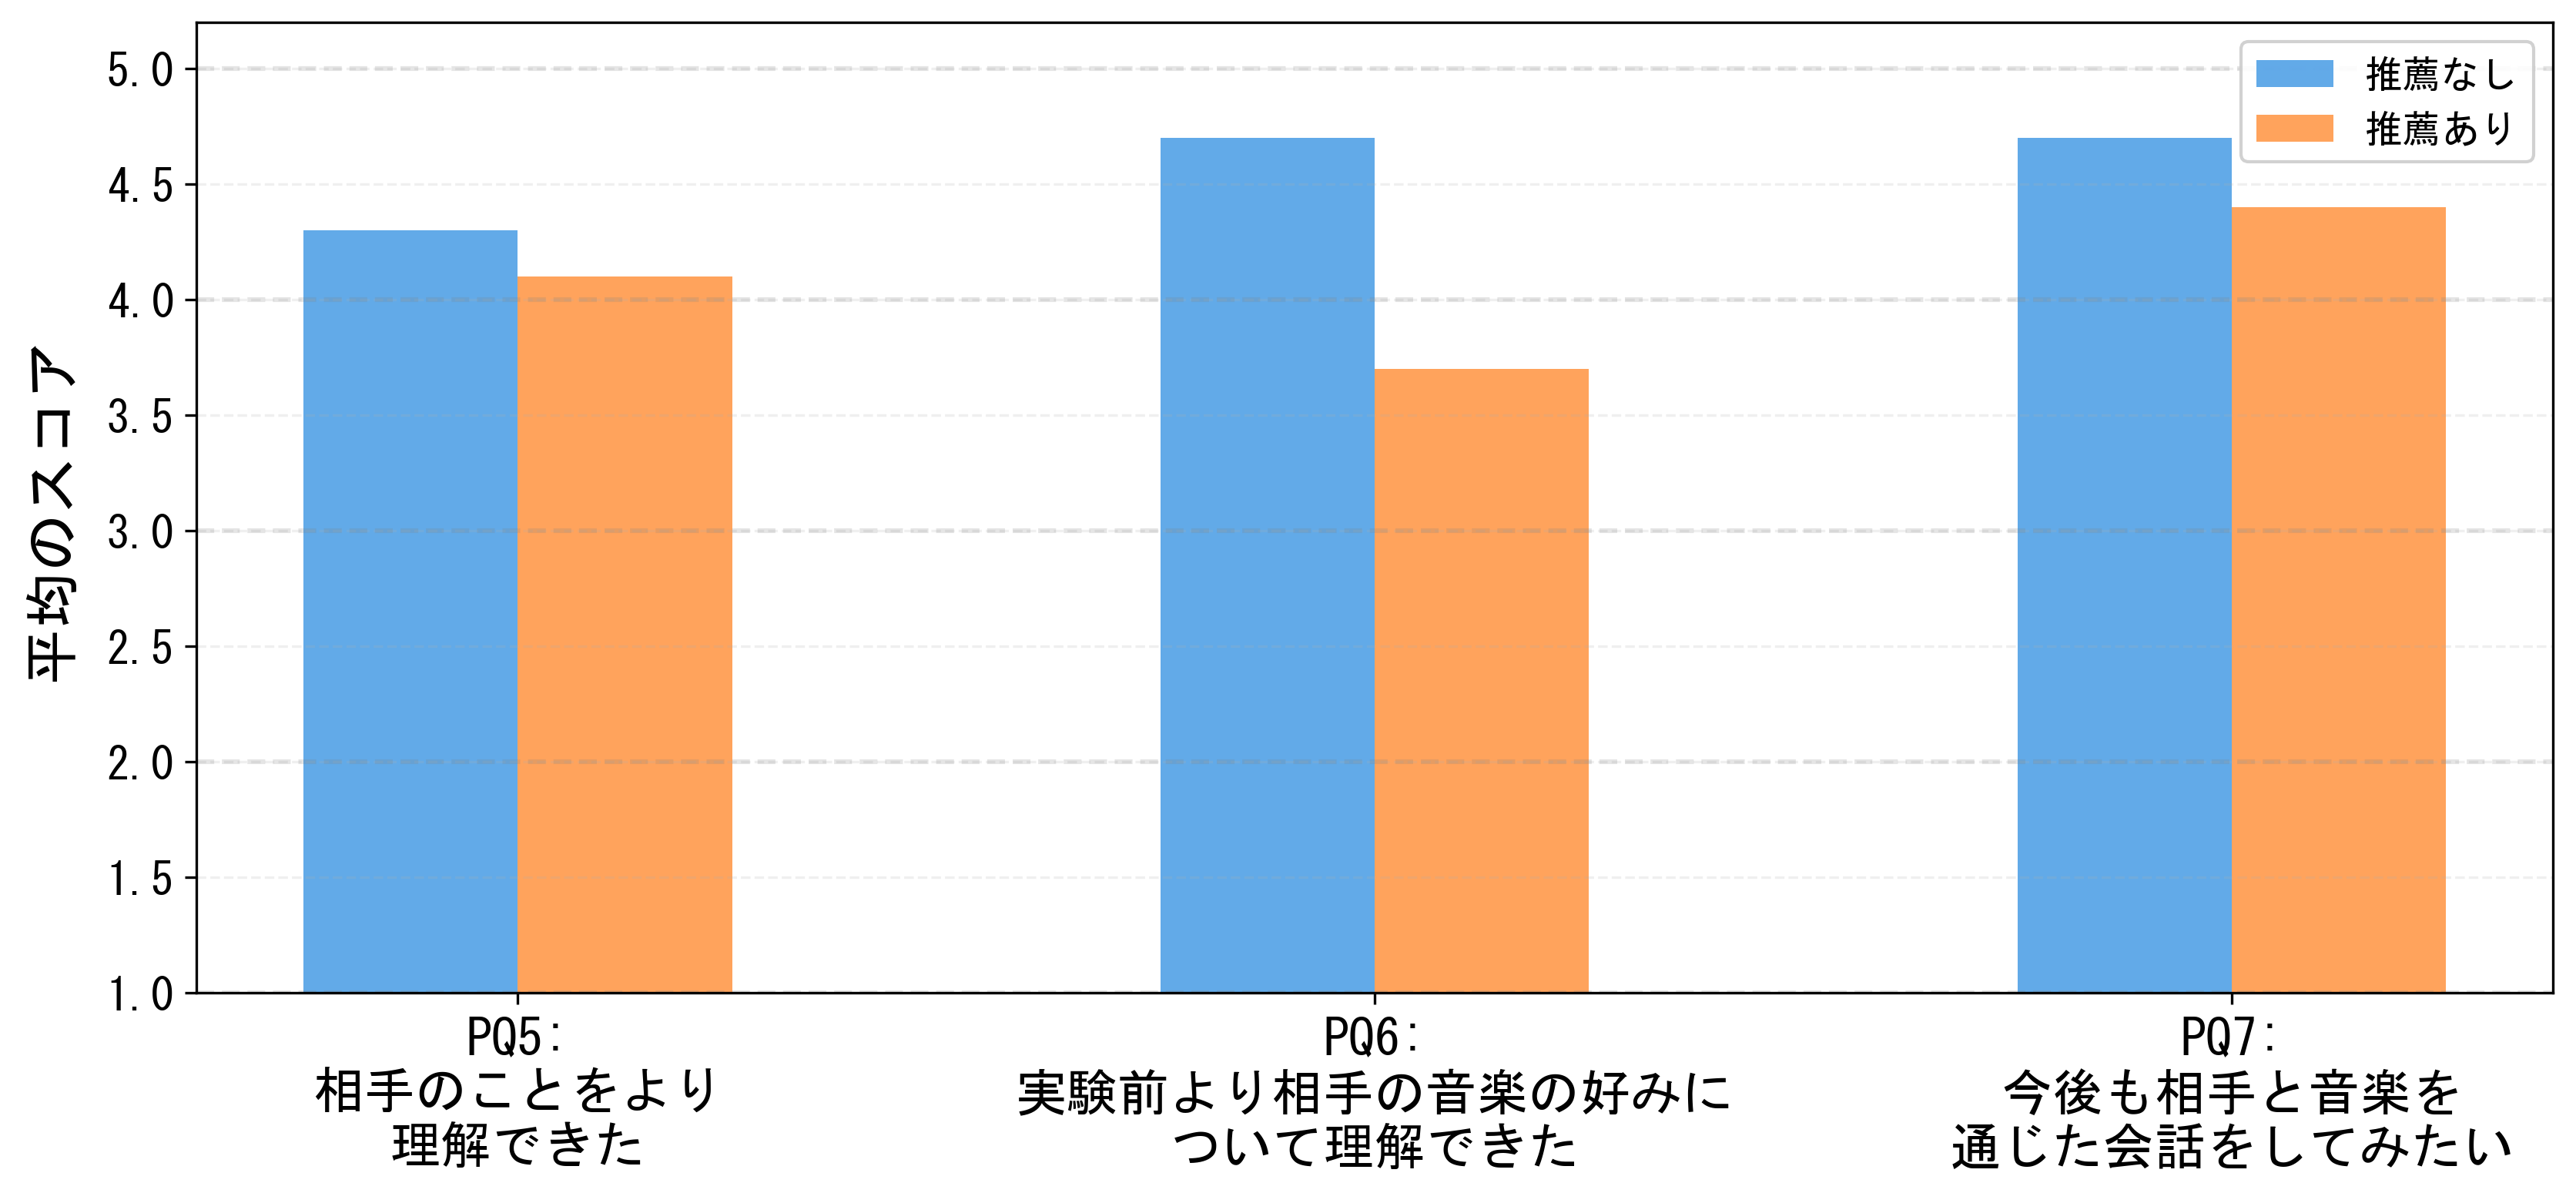
\includegraphics[width=1\linewidth]{image/実験後の受容質問3つ.png}
    \caption{実験後アンケート結果の比較}
    \label{fig:事後アンケート}
\end{figure}


各被験者の実験後アンケート結果を，表\ref{fig:実験後アンケート表}に示す．多くの被験者がPQ5（相手のことをより理解できた），PQ6（実験前より相手の音楽の好みについて理解できた），PQ7（今後も相手と音楽を通じた会話をしてみたい）の3項目について4点または5点の高評価を示した中で，特徴的な回答が見られた．

推薦あり群のアンケートの平均値が下がった理由として，ペア3の結果が挙げられる．
ペア3は他のペアと比較して顕著に低い評価が観察され，特に被験者Fの回答（PQ5：3点，PQ6：1点，PQ7：3点）は全被験者の中で特に低い値を示した．被験者FのPQ4（自分の内面についてよく話すことができた）で1点を示しているように，ヒアリングから，音楽についてうまく話せないことに苛立ちを覚えて，自己嫌悪し，空気を悪くしてしまったことが明らかになった．一方で，システムによる推薦に対しての不満はなく，被験者Eからは「どの曲も話した過ぎて何を選ぶか悩んだ」という報告があり，段階的な推薦は悪影響を及ぼしていないことが確認された．

対照的に，推薦あり群のペア10については，普段からよく音楽の話をしているが，様々なジャンルについて触れて話ができたり，相手のことを深く知ることができたと答えていた．システムが提示した4つの選択肢には，いずれも対話の題材として魅力的な楽曲が含まれており，選曲の意思決定にポジティブな迷いが生じたことが報告された．このことは，システムによる楽曲推薦が有効な選択肢を提供できていたことを示唆している．

さらに，ヒアリングの結果，推薦なし群からは「相手の音楽の趣味が思ったより異なることが分かった」「相手の好きな音楽についてより深く理解できた」といった音楽嗜好の表面的な理解に関する言及が多く見られた．一方で，推薦あり群からは「相手のことを深く知ることができた」「なぜ曲を好きになったか，曲に対する熱意を知れた」など，音楽を通じた個人的な思い出や背景についての言及がされていた．この結果は，段階的な音楽推薦システムが，単に音楽の好みを共有するだけでなく，被験者間のより深い相互理解の形成に寄与する可能性を示している．


\begin{figure}[H]
    \centering
    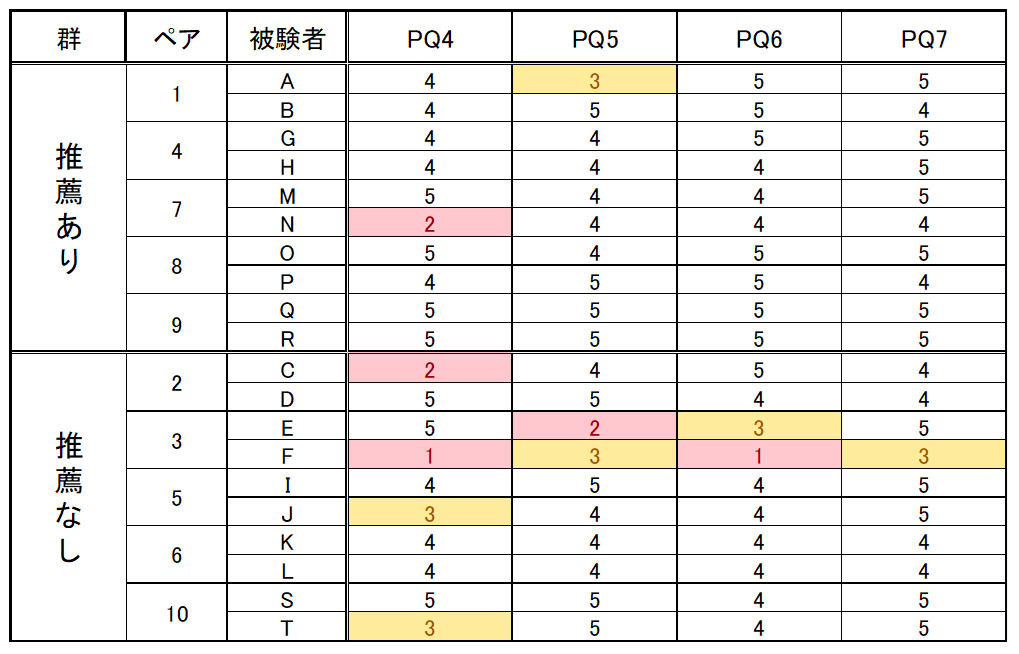
\includegraphics[width=0.9\linewidth]{image/実験後アンケート表2.png}
    \caption{被験者ごとの実験後アンケート（PQ4～PQ7）}
    \label{fig:実験後アンケート表}
\end{figure}


\begin{comment}
    実験序盤から終盤での差異を見るため，EQ5, EQ6について，後半フェーズ（7～8）の平均値から前半フェーズ（1～2）の平均値を減算し，その変化量を算出した．その結果を図\ref{fig:EQ5-最初to最後の変化量}, 図\ref{fig:EQ6-最初to最後の変化量}に示す．
    
    EQ5については，推薦あり群では平均0.20ポイントの向上が見られたが，推薦なし群では平均-0.15ポイントの低下が確認された．また，標準偏差は推薦あり群（0.632）の方が推薦なし群（0.973）より小さく，段階に推薦をすることによって，より安定した効果が得られたことが示唆された．
    一方，EQ6については，推薦なし群（標準偏差0.775）および推薦あり群（標準偏差0.626）の両群において，平均値では若干の低下傾向が観察された．しかし，分布の形状に着目すると，推薦あり群ではデータの上部が正の値まで広く分布しているのに対し，推薦なし群では上方への広がりが小さかった．この分布の特徴は，段階的推薦を受けた推薦あり群において，一部のペアでは相手への理解が深まる可能性があることを示唆している．また，推薦あり群では，全体としては若干の低下傾向を示しているものの，データの上部が正の方向に広く分布しており，個人差はあるものの相手理解の促進に対して良い効果が得られる可能性が示唆された．
    
    \begin{figure}[H]
        \centering
        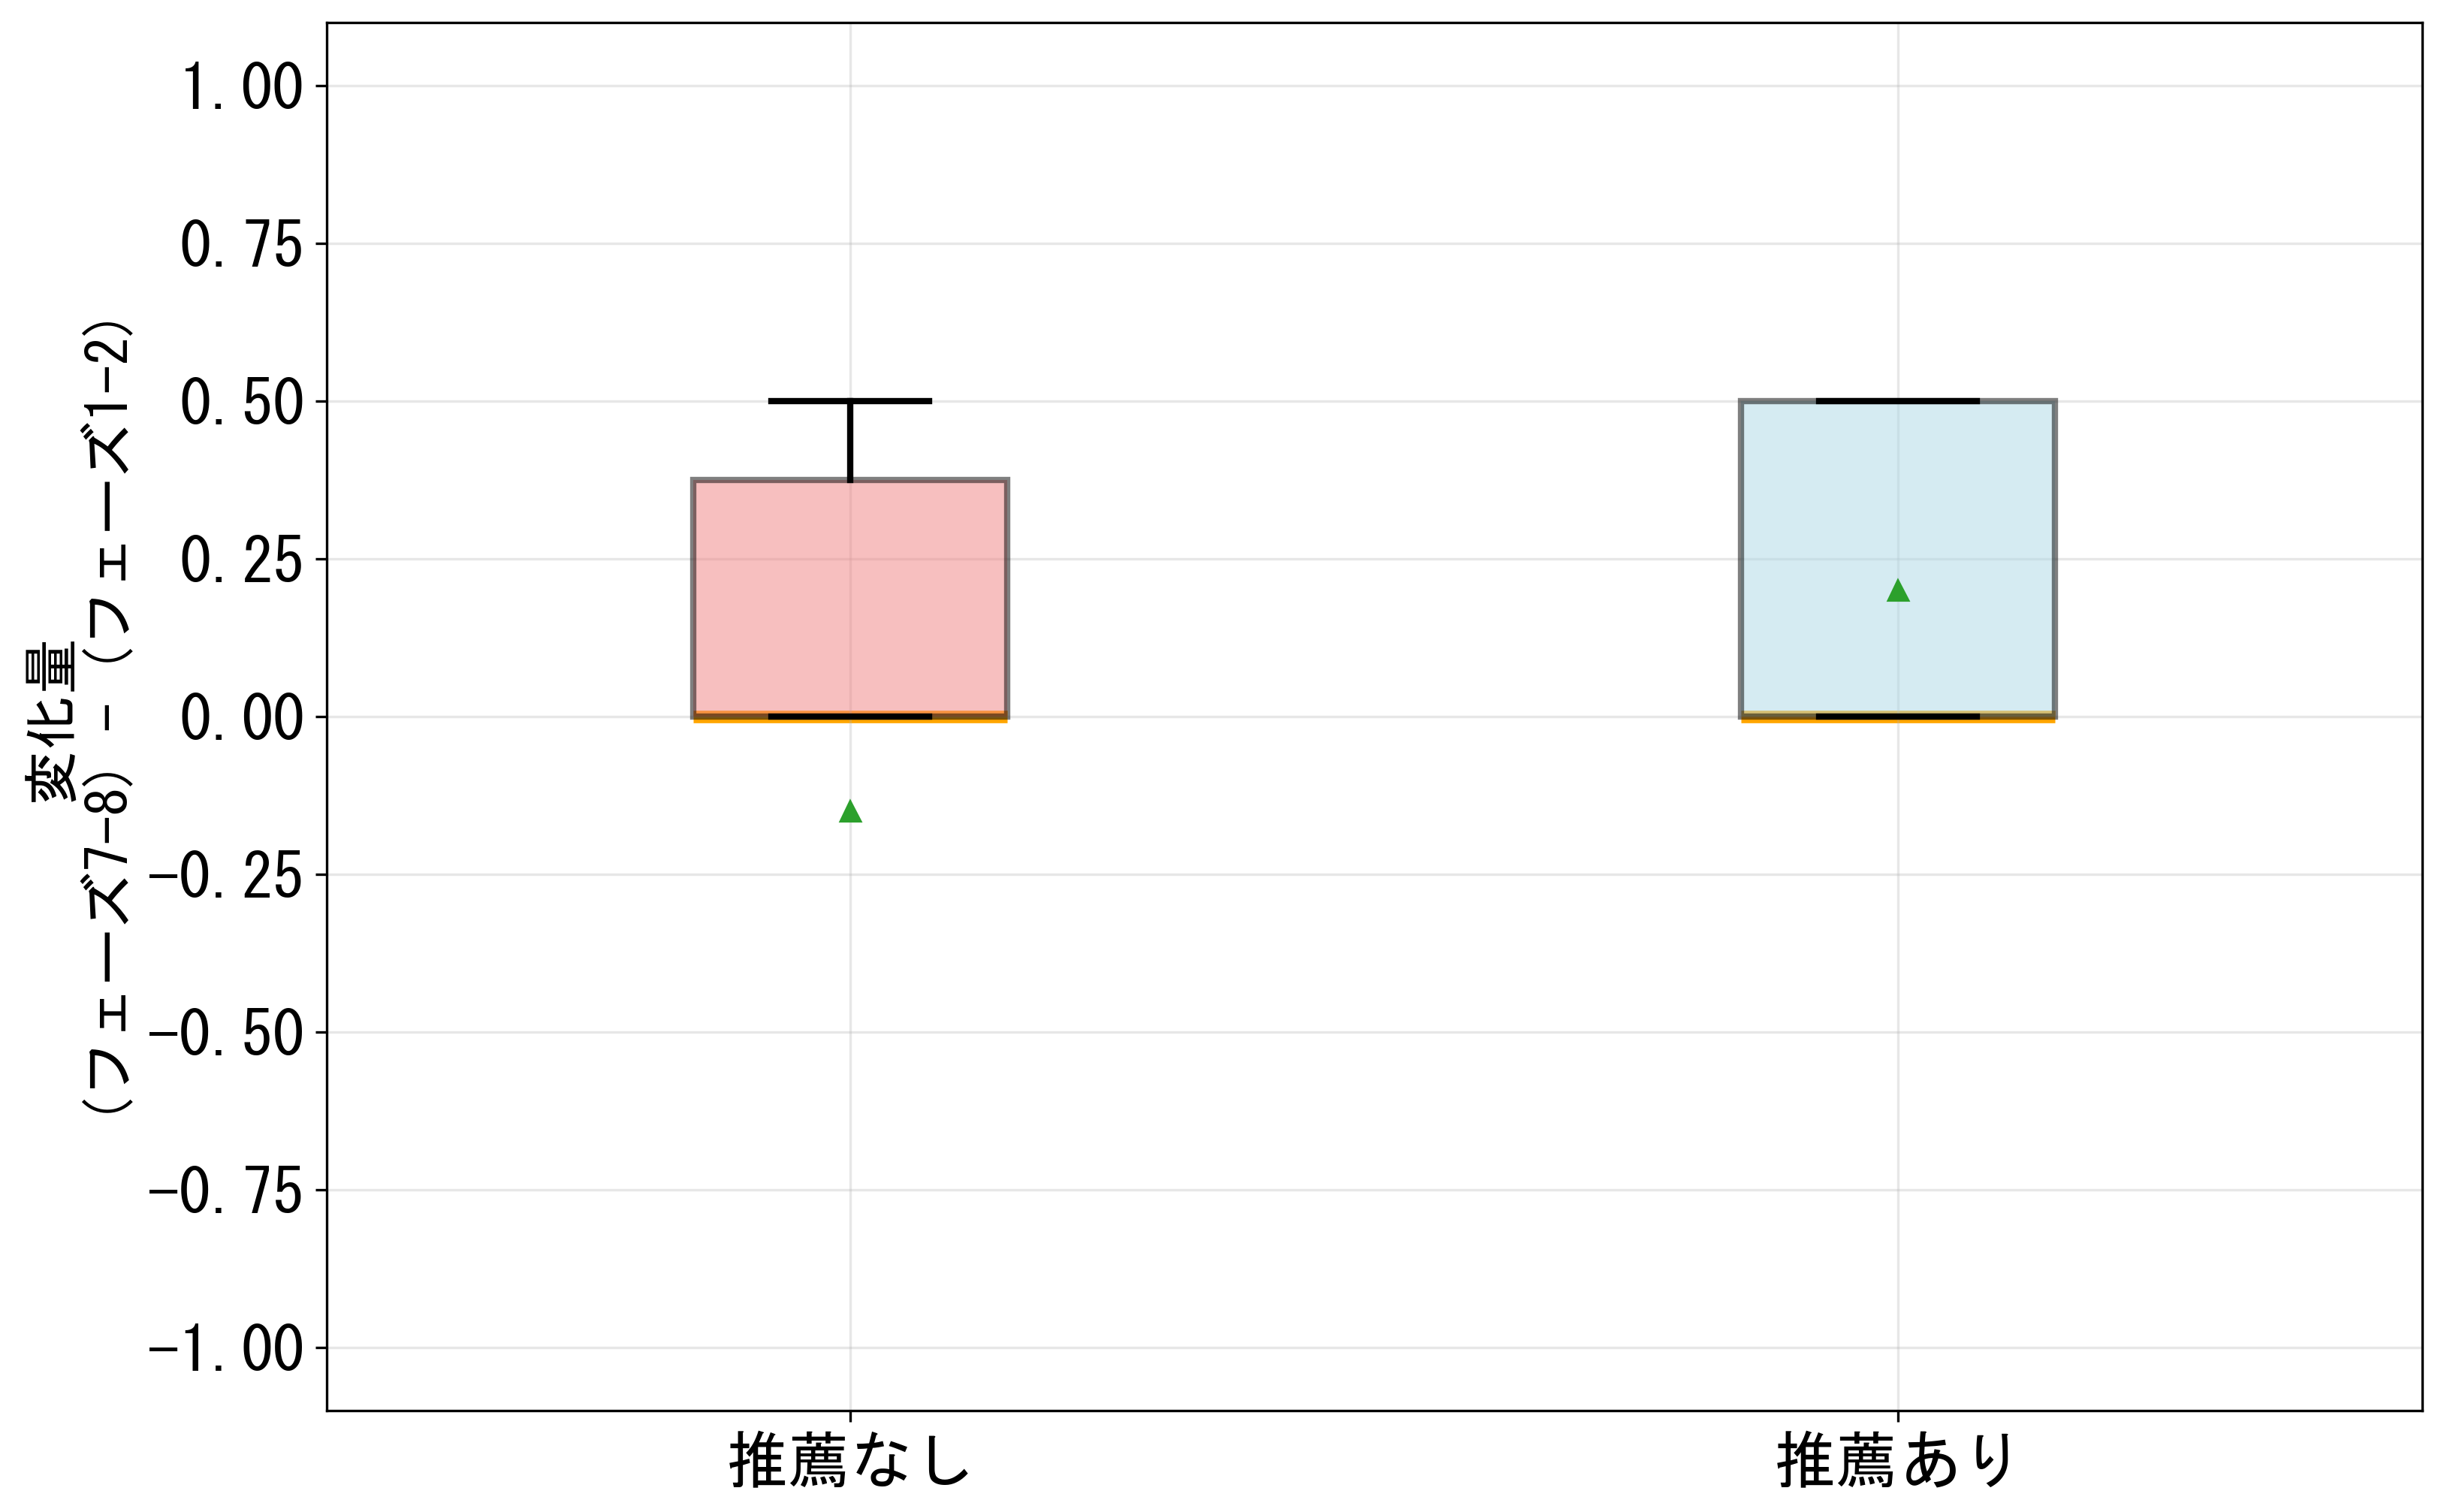
\includegraphics[width=0.9\linewidth]{image/EQ5_最終と序盤の差異_Box.png}
        \caption{EQ5: 序盤(フェーズ1-2)から終盤(フェーズ7-8)の変化量}
        \label{fig:EQ5-最初to最後の変化量}
    \end{figure}
    
    \begin{figure}[H]
        \centering
        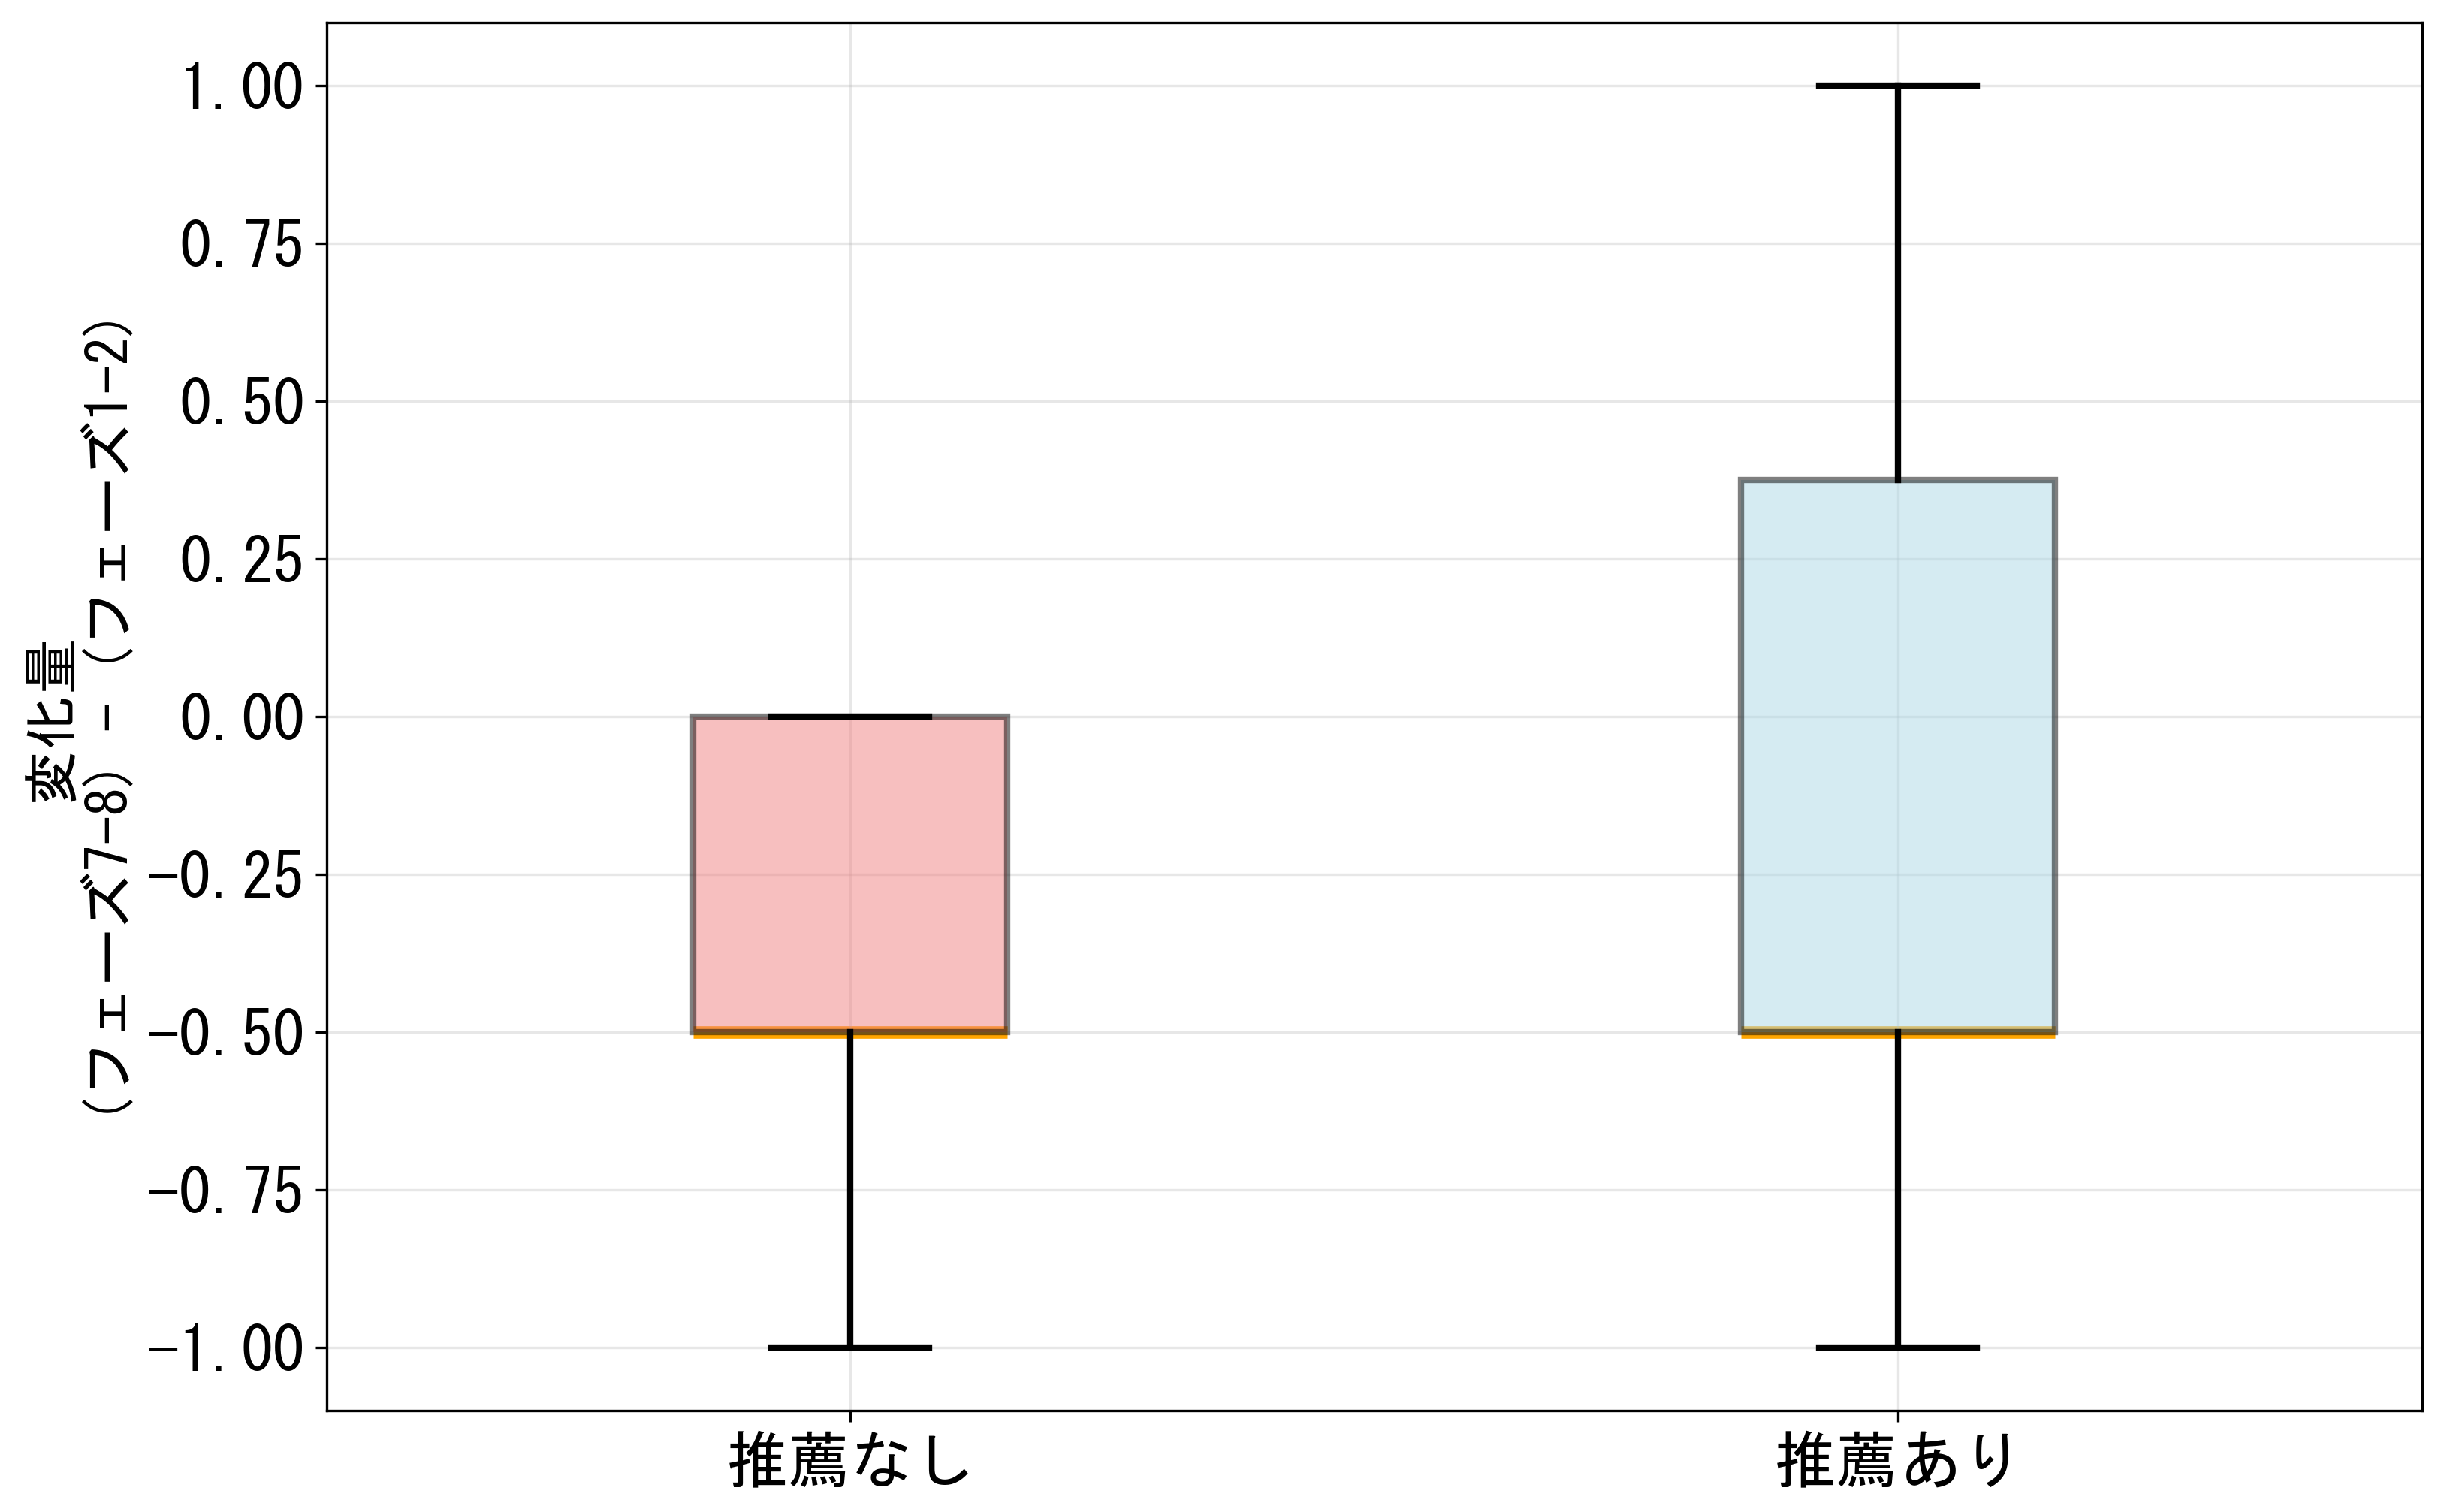
\includegraphics[width=0.9\linewidth]{image/EQ6_最終と序盤の差異_Box.png}
        \caption{EQ6: 序盤(フェーズ1-2)から終盤(フェーズ7-8)の変化量}
        \label{fig:EQ6-最初to最後の変化量}
    \end{figure}
\end{comment}

\section{考察}

本節では，主にヒアリングから得られた結果より，音楽嗜好を通じた自己開示の効果や，自己開示レベルの設定，推薦システムについて考察を行う．

\subsection{自己開示に関する考察}

本項では，音楽嗜好の共有が自己開示に与える影響について自己開示レベルの推移や，被験者の意見から考察を行う．

\subsubsection{自然な自己開示の傾向}
実験結果から，自由に選曲を行ったとき（推薦なし群）の自己開示の特徴的な傾向が明らかになった．表\ref{群別の自己開示レベルごとの曲数と人数}より，レベル4の自己開示が限定的であった一方で，レベル3の自己開示が頻繁に観察され，OとM以外の被験者全員がEQ5（聴いた曲について楽しく話ができた），EQ6（思いや経験が理解できた）で高スコア（4または5）を示した．この結果は，自己開示レベル3の曲が受容者にとって受け入れやすい曲であり，効果的な会話のきっかけとなったことを示唆している．

実験設計において曲に関する思い入れや経験の共有を主目的としたことで，自然と深い自己開示が促進されたと考えられる．レベル4の出現頻度が低かった主な要因として，曲の分類時に自己開示レベルの基準が不適切であった可能性が挙げられる．事後のヒアリングでは，ほとんどの被験者が強い思い入れのある曲を持っていたと報告しており，高いレベルの自己開示に該当するような曲があったにも関わらず，レベルの分類が不適切であった可能性がある．特に，「思い入れ」と「自己開示レベル」の関係性について，より精緻な基準設定が必要である．


\subsubsection{音楽嗜好の共有による自己開示}
楽曲に紐づいた個人的な経験や思い出が，自然な形で自己開示を促進することが確認された．例えば，高校時代の思い出や人生における重要な出来事，さらには恋愛体験などの個人的な経験が，楽曲を介して自然に共有されていた．これは音楽が「思い出の媒体」として機能し，通常の会話では語られにくい個人的な経験を引き出す触媒となることを示唆している．

音楽嗜好が自己開示を促す理由の1つに，長期的な友人関係においても，音楽を通じた新たな相互理解が促進されることが確認された．高校時代からの友人で頻繁にフェスに参加する被験者I,Jのペアでさえ，「こんな音楽も聴くんだってことを知れた」「自分の好きなものをたくさん伝えることができてよかった」と報告している．このことは，既知の関係性においても，音楽体験の共有が新たな一面の発見につながることを示唆している．
これらの結果から，音楽嗜好の共有は深い自己開示を促進する効果的な手段であることが実証された．音楽という媒体を介することで，より自然な形での自己開示が可能になると考えられる．


\begin{comment}
\subsubsection{楽曲への思い入れの影響}
楽曲に対する思い入れの強さが，自己開示の促進に強く結びついていることが明らかになった．思い入れの強い楽曲について語る際，より具体的かつ詳細な自己開示を行う傾向があることが分かった．
% 例えば，思い入れの強い楽曲では「年末のライブでこの曲を聴いた時の体験」や「この曲のここの歌い方が好きで」といった具体的な文脈を伴った自己開示が行われた．対照的に，思い入れの弱い楽曲では「知っている/知らない」や「他にどんな曲を出しているの？」といった表層的な会話に留まる傾向が見られた．
この結果は，楽曲への思い入れが強いほど，その曲に紐づいた個人的な体験や感情が豊富に存在し，それらの経験や感情が自然な会話の流れの中で語られやすくなることを示唆している．

音楽への関心度による影響も特徴的であった．音楽に対して深い関心を持つペアでは，楽曲の技術的な側面から個人的な体験まで，幅広く会話が展開された．一方で，音楽への関与度が比較的低いペアであっても，思い出という観点から会話が展開され，自己開示が自然に促進されることが確認された．
\end{comment}


\subsection{セッションについての考察}

本項では，音楽共有セッション自体の有効性について，被験者の意見や実験後のアンケートから分析を行う．特に，従来のカラオケとは異なる音楽共有セッションがもたらした効果について考察する．

\subsubsection{音楽を通じた会話をする楽しさ}
音楽共有セッションに対する被験者の反応は肯定的であった．19名の被験者が「楽しかった」と回答し，そのうち12名は「時間を忘れるほど楽しかった」「またこのセッションに参加したい」というように，音楽について相手と語り合う場に満足感を抱いていた．
実験後アンケートのPQ7（今後も相手と音楽の会話をしたい）も平均4.5と高スコアを記録し，曲を交互に聴き合い対話するというコミュニケーション形式が，相手との関係性を深める効果的な手段であることが示唆された．

% 「楽しかった」と答えた被験者は，音楽に対する思い入れや熱意がある人が多かった．曲に対しての自分のストーリーや物語がある人，聴いていた時の情景や時期を鮮明に覚えている場合などである．他にも，アーティスト自体への思い入れが強く，歌い方や音使いへのこだわりを話している人もいた．
一方で，「楽しめなかった」や「うまく話せなかった」と答えた被験者は，音楽への思い入れや過去の結びつきが少ないあるいは全くない人や，音楽について話す経験が不足している人であった．単純に曲が好きといった表面的な好みしか持たない人にとっては，深く話す内容がなく，会話を発展させることが難しかったという原因が考えられる．


\subsubsection{選曲時の意識}
選曲時の意識に関する実験結果から，重要な示唆が得られた．20人の被験者のうち14人は，選曲の基準として「思い入れや経験がある曲」「ストーリーとして話せそうな曲」など，個人的なエピソードと結びついた曲を重視していた．これは歌唱へのプレッシャーがない環境下で，より個人的な体験と結びついた曲を選びやすかったためと考えられる．
また，半数の被験者が「相手が知っていそうか」「好きそうな曲のジャンルか」という相手への配慮を示した．これは実際に相手に対して音楽を流すという形式が意識されていたことを示唆している．一方で，歌いやすさや普段のカラオケで歌う曲を意識した被験者は4人に留まった．

この結果は，本実験の設計に関する課題を明らかにしている．歌唱を伴わない音楽共有という形式は，通常のカラオケとは異なる選曲基準であった．実際のカラオケ環境では，曲を実際に歌う必要があり，歌唱力が試されるため自己開示の深さに影響を与える重要な要素となり得る．被験者からも「実際に歌わないから気楽に流すことができた」という意見が得られ，歌唱に対する心理的負担の有無が選曲基準に大きく影響することが確認された．

このことから，曲の自己開示レベルを構成する要素として設定した「歌いやすさ」は，本実験環境においては適切な指標ではなかった可能性が高い．今後は，歌唱を伴う実験との比較検証による選曲基準の違いの定量的分析が必要である．



\subsection{推薦システムについての考察}

本項では，推薦システムの提示方法や，段階的なアルゴリズムについての考察を行う．

\subsubsection{流れに合わせた選曲}
被験者からは「前の曲との流れを意識して選曲していた」「相手と同じアーティストの曲を入れた」といった意見があり，アーティストや楽曲間の関連性や，現在の雰囲気を考慮した推薦が自然な会話の展開を支援する可能性が示された．そのため，推薦システムの設計において，会話の流れと被験者の思い入れに応じた柔軟な選曲を支援することの重要性が明らかになった．
特に，推薦曲を強制的に選択させるのではなく，複数の選択肢から選べる提示方式の有効性が確認された．

ヒアリングの結果，最終フェーズでは「来て欲しい曲がこなかった」「今の雰囲気に合わなかった」という意見が得られた．これは，それまでの選曲の流れとは別に，個人的に共有したい楽曲が存在することを示している．
これらの知見から，自己開示を促進する音楽推薦システムには，現在の空気（会話の文脈や相手の選曲）に沿った推薦と個人の意図を反映できる柔軟性の両立が求められることが明らかになった．


\subsubsection{受容性を高める段階的なアプローチ}
HQ3（フェーズが進むにつれての楽曲選択意識の変化）への回答より，多くの被験者が前半で相手の知っている曲を意識的に選択していた．初期段階における共通点の活用が，音楽共有の受容性向上に効果的であることが明らかになった．これは，共通の楽曲が初期の会話の起点となり，「アニメ/ドラマの主題歌」といった共通の話題から会話を発展させやすいためと考えられる．
注目すべきは，4名の被験者から「共通の思い出のある曲から話が特に盛り上がった」という報告があった点である．「相手と初めて映画を見に行ったときの主題歌」（被験者S, T）や「2人でフェスに行ったときに感動した曲」（被験者I, J）といった，2人の思い出と結びついた楽曲が，受容性を大きく向上させることが示唆された．

これらの知見は，自己開示を促進する音楽共有において，共通知識や共有体験を基盤とした段階的なアプローチの有効性を示している．システム設計においては，初期段階で2人にとって関連のある楽曲を優先的に推薦することで，より自然な会話の展開が期待できる．
\begin{comment}

\section{グループごとに見る自己開示の有効性}
音楽嗜好を通じた自己開示の効果は，以下のような特徴的なグループ間で異なる傾向が観察された．効果が高い～低いまで，3つに分けて詳細を述べる．


\subsubsection{高効果グループ（6ペア，12名）}
% [メモ：I-J, Q-R, S-T, G-H, C-D, K-L]
音楽活動への積極的な参加や日常的な音楽体験を持つグループでは，音楽嗜好の共有を通じた自己開示が特に効果的であった．このグループの被験者は，楽曲に対する具体的な思い入れや経験を豊富に持ち，音楽を通じた対話に対して積極的な態度を示した．特筆すべき点として，楽曲についての技術的な議論から個人的な体験の共有まで，多層的な対話が自然に展開される傾向が見られた．また，相手の知らない楽曲であっても，その楽曲にまつわる個人的な体験や解釈を積極的に共有する様子が観察された．


\subsubsection{中程度効果グループ（3ペア，6名）}
% [メモ：A-B, O-P, L-M]
一般的な音楽愛好者層に相当するグループでは，共通の経験や思い出を持つ楽曲を中心に対話が展開された．このグループの特徴として，段階的に自己開示の深さを増していく傾向が観察された．特に，相手の反応を確認しながら慎重に対話を進める様子が見られ，共通の文脈を持つ楽曲（アニメやドラマの主題歌など）を通じて自己開示が促進される傾向が確認された．

\subsubsection{効果が限定的なグループ（1ペア，2名）}
% [メモ：E-F]
音楽への関与度に大きな差があるペアでは，音楽嗜好の共有を通じた自己開示に困難が見られた．このグループでは，音楽を通じた対話に不安や困難を感じる様子が観察され，楽曲に対する思い入れや経験の共有が限定的となる傾向が確認された．特に，音楽について話すことへの心理的障壁が，自然な対話の展開を妨げる要因となっていた．

\vskip\baselineskip
これらのグループ間での主な差異として，対話の深さ，楽曲選択の特徴，自己開示の質において顕著な違いが観察された．高効果グループでは多層的で深い対話が自然に展開されたのに対し，中程度グループでは段階的な深化が特徴的であり，効果が限定的なグループでは表層的な対話に留まる傾向が見られた．

\end{comment}

% 5章
\chapter{結論}

本章では，本研究のまとめと今後の課題について述べる．

\section{まとめ}

本研究では，音楽嗜好の共有を通じた段階的な自己開示が受容性に与える影響について検討した．若者の深い自己開示を避ける傾向に対し，音楽嗜好の共有を通じた自己開示を提案し，カラオケ環境を想定した音楽共有セッションにおいて，段階的な自己開示を促す楽曲推薦システムを開発し，その効果を実証的に検証した．

実験からは，低レベルから高レベルの自己開示へと段階的に行うことで，高いレベルの自己開示に対する受容度が維持されることが確認された．システムによる段階的な推薦を受けた群は，後半フェーズで高いレベルの自己開示を促されているにも関わらず，推薦なし群と同等の高い受容度を維持していた．また，相手の音楽への認知度や興味度が低い場合でも，自己開示の受容度は大きく低下しないことが示された．これは，音楽を通じたコミュニケーションが，楽曲そのものへの興味の有無に関わらず，相手の経験や感情を受容できることを示唆している．さらに，音楽嗜好の共有は単なる趣味の共有を超えて，個人的な経験や価値観の自然な開示を促進することが明らかになった．

ヒアリングの結果からは，音楽をきっかけとしたコミュニケーションが長期的な友人関係においても新たな相互理解を促進されることが分かった．これらの知見は，音楽嗜好の共有が自己開示を促進し，人間関係の親密化に寄与する効果的な手段となり得ることを実証的に示している．


\section{今後の課題}

本研究には，いくつかの課題が残されている．歌唱を伴う実際のカラオケ環境での検証は重要な課題である．本実験では歌唱を除外した環境で基礎的な知見を得たが，実際のカラオケでは歌唱技術やプレッシャーが自己開示の深さに影響を与える可能性がある．今後は歌唱を含めた実験を行い，より実践的な知見を得る必要がある．

自己開示レベルの分類基準の精緻化も求められる．実験結果から，特に「思い入れ」と「自己開示レベル」の関係性について，より詳細な基準設定が必要であることが明らかになった．楽曲に対する個人的な意味づけをより適切に評価できる指標の検討も求められる．

また，本研究では20名という限られたサンプルサイズでの検証に留まっている．特に推薦システムの効果検証において，統計的な有意差を得るためには，より大規模なデータでの分析が必要である．様々な年齢層や関係性を持つペアでの検証を通じて，本手法の一般性を確認することも重要な課題である．

今後は，これらの課題に取り組むことで，音楽嗜好の共有を通じた自己開示の促進と受容に関する理解がさらに深まることが期待される．
% 6章
% \input{./6th/chapter6}


% 謝辞
\chapter*{謝辞}
岩本先生，高田くん，実験協力してくれた20名の被験者，論文を添削してくれた山北さん，高田くん，二村くん，本当にありがとう！
OBの鈴木さん，山内さん，藤尾さんにもスーパー感謝です！！

% 本研究を進めるにあたり，研究の内容，論文の執筆など，終始適切なご指導を賜りました，岩本健嗣教授には心から感謝申し上げます．
% 実験協力してくれた20名の被験者に感謝
% 論文の添削してくれた先輩方
% 高田のこともかく
% ここに謹んでお礼申し上げます．

\addcontentsline{toc}{chapter}{\numberline{}謝辞}

% 参考文献
\newpage
\addcontentsline{toc}{chapter}{\numberline{}参考文献}
\bibliography{cite}
\bibliographystyle{ipsjunsrt}

\end{document}